\appendix

\chapter{Comparaciones por Género}\label{ApendiceA}

En este apéndice se presentan más resultados de los modelos discutidos en esta tesis, que no se abordaron con detalle en el Capítulo 4. Aquí se encontrarán los análisis exploratorios del modelo ajustado para hombres y del modelo ajustado para mujeres, junto con sus respectivas interpretaciones. Además, se incluyen las comparaciones finales entre ambos modelos. Esta información adicional proporciona una comprensión más profunda de las diferencias y similitudes en las relaciones entre variables según el género, permitiendo una evaluación más completa y matizada de los resultados.

%%%%%%%%%%%%%%%%%%%%%%%%%%%%%%%%%%%%%%%%%%%%%%%%%%%%%%
%%%%%%% A N A L I S I S  P O R  G E N E R O %%%%%%%%%%
%%%%%%%%%%%%%%%%%%%%%%%%%%%%%%%%%%%%%%%%%%%%%%%%%%%%%%

\section{Boxplot Funcionales por Género}

Antes de comenzar el análisis de los modelos ajustados, se realizaron boxplots funcionales para comparar las diferencias en el comportamiento de las curvas de glucosa e insulina por género en cada prediagnóstico. Este análisis preliminar tiene como objetivo comprender mejor la naturaleza del procesamiento de glucosa en los diferentes géneros, proporcionando una base sólida para interpretar los modelos ajustados posteriormente.

En la Figura \ref{fig:glucosaNormal}, se muestra una comparación de los boxplots funcionales entre hombres y mujeres de individuos cuyo prediagnóstico es normal. En la curva mediana de ambos boxplots, se observa una tendencia creciente seguida de un descenso. Sin embargo, en la curva mediana asociada a hombres, el pico se alcanza a los $30$ minutos y luego desciende, mientras que en las mujeres, el pico parece estar entre los $30$ y $60$ minutos antes de descender. Este comportamiento también se observa en la curva del tercer cuartil. Este comportamiento coincide con hallazgos de estudios previos que comparan la homeostasis entre hombres y mujeres, donde se concluye que las mujeres suelen mostrar niveles más bajos de glucosa al inicio de la prueba oral de tolerancia a la glucosa y terminan con niveles más altos \cite{GenderDifferences2018}.

Adicionalmente, en las curvas asociadas al primer cuartil en ambos casos, se observa un descenso seguido de un ascenso, lo que sugiere posibles errores de medición.


\begin{figure}[H]
 \centering
  \subfloat[Mujeres]{
   \label{bfMuGluNormal}
    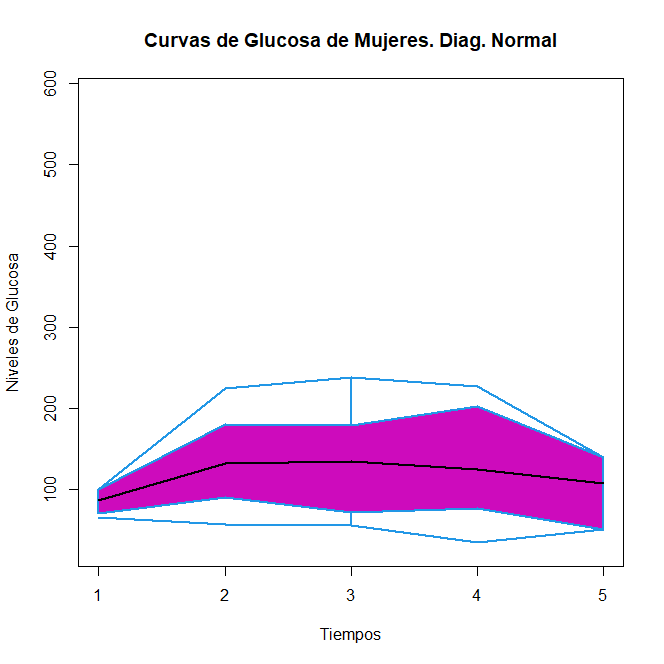
\includegraphics[width=0.45\textwidth]{img/bfMujgluNormal.png}}
  \subfloat[Hombres]{
   \label{bfHoGluNormal}
    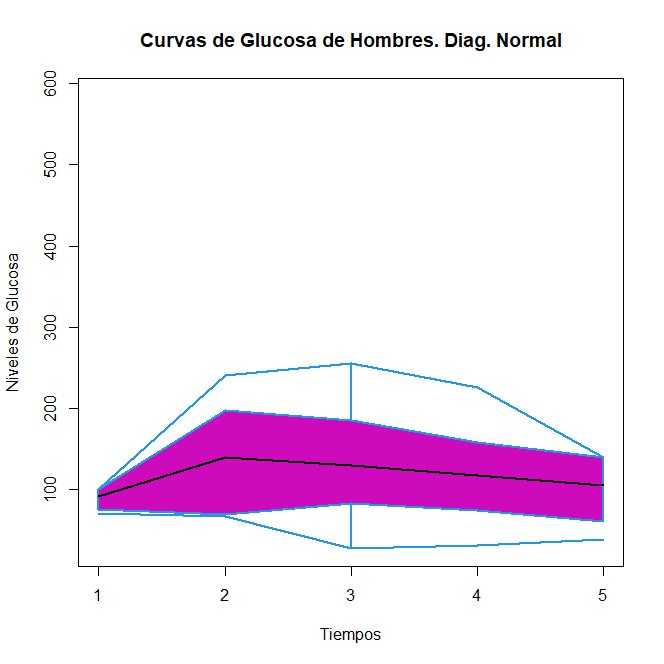
\includegraphics[width=0.45\textwidth]{img/bfHogluNormal.png}}
    \caption{Boxplot funcional para las curvas de glucosa para personas con prediagnóstico normal.}
    \label{fig:glucosaNormal}
\end{figure}

Los boxplots correspondientes a las curvas de insulina de la Figura \ref{fig:insulinaNormal}, muestran un comportamiento similar en ambos géneros, con una curva mediana ascendente seguida de un descenso, aunque en el caso de los hombres esta curva parece ser más pronunciada.

Es importante destacar que en el boxplot correspondiente a mujeres se observan varios outliers, con niveles de insulina bastante altos. Esto sugiere la posibilidad de que estos individuos estén experimentando resistencia a la insulina, aunque esta condición aún no se refleje claramente en su curva de glucosa. Por otro lado, la curva del primer cuartil muestra niveles bajos en ambos casos.

En cuanto al tercer cuartil, la curva de las mujeres se asemeja bastante a la curva correspondiente a la mediana, lo que sugiere una forma común. Sin embargo, en los hombres esta curva se modifica ligeramente posiblemente algún error de medición. 

De acuerdo con el articulo `\textit{Gender Differences in Glucose Homeostasis and Diabetes}' \cite{GenderDifferences2018} las mujeres, en comparación con los hombres de la misma edad, tienden a tener menor masa muscular esquelética y mayor masa de tejido adiposo, así como mayores niveles circulantes de ácidos grasos libres (FFA) y un contenido lipídico intramiocelular elevado. Estos factores podrían promover la resistencia a la insulina en las mujeres. A pesar de estas diferencias, las mujeres son tan sensibles a la insulina como los hombres.


\begin{figure}[H]
 \centering
  \subfloat[Mujeres]{
   \label{bfMuGluInsulina}
    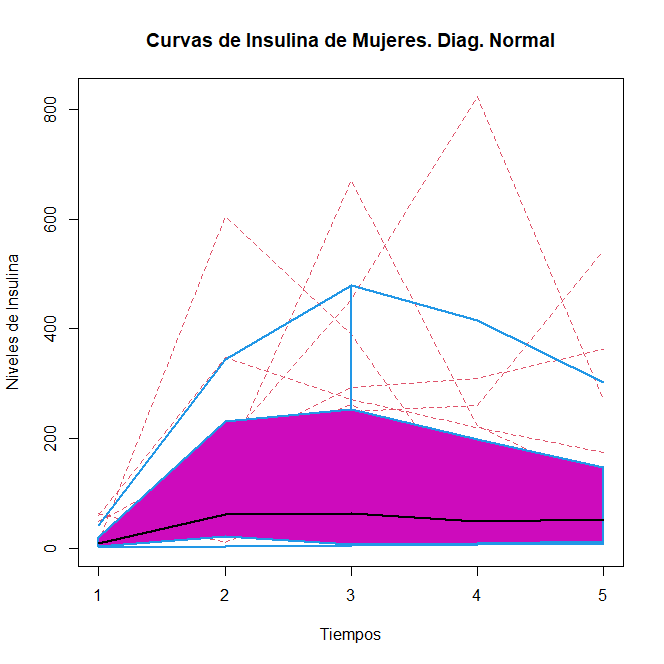
\includegraphics[width=0.45\textwidth]{img/bfMuInsNormal.png}}
  \subfloat[Hombres]{
   \label{bfHoGluInsulina}
    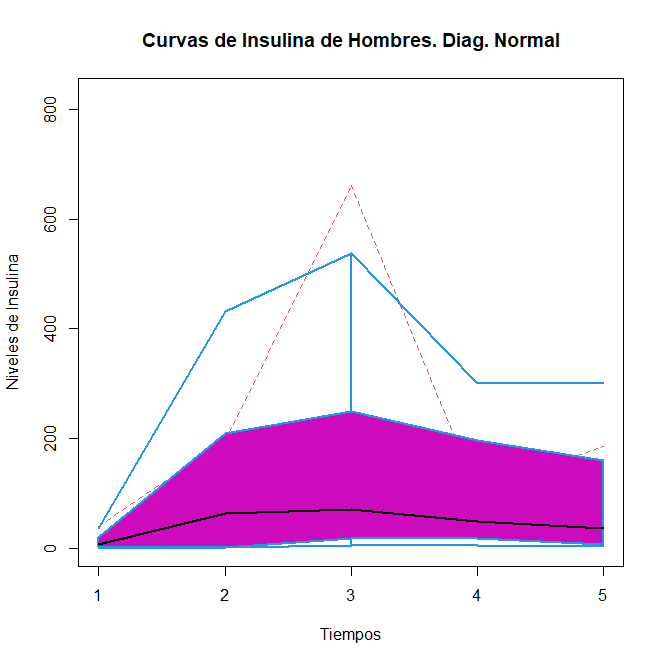
\includegraphics[width=0.45\textwidth]{img/bfHoInsNormal.png}}
    \caption{Boxplot funcional para las curvas de insulina para personas con prediagnóstico normal.}
    \label{fig:insulinaNormal}
\end{figure}


%%%%%%%%%%%%%%%%%%%%%%%%%%%%%%%%%%%%%%%%%%%%%%%%%%%%%%%%

En la categoría de prediabéticos, la Figura \ref{fig:glucosaPredia} indica que los boxplots funcionales de glucosa para hombres y mujeres muestran diferencias significativas. La curva mediana en mujeres es ascendente hasta el minuto $90$ y luego comienza a descender, mientras que en hombres alcanza su máximo a los $60$ minutos. El tercer cuartil presenta un comportamiento similar, aunque en mujeres parece haber una mayor resistencia a la insulina, ya que los valores de glucosa no disminuyen tanto.

La curva del primer cuartil correspondientes a hombres y mujeres muestra nuevamente un patrón ascendente, descendente y posteriormente ascendente, lo que podría sugerir otro posible error de medición. Por otro lado, la curva del bigote inferior de mujeres parece seguir la misma forma que la curva mediana de mujeres, lo que sugiere una tendencia común en este grupo.

Adicionalmente, a los $120$ minutos, los valores de las curvas de glucosa de las mujeres tienen una varianza mayor que la de los hombres. 

La prevalencia de síndromes pre-diabéticos, como la glucosa en ayuno alterada (IFG) y la tolerancia alterada a la glucosa (IGT) que corresonden a niveles de glucosa a las dos horas entre $140$ y $199$, también presenta un sesgo sexual \cite{GenderDifferences2018}. Específicamente, la IFG es más prevalente en los hombres, mientras que la IGT es más común en las mujeres. Estas diferencias destacan la importancia de considerar el sexo como un factor en el diagnóstico y tratamiento de condiciones pre-diabéticas, ya que hombres y mujeres pueden presentar distintos riesgos y necesidades en el manejo de su salud metabólica \cite{GenderDifferences2018}.

\begin{figure}[H]
 \centering
  \subfloat[Mujeres]{
   \label{bfMuGluPredia}
    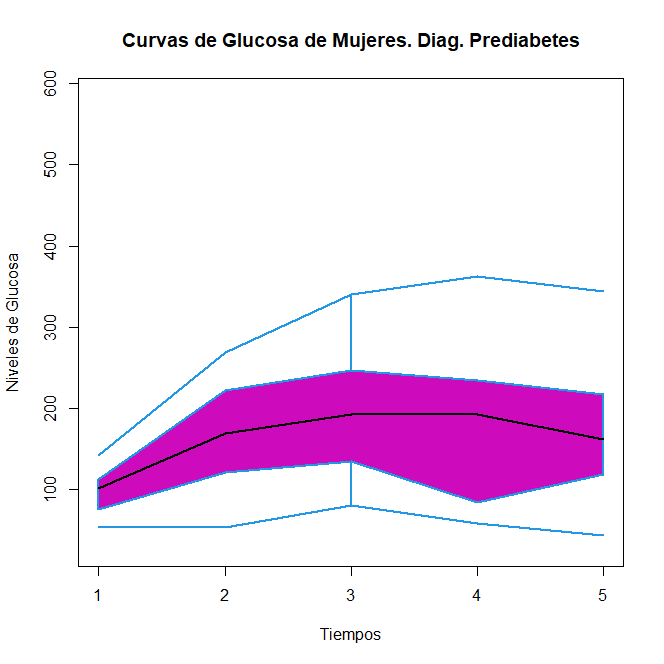
\includegraphics[width=0.45\textwidth]{img/bfMugluPredia.png}}
  \subfloat[Hombres]{
   \label{bfHoGluPredia}
    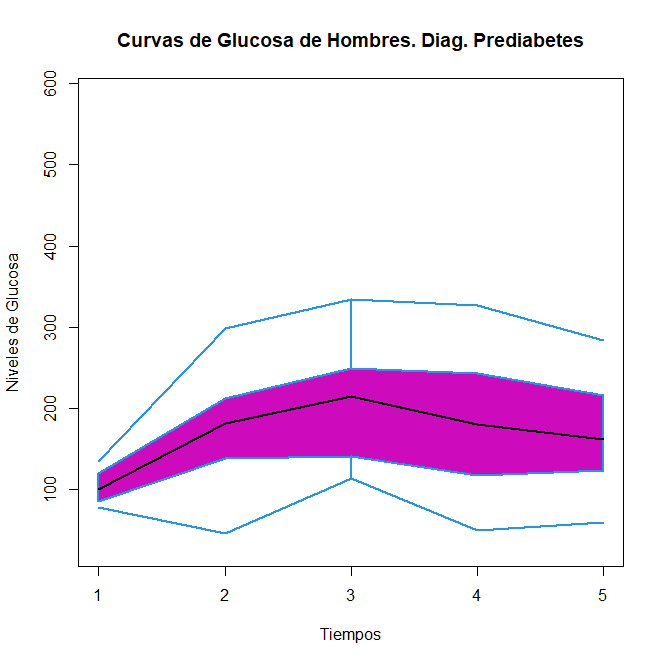
\includegraphics[width=0.45\textwidth]{img/bfHogluPredia.png}}
    \caption{Boxplot funcional para las curvas de glucosa para personas con prediagnóstico prediabetes.}
    \label{fig:glucosaPredia}
\end{figure}


En la Figura \ref{fig:insulinaPredia}, se muestran los boxplots funcionales de las curvas de insulina de ambos géneros en individuos prediabéticos. Uno de los aspectos más destacables son los outliers, que en ambos casos presentan valores muy altos. Este comportamiento podría ser indicativo de individuos con una resistencia a la insulina significativa, que están al borde de desarrollar diabetes.

\begin{figure}[H]
 \centering
  \subfloat[Mujeres]{
   \label{bfMuInsPredia}
    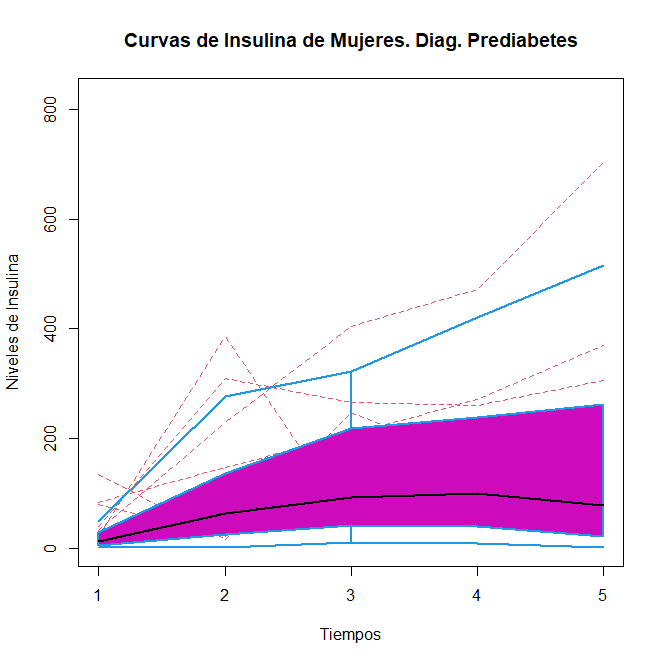
\includegraphics[width=0.45\textwidth]{img/bfMuInsPredia.png}}
  \subfloat[Hombres]{
   \label{bfHoInsPredia}
    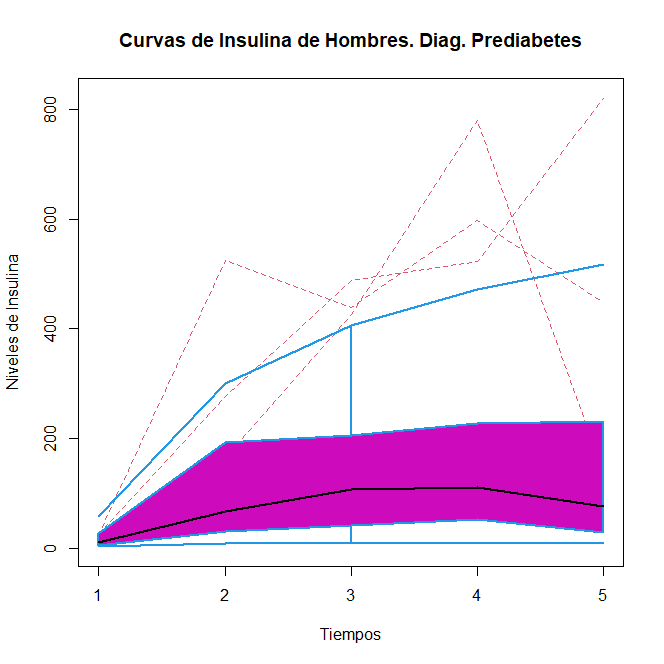
\includegraphics[width=0.45\textwidth]{img/bfHoInsPredia.png}}
    \caption{Boxplot funcional para las curvas de insulina para personas con prediagnóstico prediabetes.}
    \label{fig:insulinaPredia}
\end{figure}

En las mujeres, la curva mediana alcanza su máximo en el minuto $90$, y el tercer cuartil se encuentra más separado de la mediana en comparación con el primer cuartil, lo que evidencia valores altos en los datos. Además, se aprecia una mayor varianza en los valores del minuto 120 en las mujeres en comparación con los hombres.


En los hombres, la curva mediana parece ser similar a la de las mujeres, pero los valores del tercer cuartil son ligeramente más bajos. Estos boxplots pueden resultar difíciles de discernir en cuanto a esta categoría, ya que la curva del primer cuartil es muy baja tanto en hombres como en mujeres, lo que podría indicar individuos con diabetes, y también se observan curvas muy altas.


%%%%%%%%%%%%%%%%%%%%%%%%%%%%%%%%%%%%%%%%%%%%%%%%%%

En la categoría diabética la cual se presenta en la Figura \ref{fig:glucosaDiabetes}, en ambos boxplots funcionales las curvas medianas de glucosa se encuentran en un rango alto, alcanzando su máximo en el minuto $90$ para luego descender, ver Figura \ref{fig:glucosaDiabetes}. Sin embargo, en el caso de los hombres, la curva media desciende más rápidamente en comparación con las mujeres, donde parece ser más gradual. Es importante destacar que la varianza en el último instante es mayor en hombres, y se observa que el bigote superior alcanza niveles de alrededor de $600$.

\begin{figure}[H]
 \centering
  \subfloat[Mujeres]{
   \label{bfMuGluDia}
    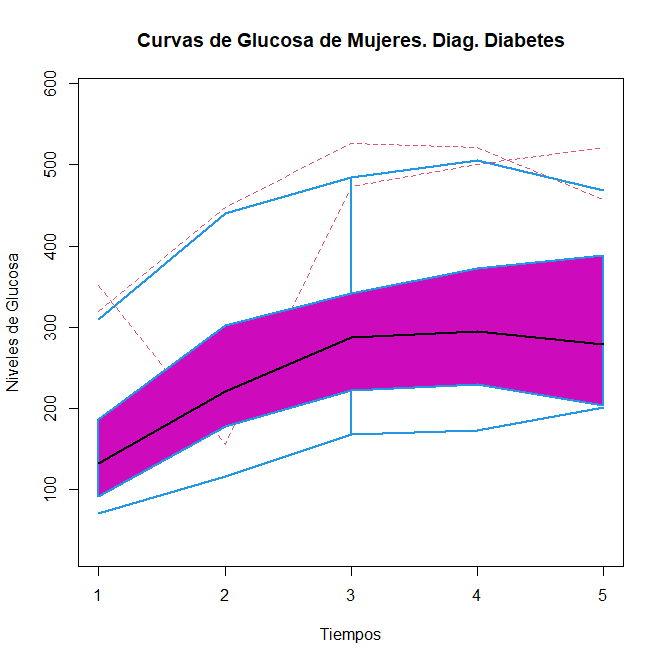
\includegraphics[width=0.45\textwidth]{img/bfMugluDiab.png}}
  \subfloat[Hombres]{
   \label{bfHoGluDia}
    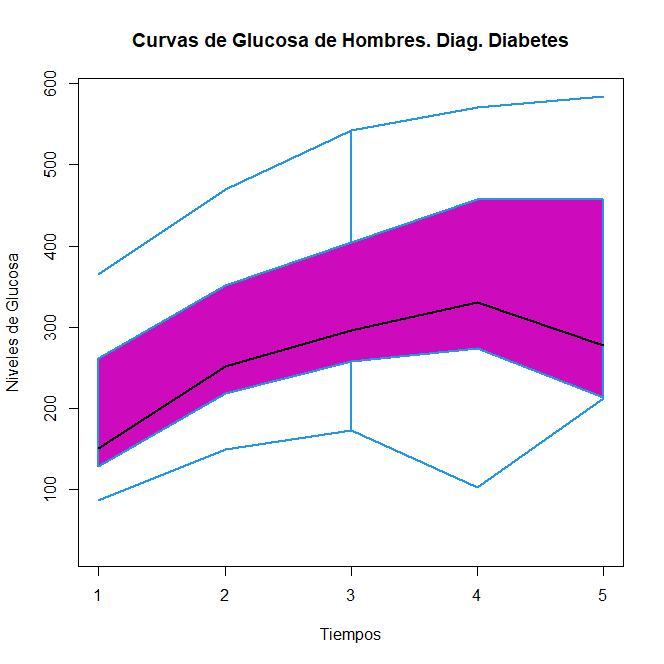
\includegraphics[width=0.45\textwidth]{img/bfHoGluDiabetes.png}}
    \caption{Boxplot funcional para las curvas de glucosa para personas con prediagnóstico diabetes.}
    \label{fig:glucosaDiabetes}
\end{figure}

Además, es notable que en esta categoría casi no hay outliers; en el boxplot de hombres no se presentan, y en el de mujeres hay dos, uno de los cuales muestra una caída muy abrupta en el minuto $30$, lo cual es biológicamente poco plausible y podría atribuirse a un error de medición. Similarmente, se observa una caída repentina en el bigote inferior de los hombres en el minuto $90$, lo que también podría ser atribuido a un error tipográfico.

En ambos casos parece haber un patrón discernible: en los hombres, el ascenso alcanza rangos más altos, mientras que en las mujeres parece ser un poco más suave. Sin embargo, sería difícil afirmar que esta diferencia es característica de cada género, ya que puede haber variabilidad individual significativa dentro de cada grupo.

La prevalencia de la diabetes tipo 2 también se caracteriza por una diferencia de sexo, de acuerdo a los resultados de los estudios realizados en \cite{GenderDifferences2018}. En general, la prevalencia global de diabetes es mayor en hombres, pero hay más mujeres con diabetes que hombres.

\begin{figure}[H]
 \centering
  \subfloat[Mujeres]{
   \label{bfMuInsDia}
    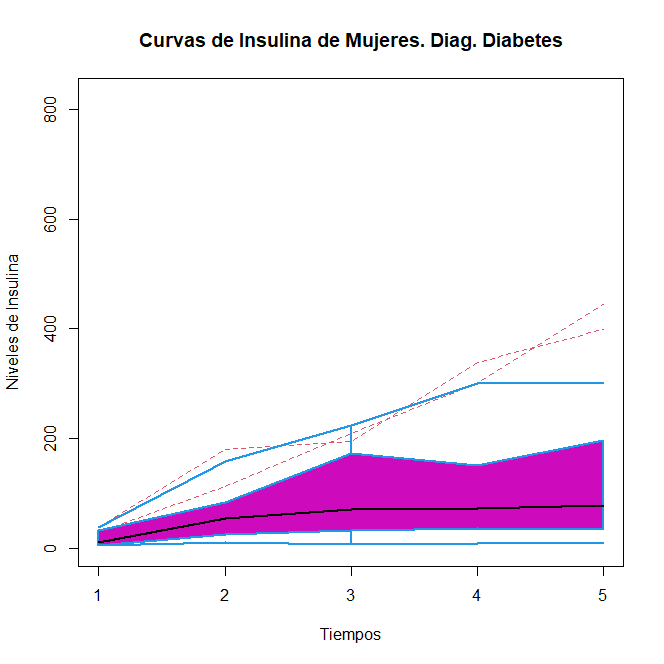
\includegraphics[width=0.45\textwidth]{img/bfMuInsDiabetes.png}}
  \subfloat[Hombres]{
   \label{bfHoInsDia}
    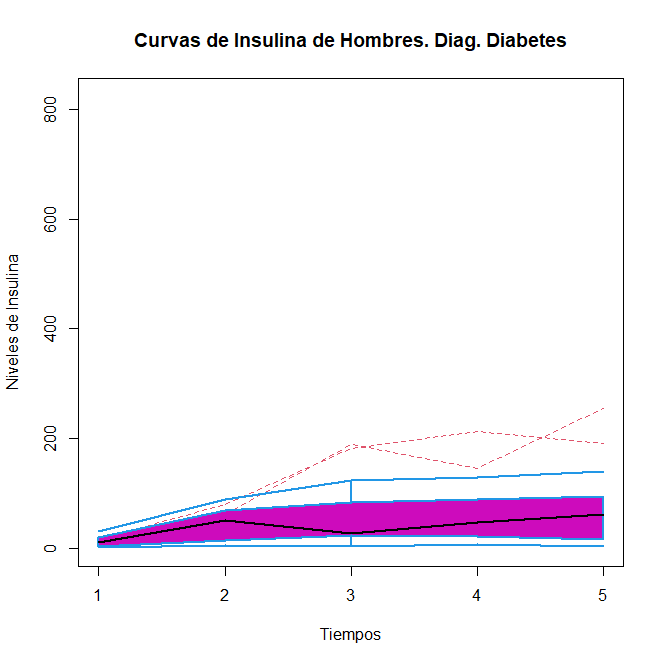
\includegraphics[width=0.45\textwidth]{img/bfHoInsDiabetes.png}}
    \caption{Boxplot funcional para las curvas de insulina para personas con prediagnóstico diabetes.}
    \label{fig:insulinaDiabetes}
\end{figure}

Los boxplots funcionales correspondientes a las curvas de insulina de la categoría diabética se muestran en la Figura \ref{fig:insulinaDiabetes}. Estos boxplots parecen presentar características significativas. La curva mediana correspondiente al grupo de hombres es más baja que la de mujeres. Por otro lado, las curvas asociadas al primer y tercer cuartil de la categoría de hombres están muy cercanas a la mediana, lo que indica poca variabilidad. En cambio, las curvas del primer y tercer cuartil de mujeres están más separadas, lo que indica mayor variabilidad.

Varias curvas representativas de ambos boxplots muestran el comportamiento inusual de subir, bajar y luego volver a subir. Aunque estos cambios pueden atribuirse a errores de medición, dado que no son extremadamente abruptos, no se descartarán. Los outliers son de escala, sin embargo, siguen este patrón de solo ascenso y en cantidades reducidas, lo cual concuerda con el perfil diabético.


%%%%%%%%%%%%%%%%%%%%%%%%%%%%%%%%%%%%%%%%%%%%%%%%%%%%%%%%%%%%%
%%%%%%%%%%%%%%%%%%%%%%%%%%%%%%%%%%%%%%%%%%%%%%%%%%%%%%%%%%%%%
%%%%%%%%%%%%%%%%%%%%%%%%%%%%%%%%%%%%%%%%%%%%%%%%%%%%%%%%%%%%%

\begin{landscape}
\subsection{Visualización del Modelo Ajustado para Mujeres}

\begin{figure}[H]
    \centering
    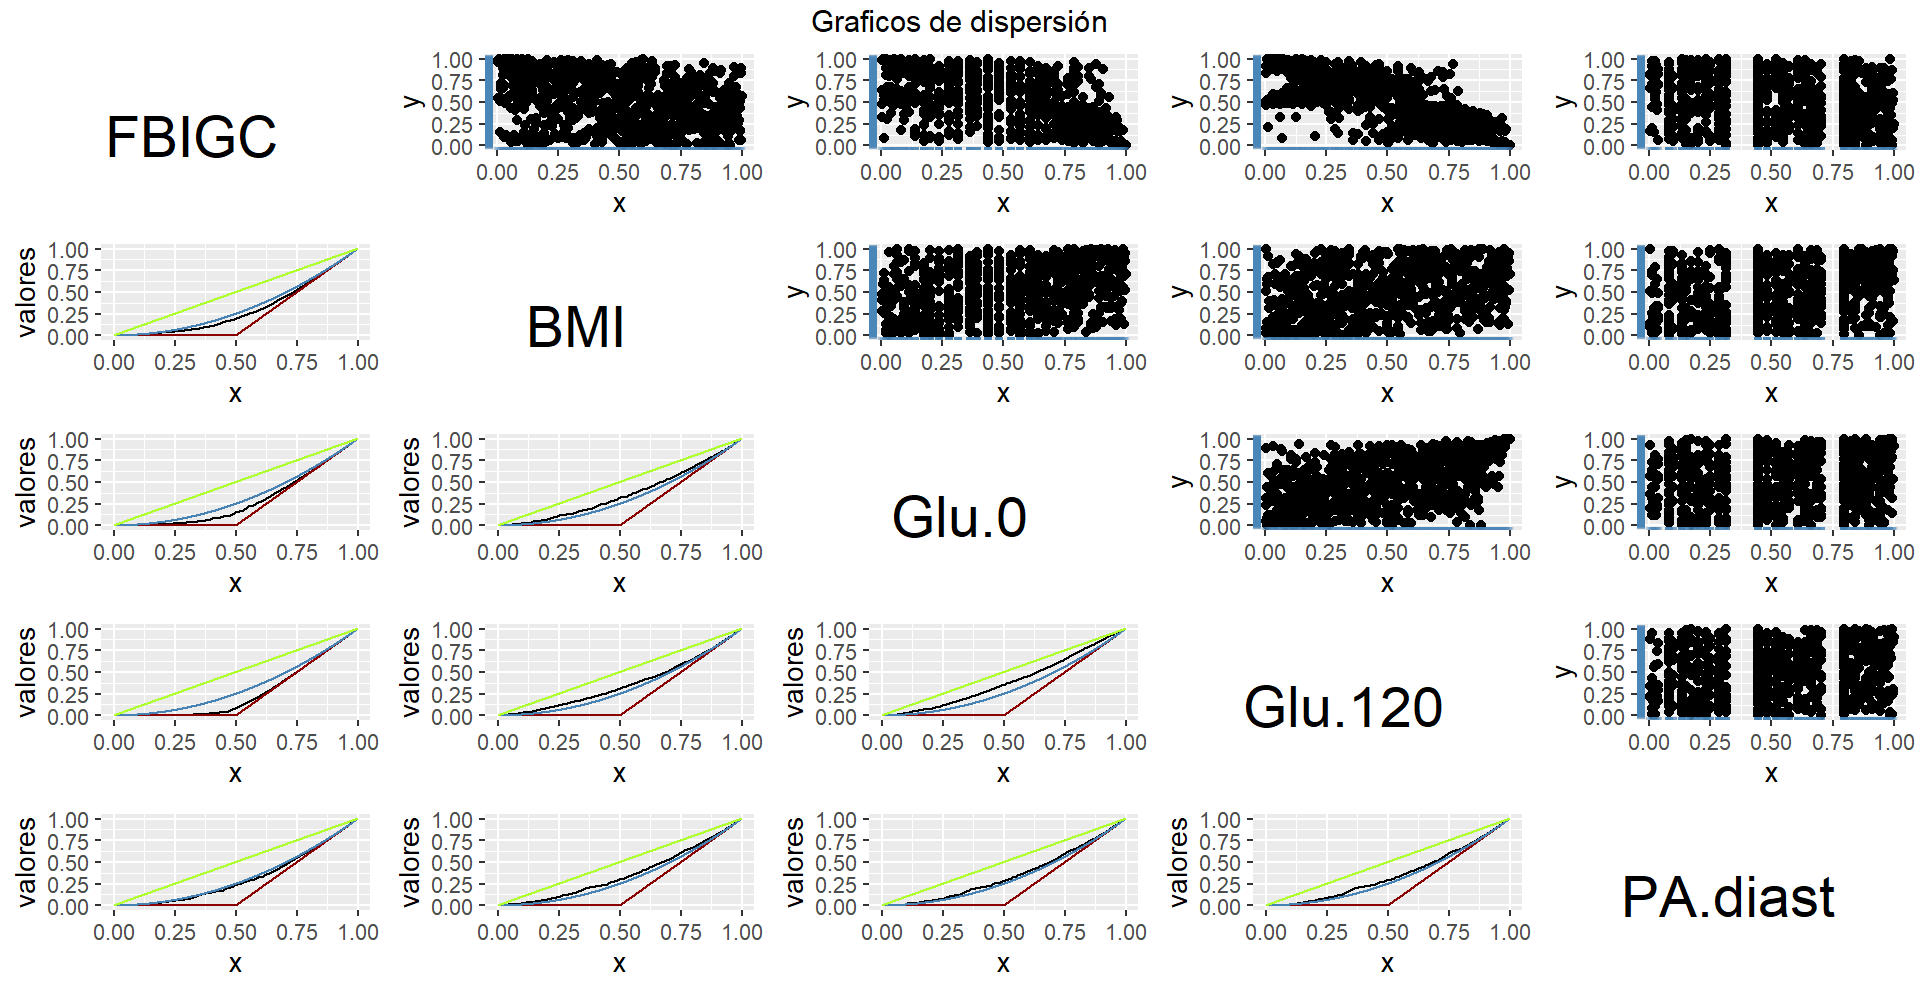
\includegraphics[height = 13.5 cm, width = 1.4 \textwidth]{4img/UdiagM.png}
    \caption{Diagonales y gráficos de dispersión en escala $u$ de mujeres.}
    \label{fig:diagMU}
\end{figure}
\end{landscape}

En la Figura \ref{fig:diagMU}, se presentan las diagonales de las cópulas empíricas con respecto a las diagonales de cópulas de referencia, junto con los gráficos de dispersión de las variables de individuos del género femenino. Al igual que en el caso de hombres y mujeres, expuesto en el Capítulo \ref{Resultados}, Figura \ref{fig:diagTot}. En su mayor parte, la diagonal de la cópula empírica se encuentra por debajo o por encima de la diagonal, lo que indica que las dependencias entre las variables son mayoritariamente concordantes negativas o positivas, respectivamente. También se observa la misma partición generada por la variable de presión diastólica.


\begin{figure}[H]
 \centering
  \subfloat[$\mathscr{H}\rho_{C_{12}}$]{
   \label{C12rho}
    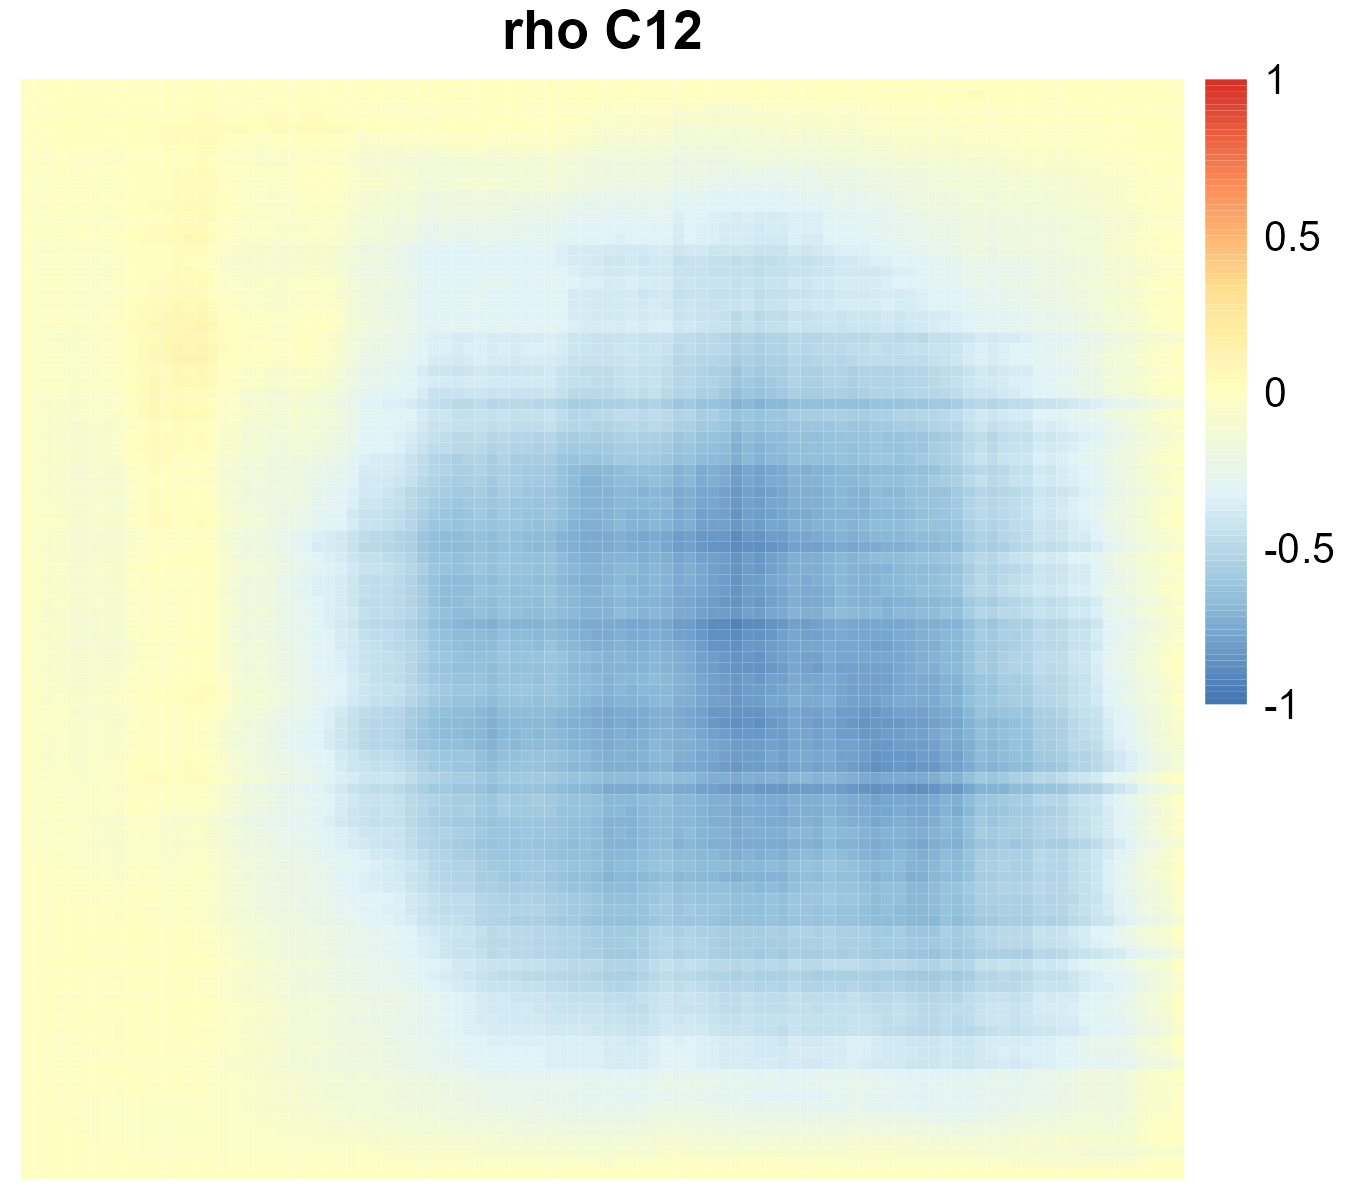
\includegraphics[width=0.33\textwidth]{4img/MujrhoC12.png}}
  \subfloat[$\mathscr{H}\sigma_{C_{12}}$]{
   \label{C12sigma}
    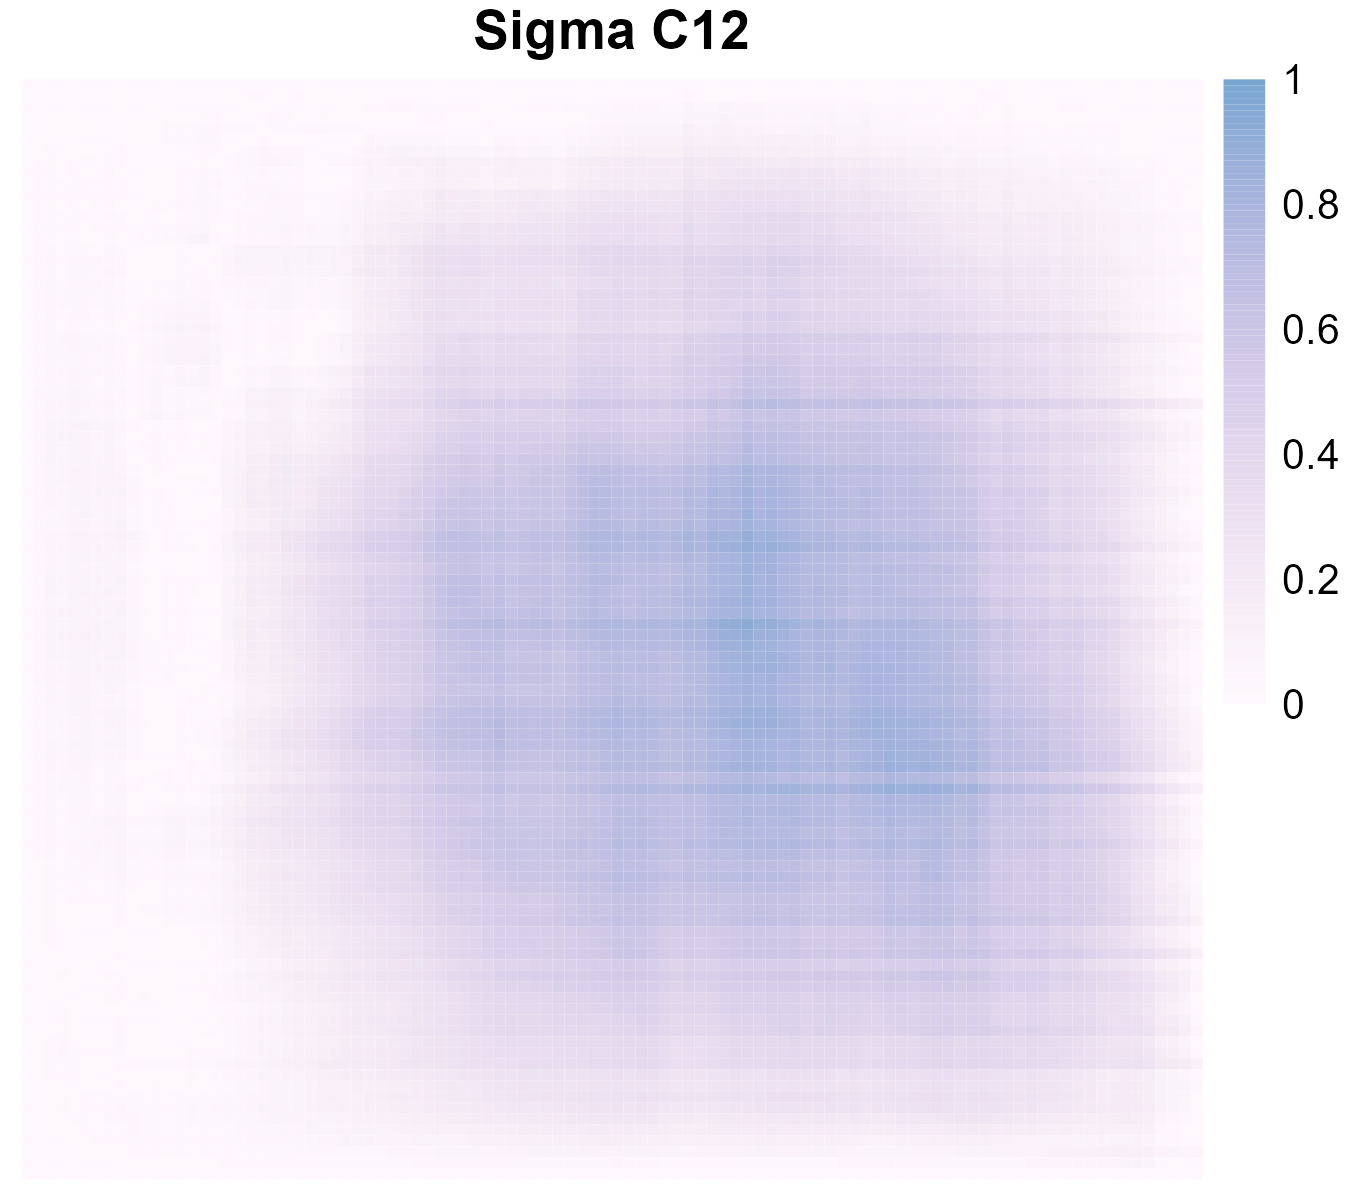
\includegraphics[width=0.33\textwidth]{4img/MujsigmaC12.png}}
  \subfloat[$\mathscr{H}_{C_{12}}$]{
   \label{C12H}
    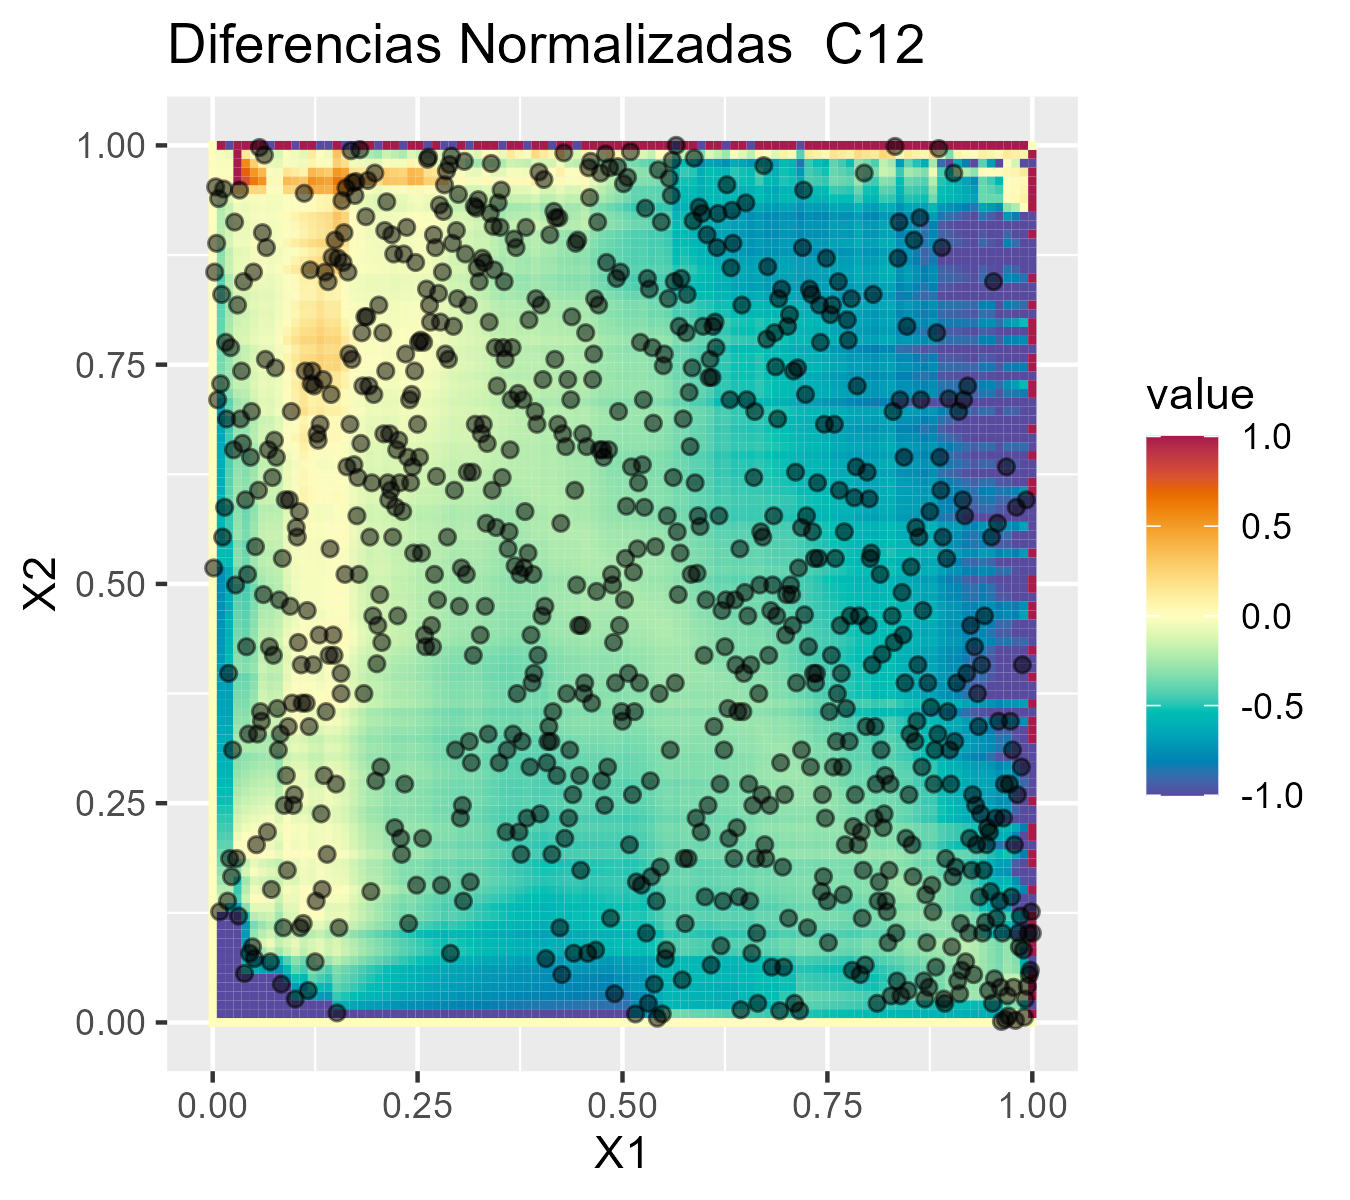
\includegraphics[width=0.33\textwidth]{4img/MujHC12.png}}
\end{figure}

\begin{figure}[H]
 \centering
  \subfloat[$\mathscr{H}\rho_{C_{23}}$]{
   \label{C23rho}
    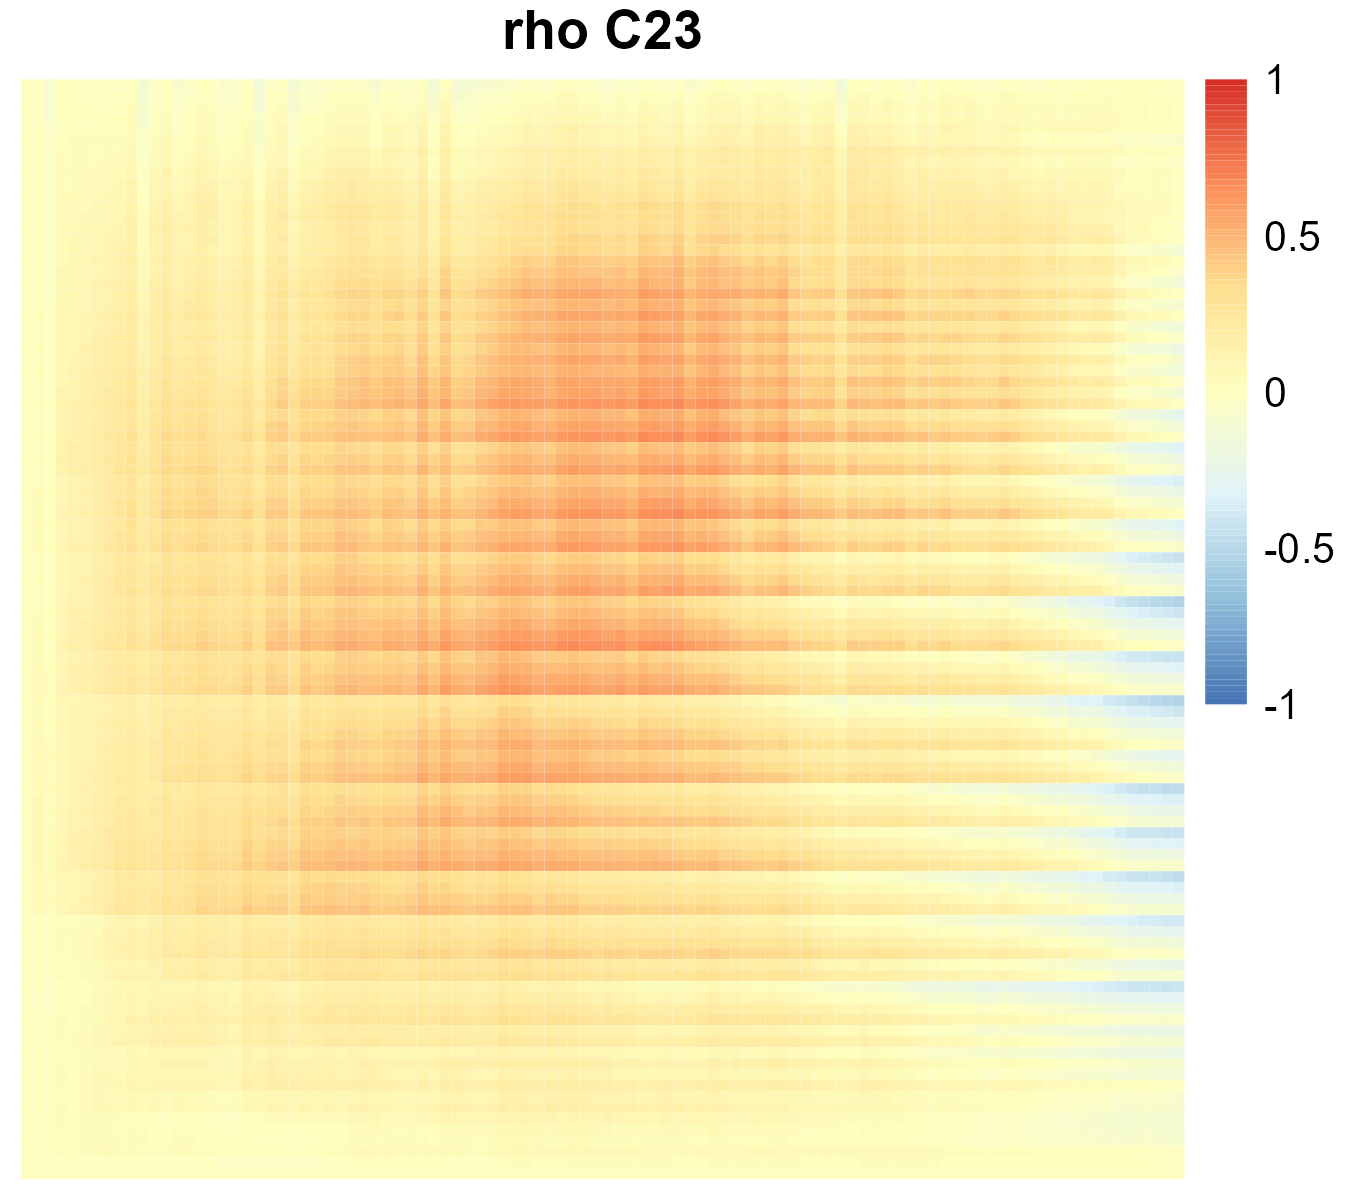
\includegraphics[width=0.33\textwidth]{4img/MujrhoC23.png}}
  \subfloat[$\mathscr{H}\sigma_{C_{23}}$]{
   \label{C23sigma}
    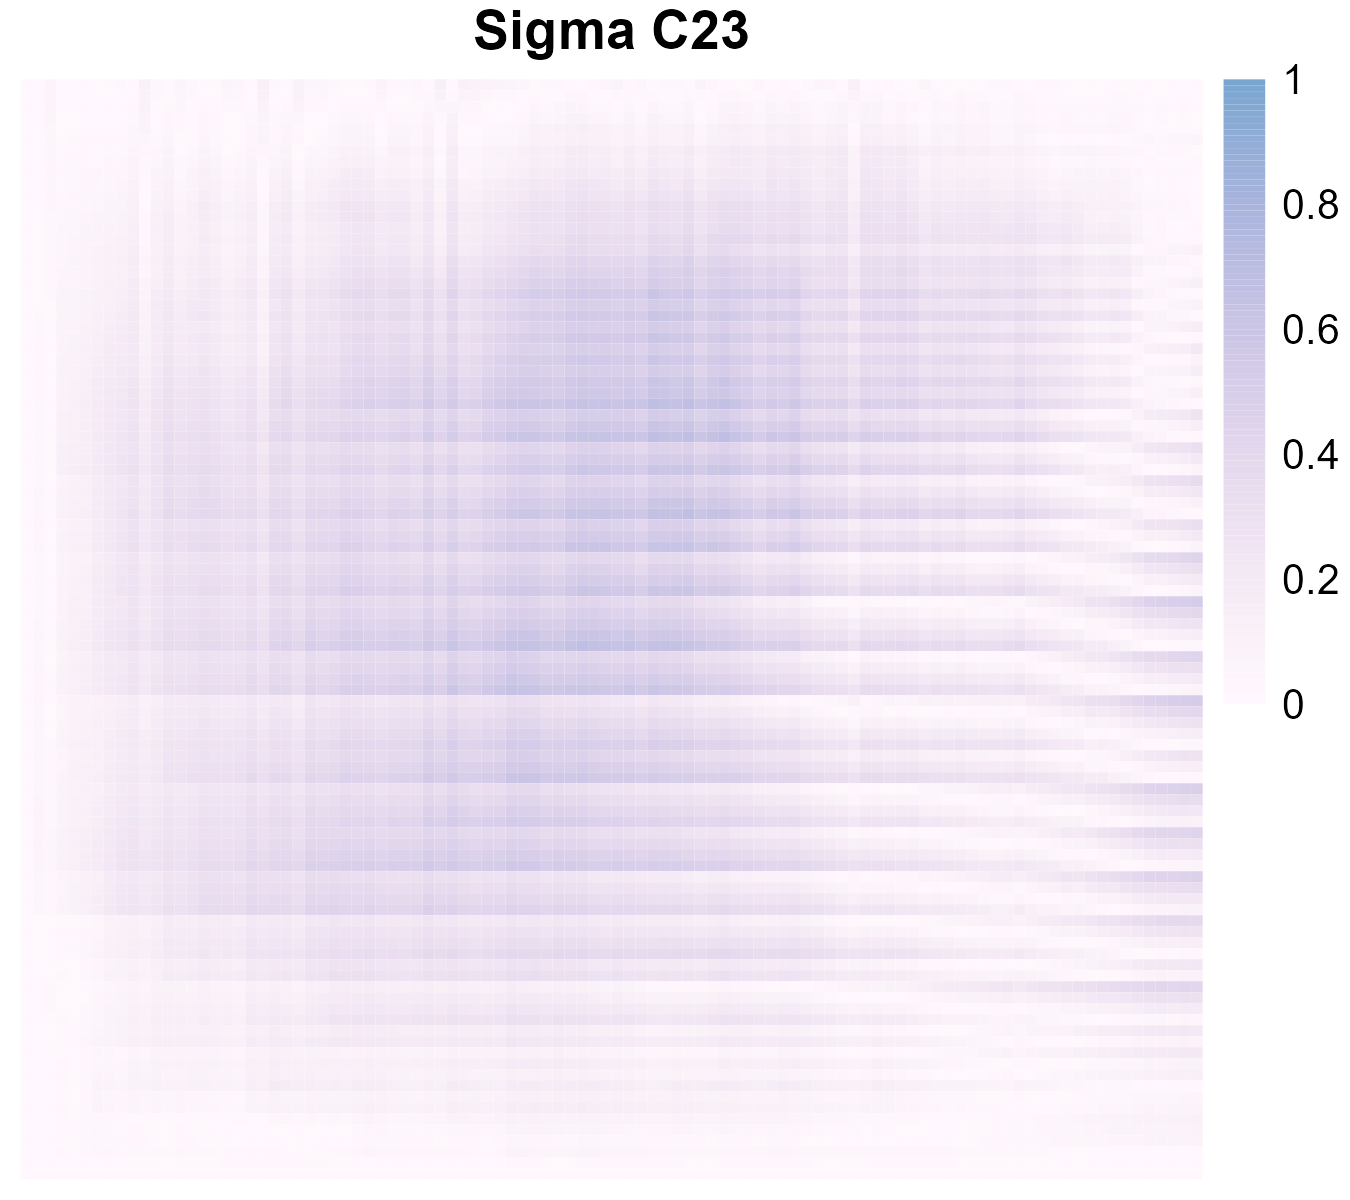
\includegraphics[width=0.33\textwidth]{4img/MujsigmaC23.png}}
  \subfloat[$\mathscr{H}_{C_{23}}$]{
   \label{C23H}
    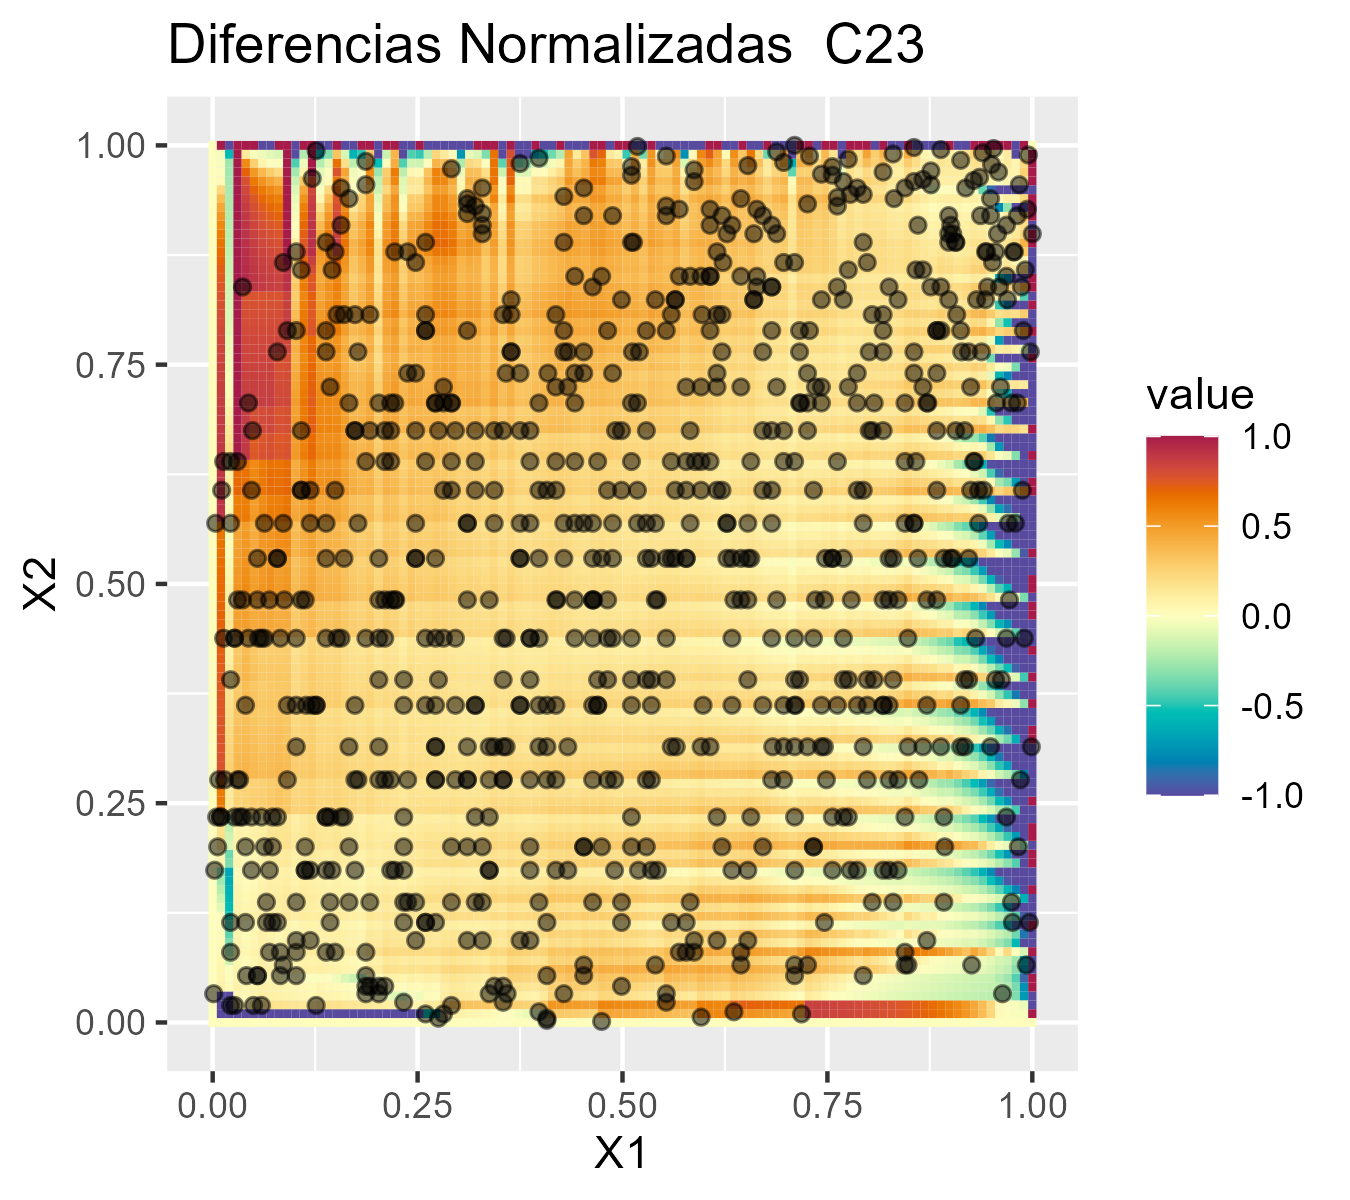
\includegraphics[width=0.33\textwidth]{4img/MujHC23.png}}
\end{figure}

\begin{figure}[H]
 \centering
  \subfloat[$\mathscr{H}\rho_{C_{34}}$]{
   \label{C34rho}
    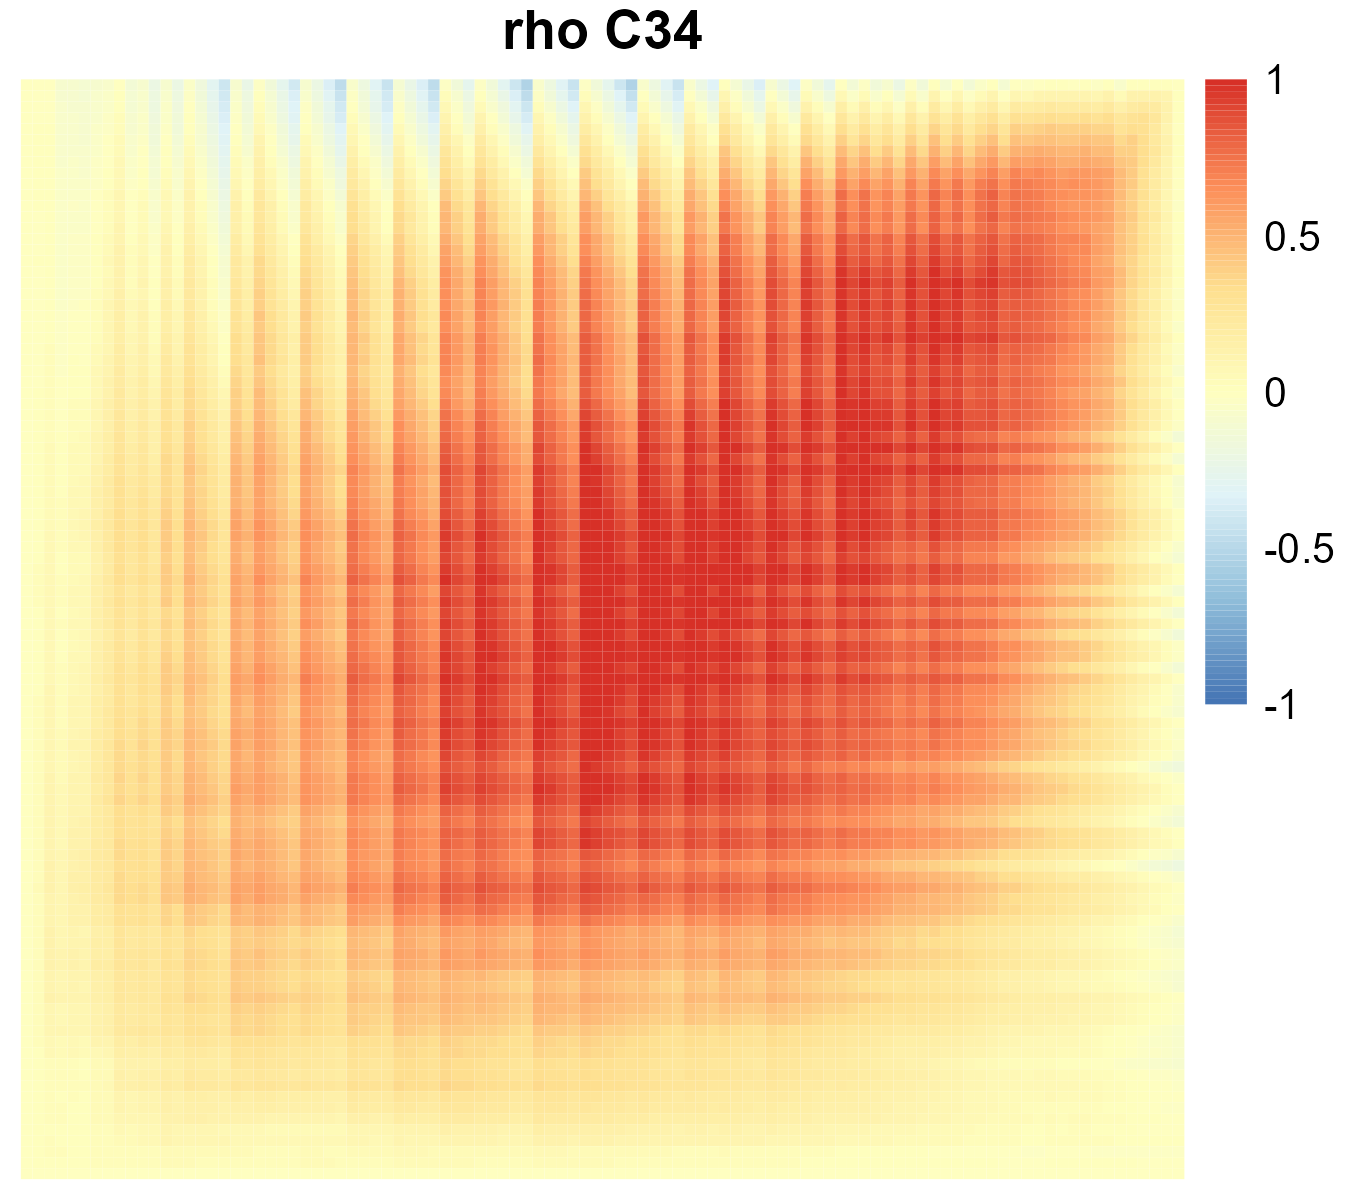
\includegraphics[width=0.33\textwidth]{4img/MujrhoC34.png}}
  \subfloat[$\mathscr{H}\sigma_{C_{34}}$]{
   \label{C34sigma}
    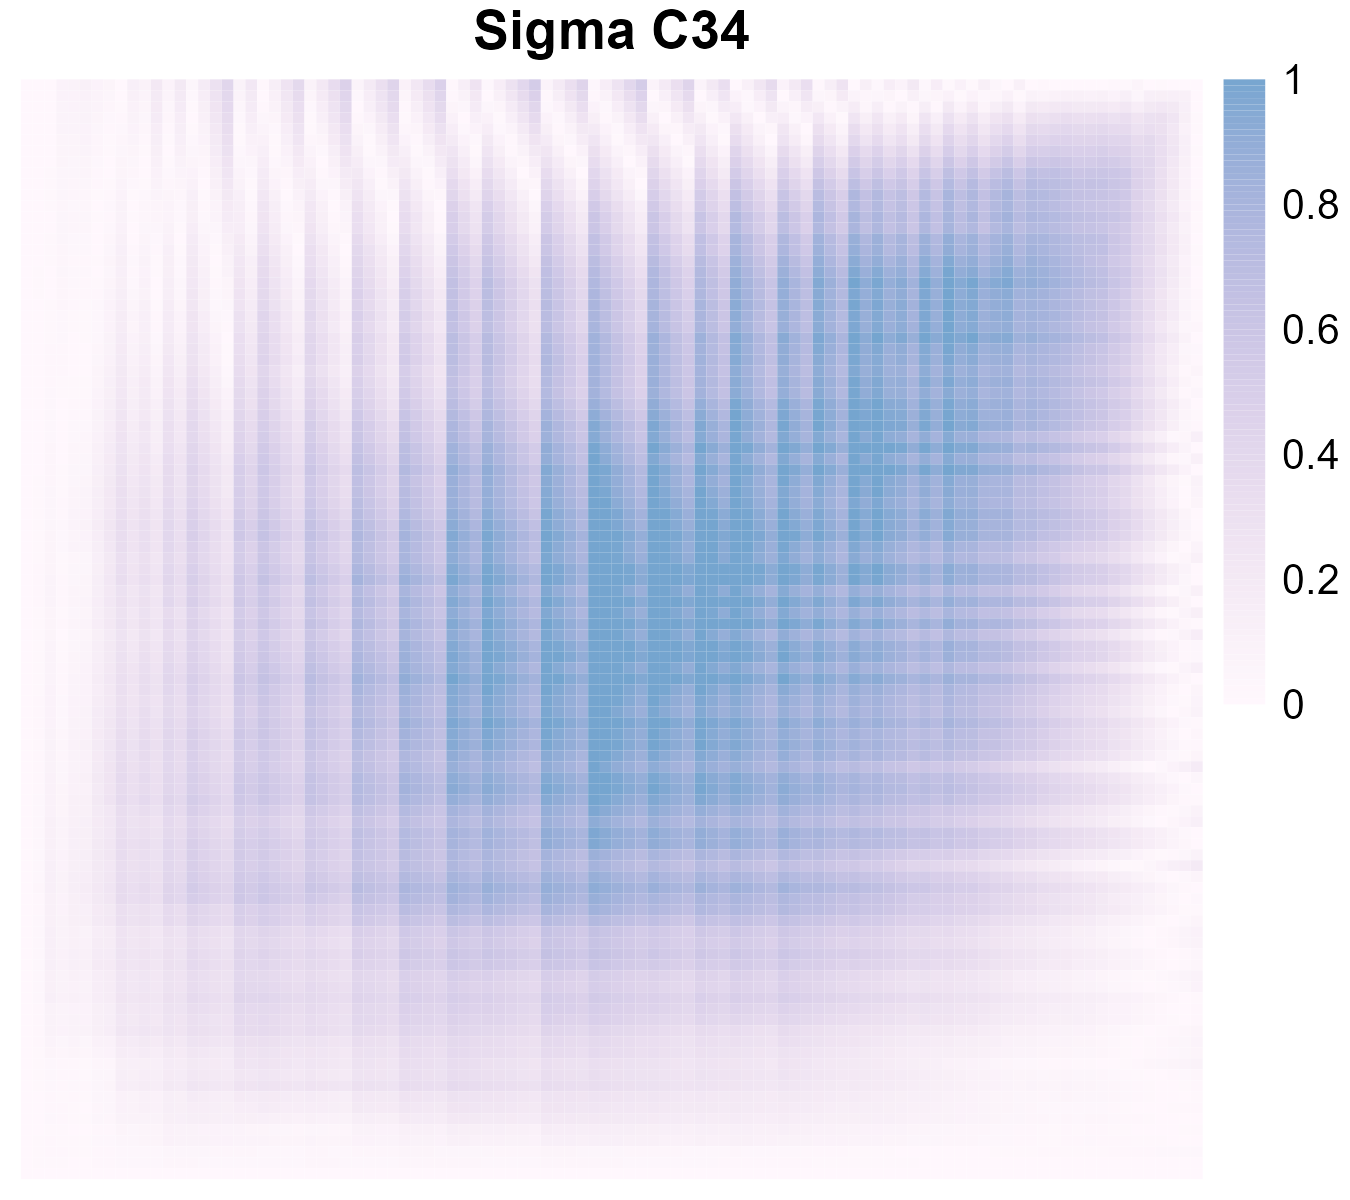
\includegraphics[width=0.33\textwidth]{4img/MujsigmaC34.png}}
  \subfloat[$\mathscr{H}_{C_{34}}$]{
   \label{C34H}
    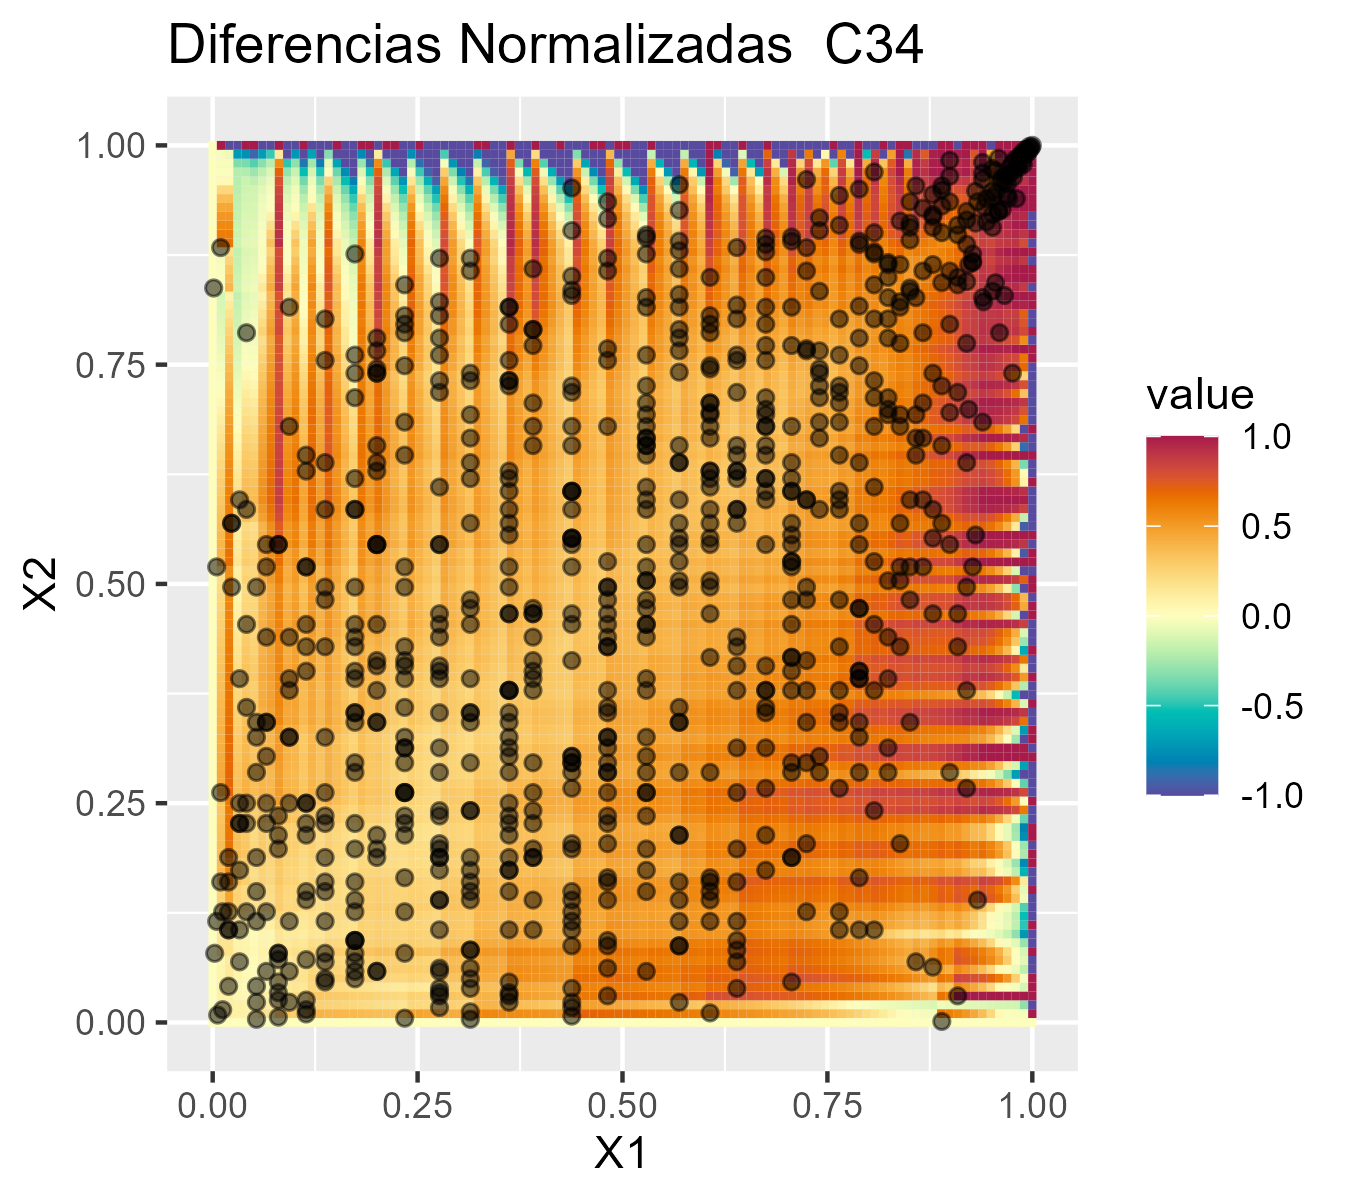
\includegraphics[width=0.33\textwidth]{4img/MujHC34.png}}
\end{figure}

\begin{figure}[H]
 \centering
  \subfloat[$\mathscr{H}\rho_{C_{45}}$]{
   \label{C45rho}
    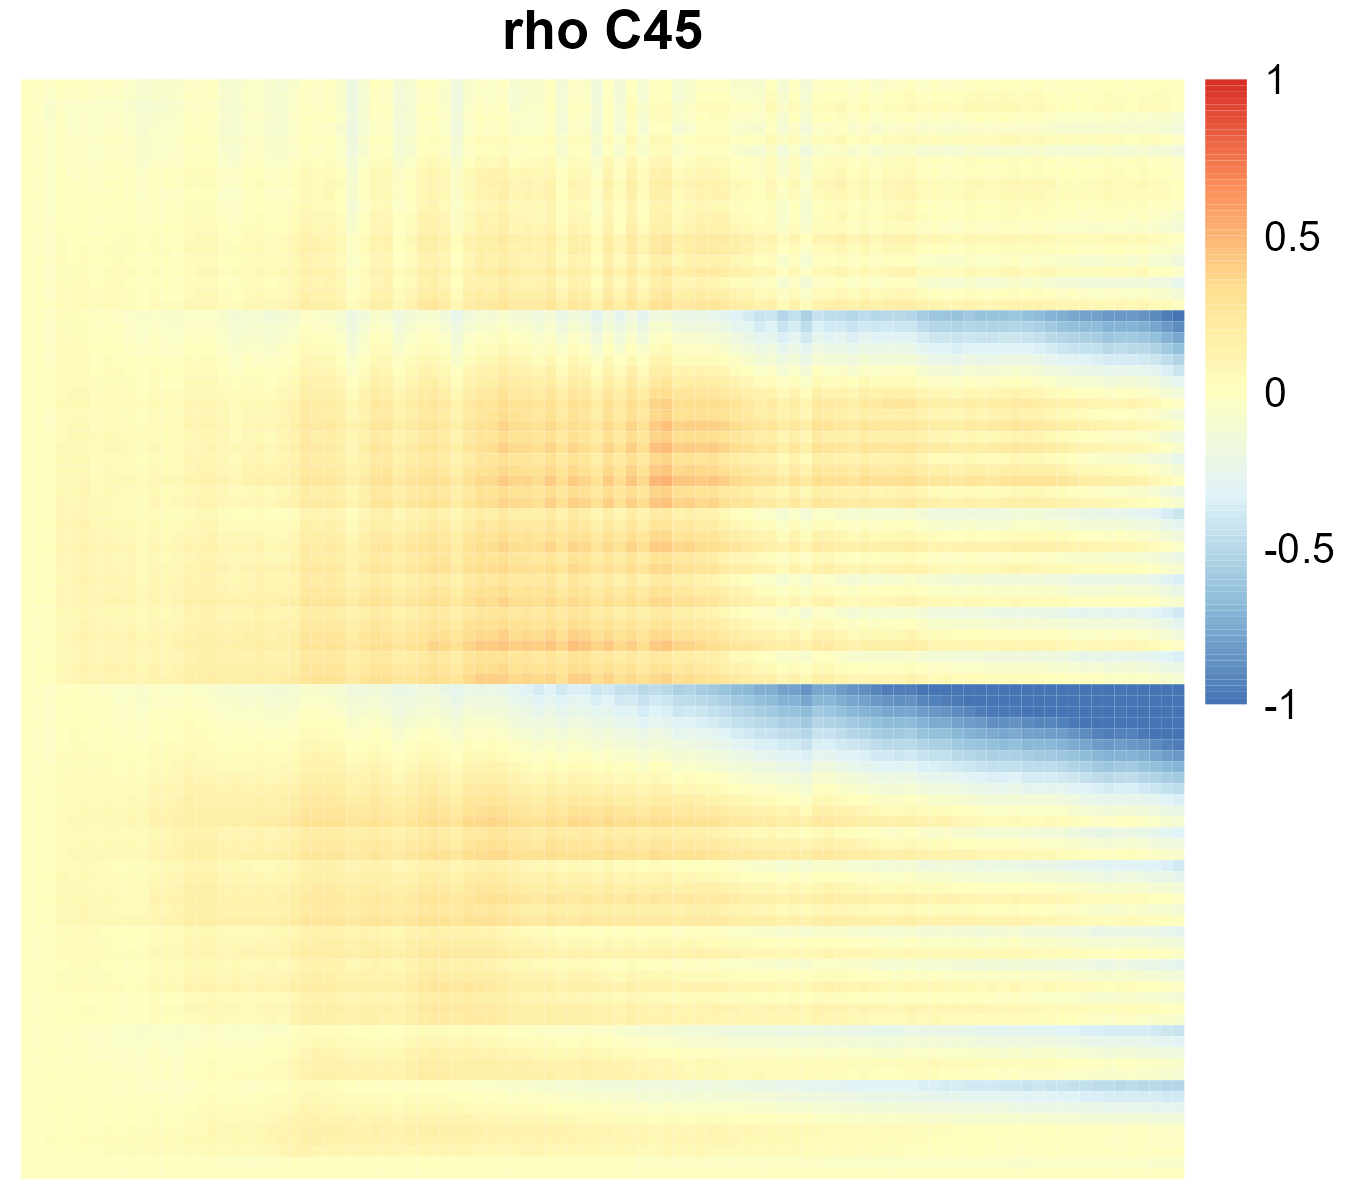
\includegraphics[width=0.33\textwidth]{4img/MujrhoC45.png}}
  \subfloat[$\mathscr{H}\sigma_{C_{45}}$]{
   \label{C45sigma}
    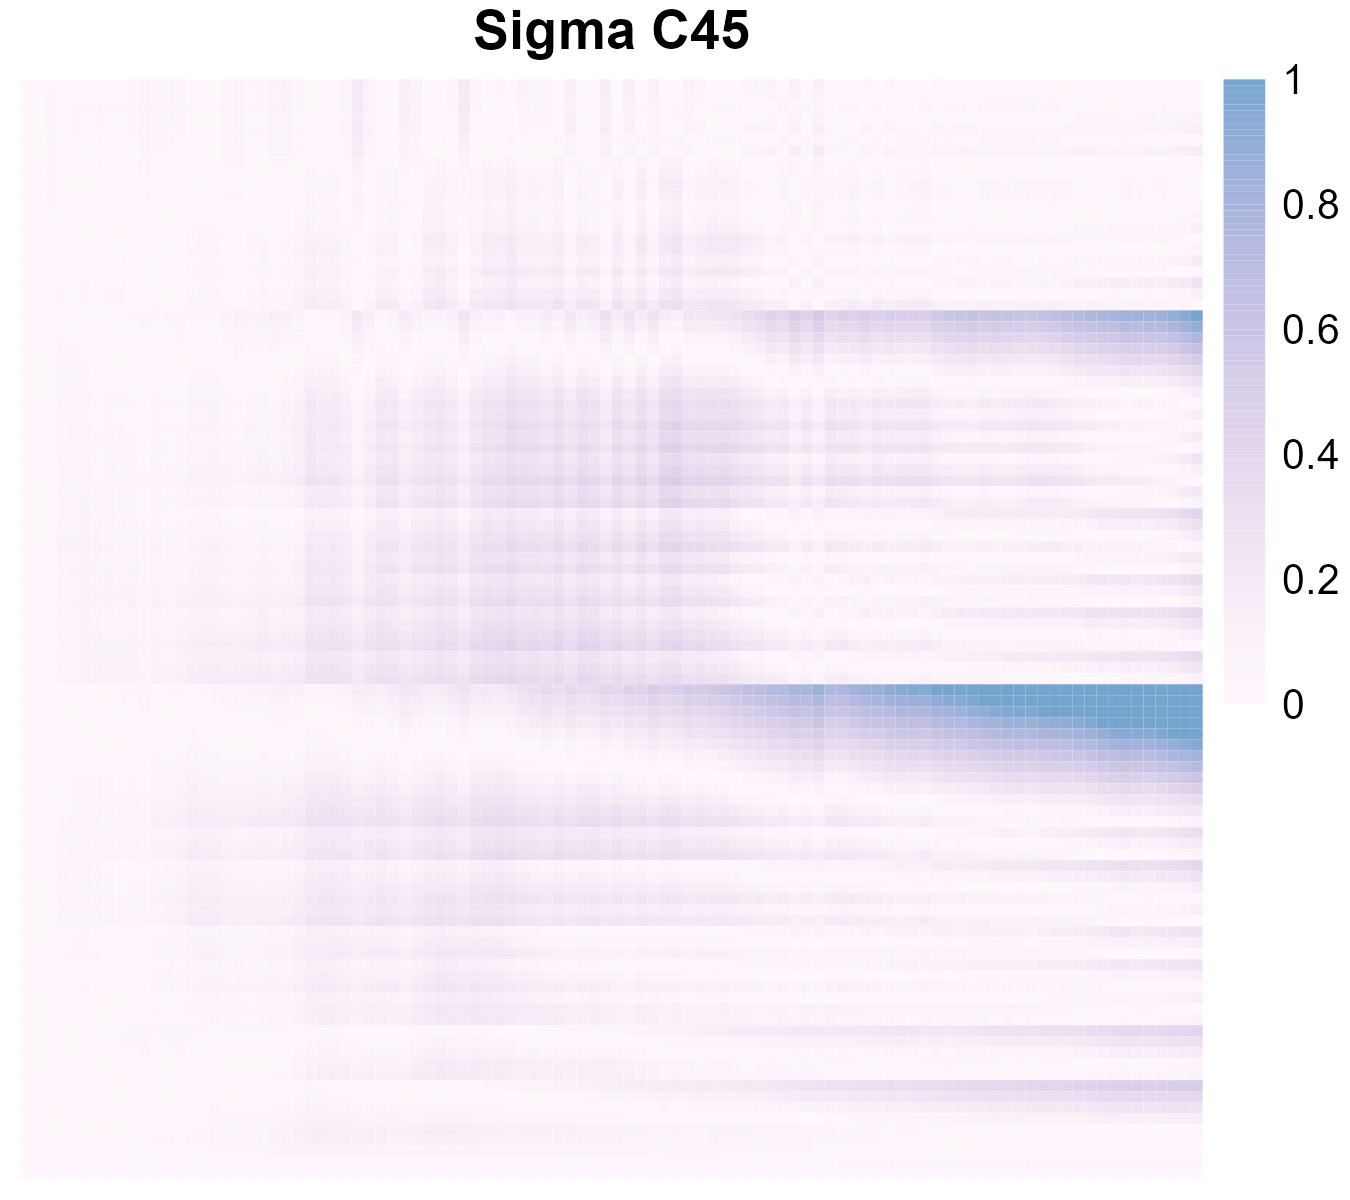
\includegraphics[width=0.33\textwidth]{4img/MujsigmaC45.png}}
  \subfloat[$\mathscr{H}_{C_{45}}$]{
   \label{C45H}
    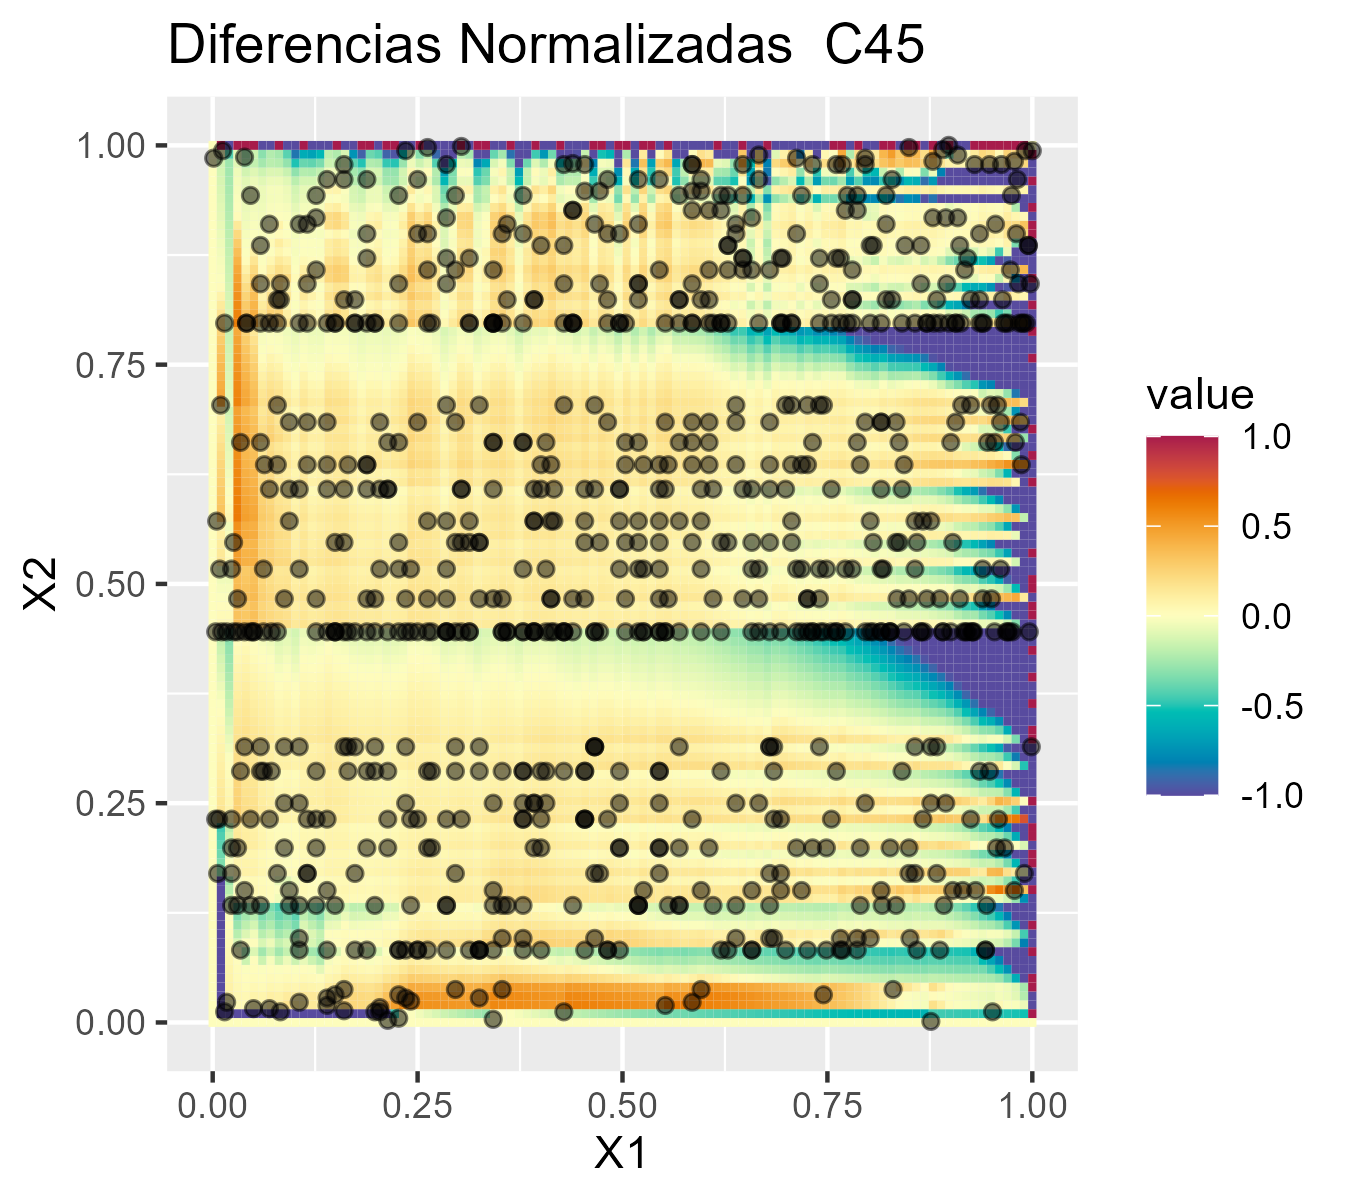
\includegraphics[width=0.33\textwidth]{4img/MujHC45.png}}
    \caption{Cópulas ajustadas para mujeres, nivel $1$.}
    \label{fig:Modelo4MujNivel1}
\end{figure}

%%%%%%%%%%%%%%%%%%%%%%%%%%%%%%%%%%%%%%%%%%%%%%%%%%

\begin{figure}[H]
 \centering
  \subfloat[$\mathscr{H}\rho_{C_{13|2}}$]{
   \label{C13.2rho}
    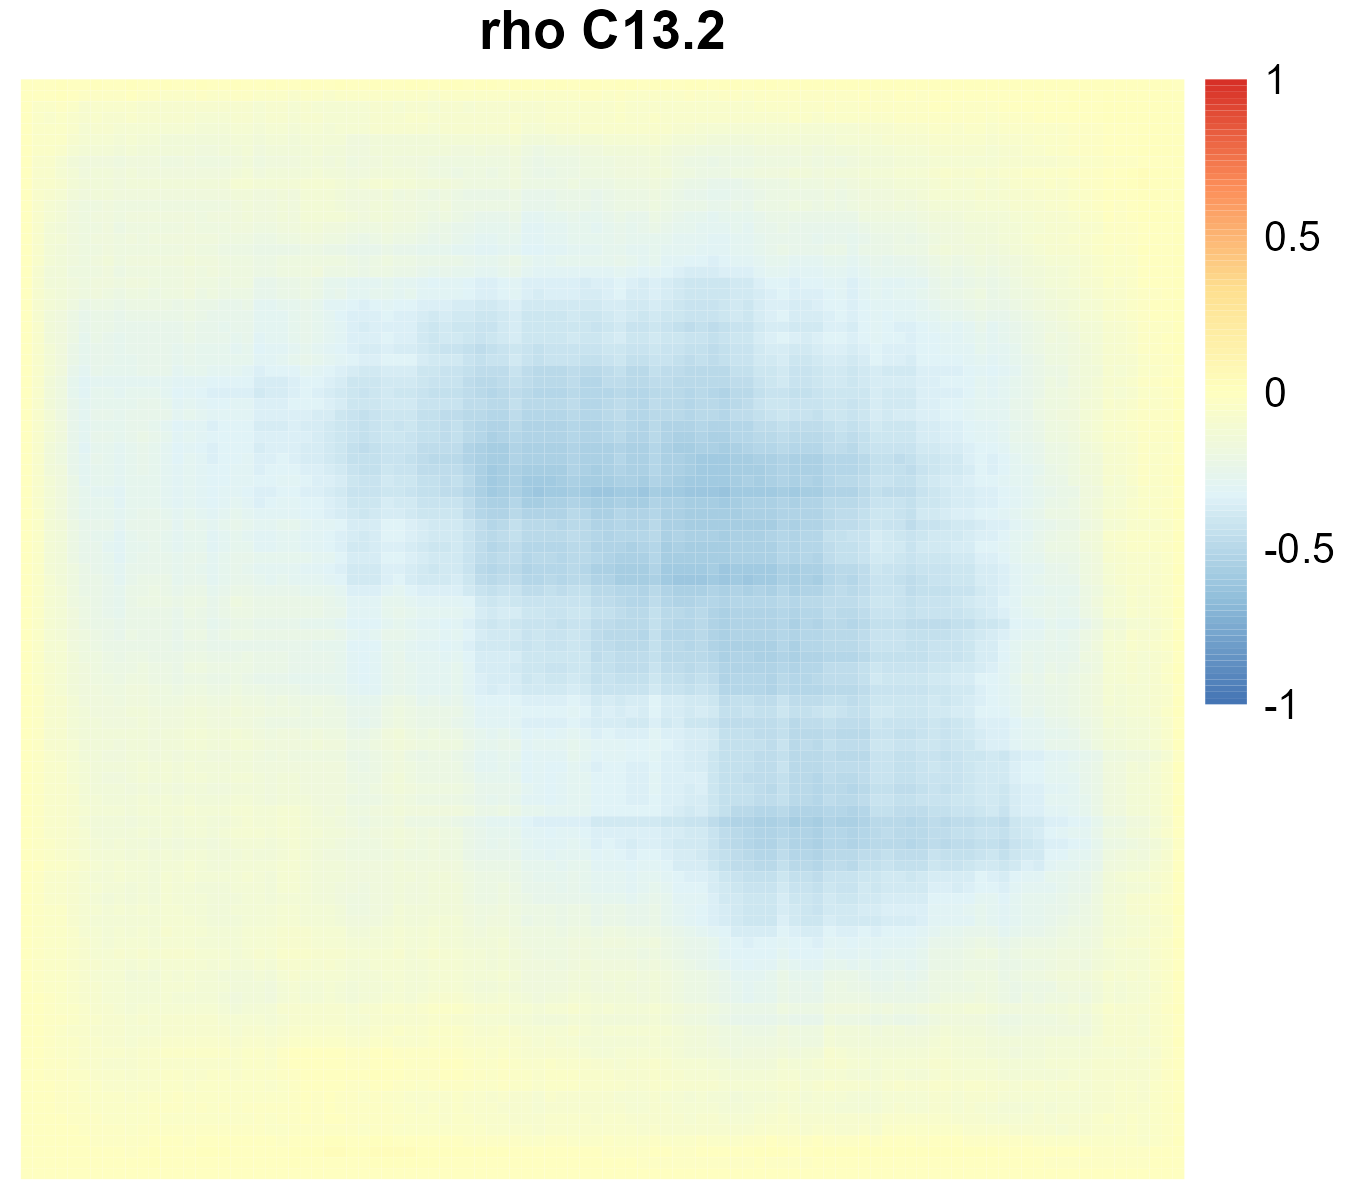
\includegraphics[width=0.33\textwidth]{4img/MujrhoC13.2.png}}
  \subfloat[$\mathscr{H}\sigma_{C_{13|2}}$]{
   \label{C13.2sigma}
    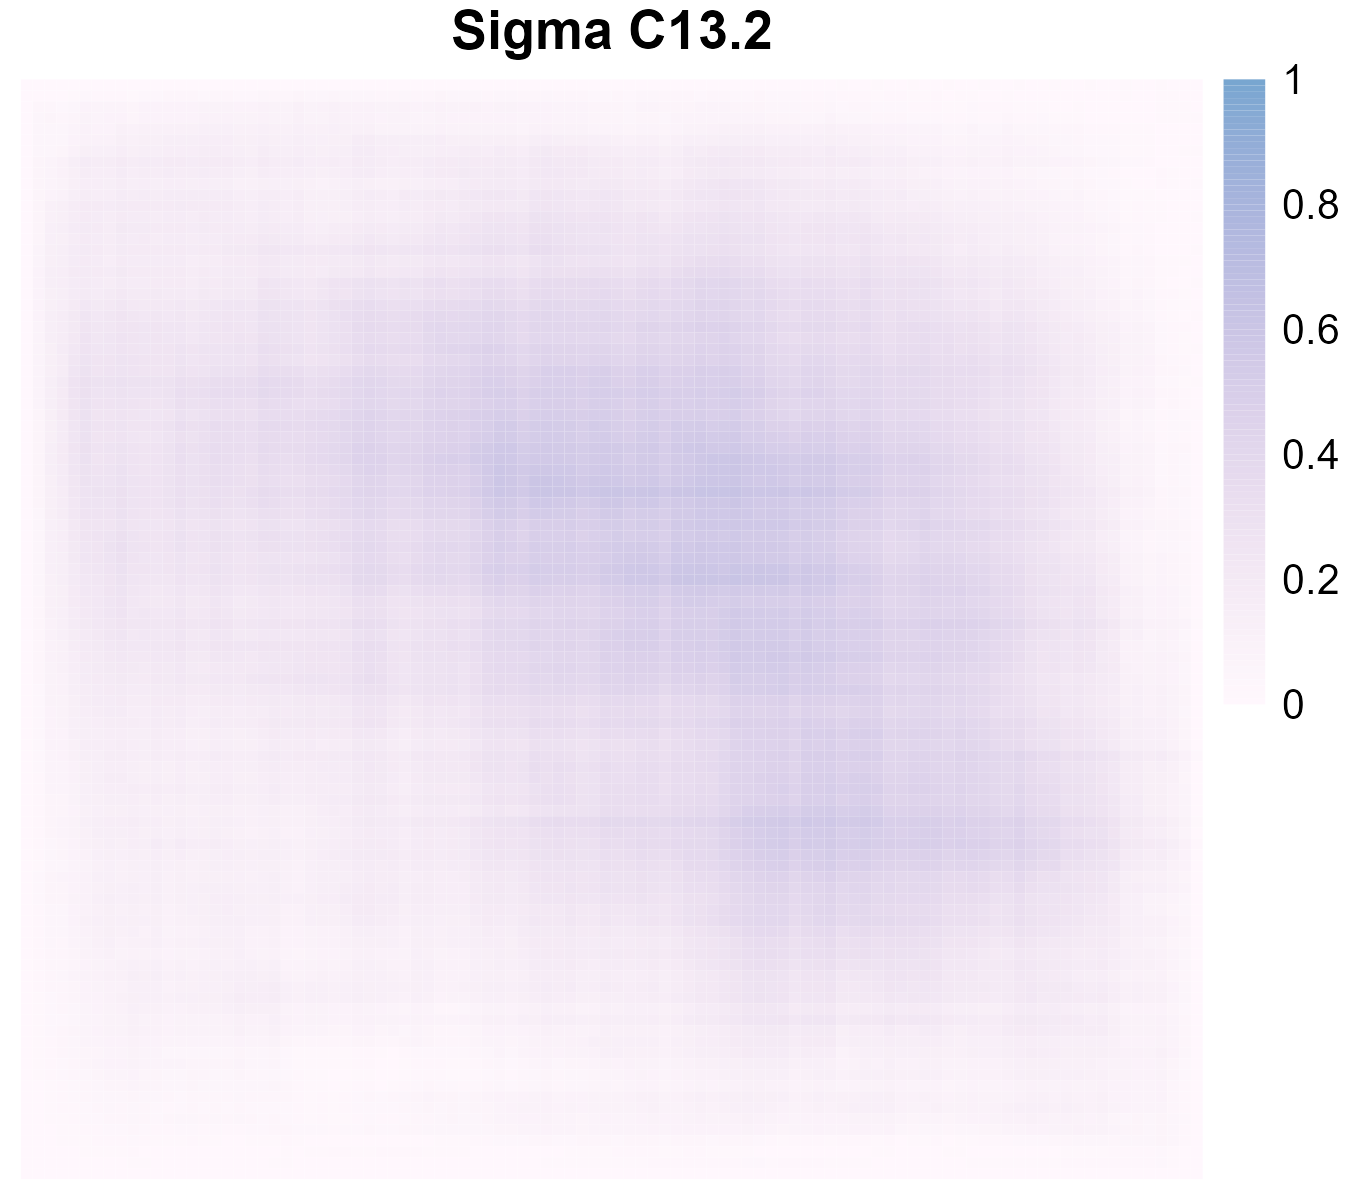
\includegraphics[width=0.33\textwidth]{4img/MujsigmaC13.2.png}}
  \subfloat[$\mathscr{H}_{C_{13|2}}$]{
   \label{C13.2H}
    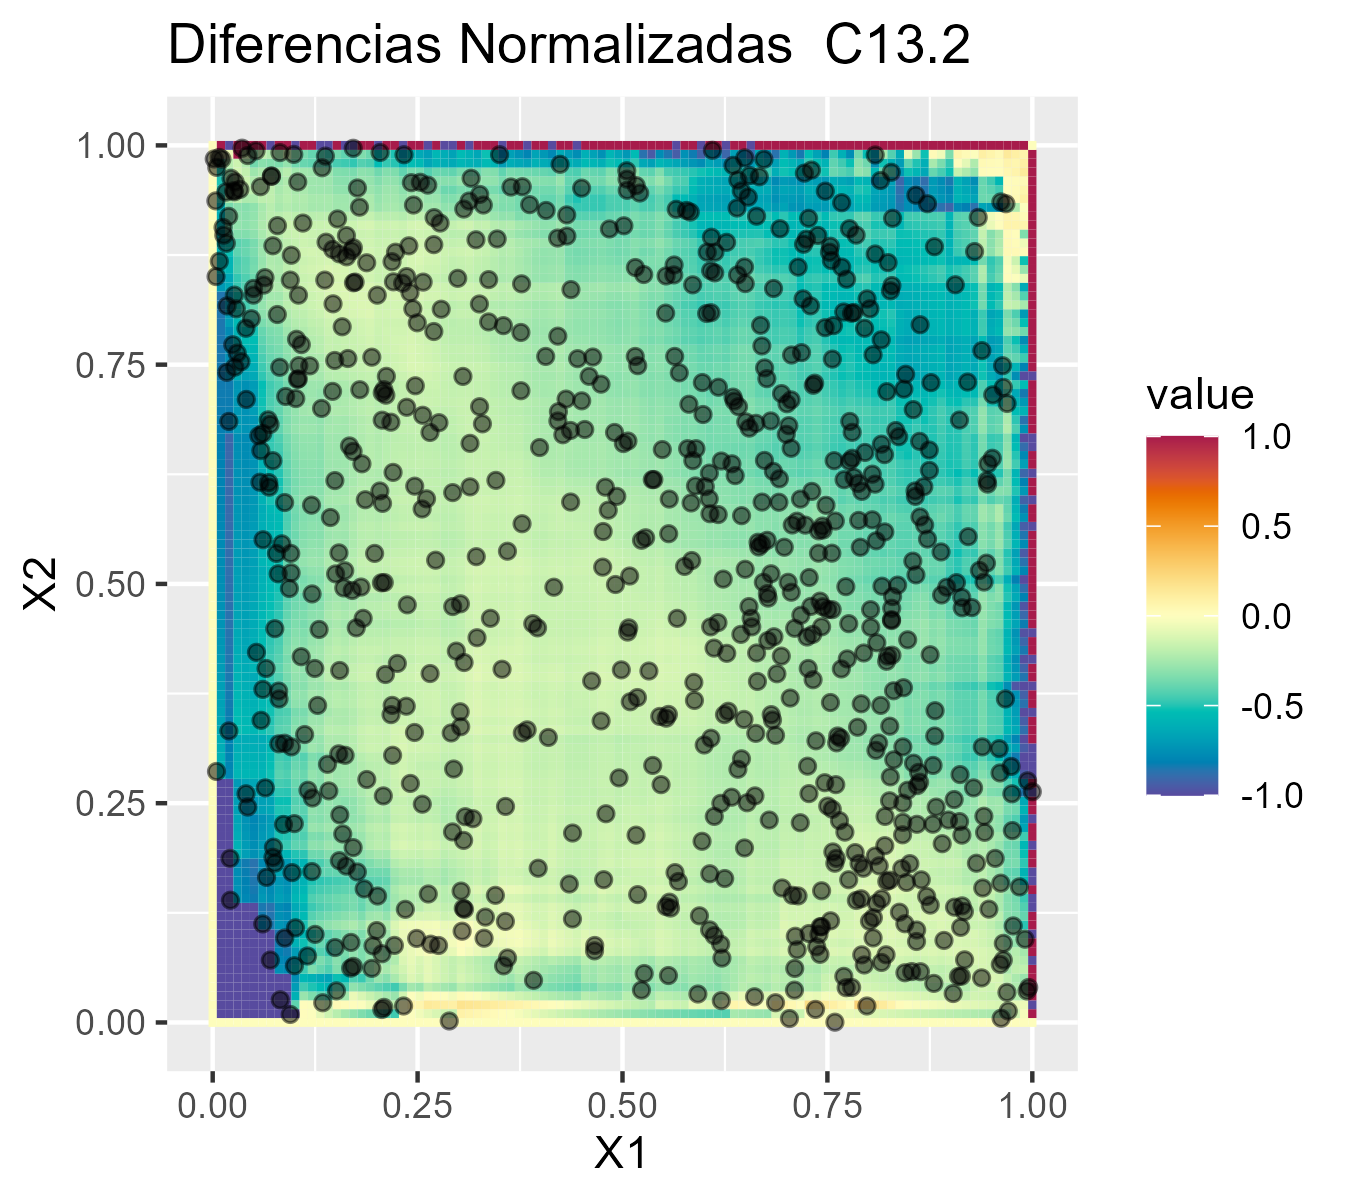
\includegraphics[width=0.33\textwidth]{4img/MujHC13.2.png}}
\end{figure}

\begin{figure}[H]
 \centering
  \subfloat[$\mathscr{H}\rho_{C_{24|3}}$]{
   \label{C24.3rho}
    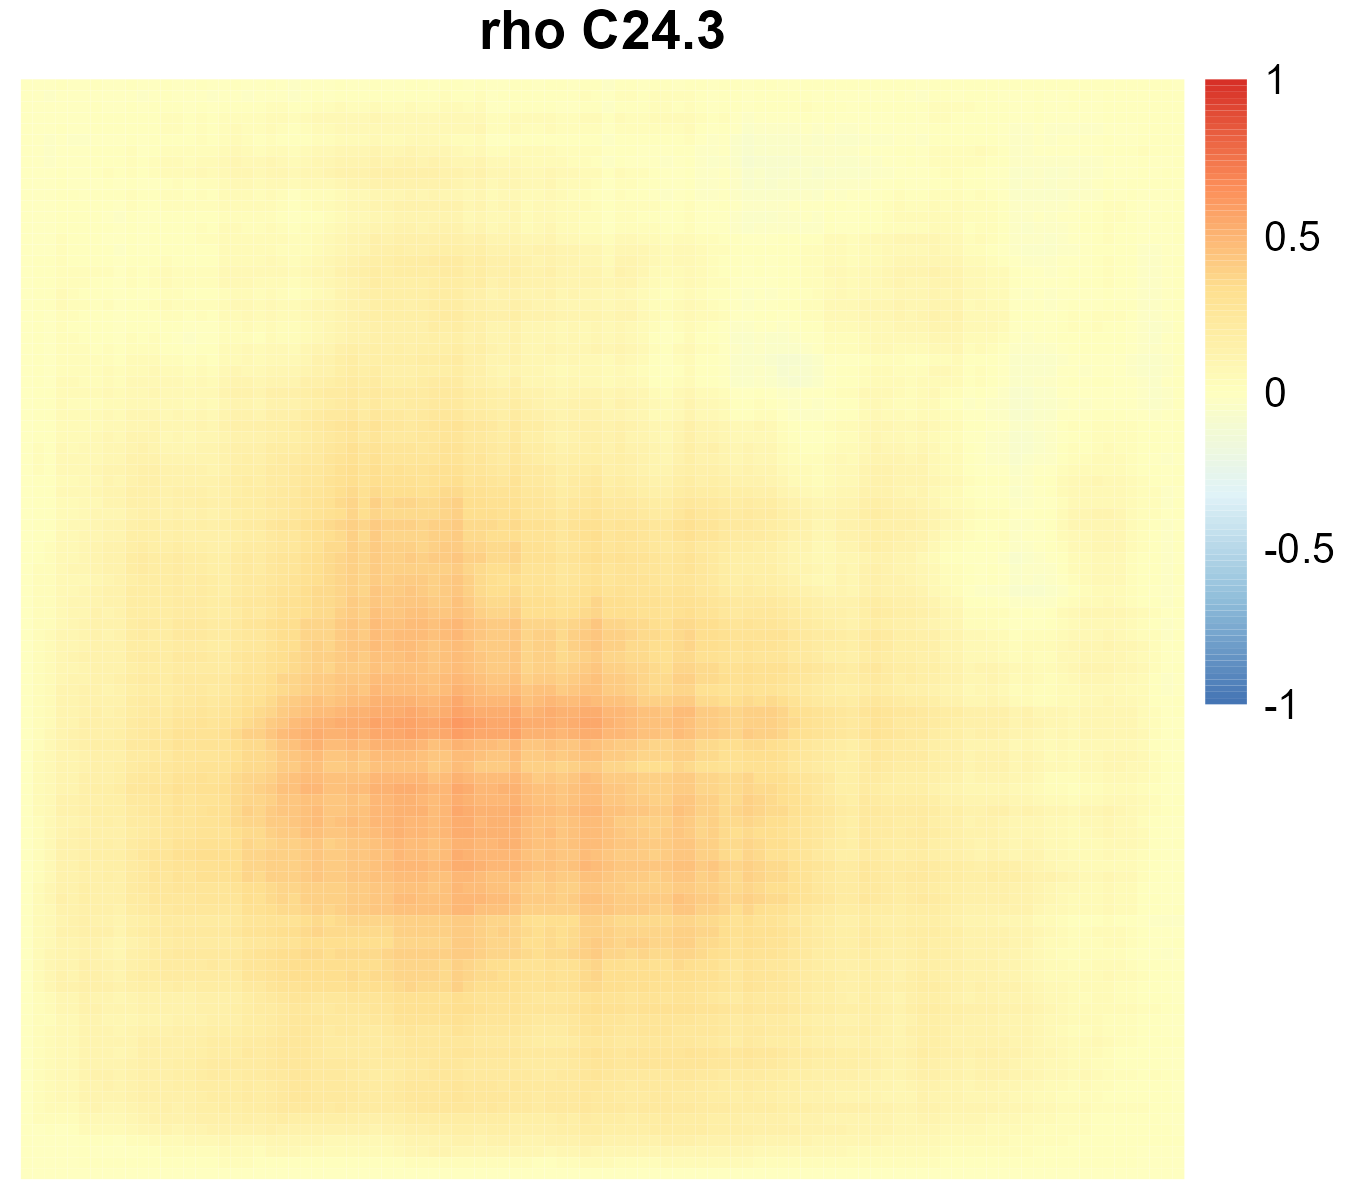
\includegraphics[width=0.33\textwidth]{4img/MujrhoC24.3.png}}
  \subfloat[$\mathscr{H}\sigma_{C_{24|3}}$]{
   \label{C24.3sigma}
    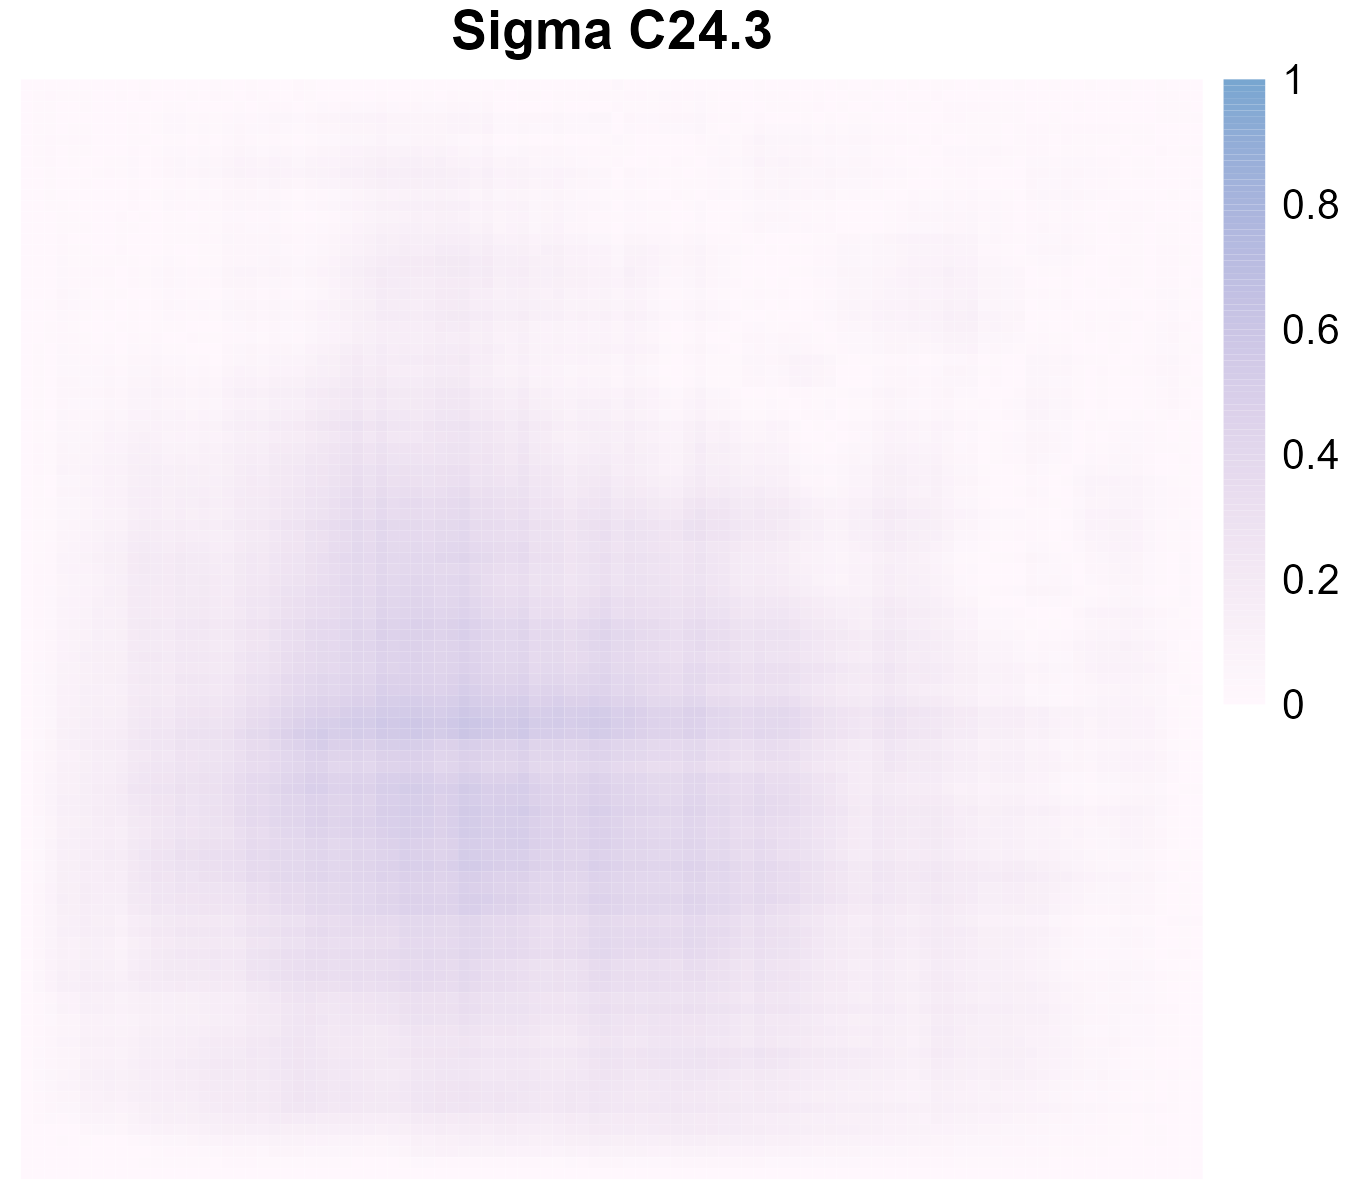
\includegraphics[width=0.33\textwidth]{4img/MujsigmaC24.3.png}}
  \subfloat[$\mathscr{H}_{C_{24|3}}$]{
   \label{C24.3H}
    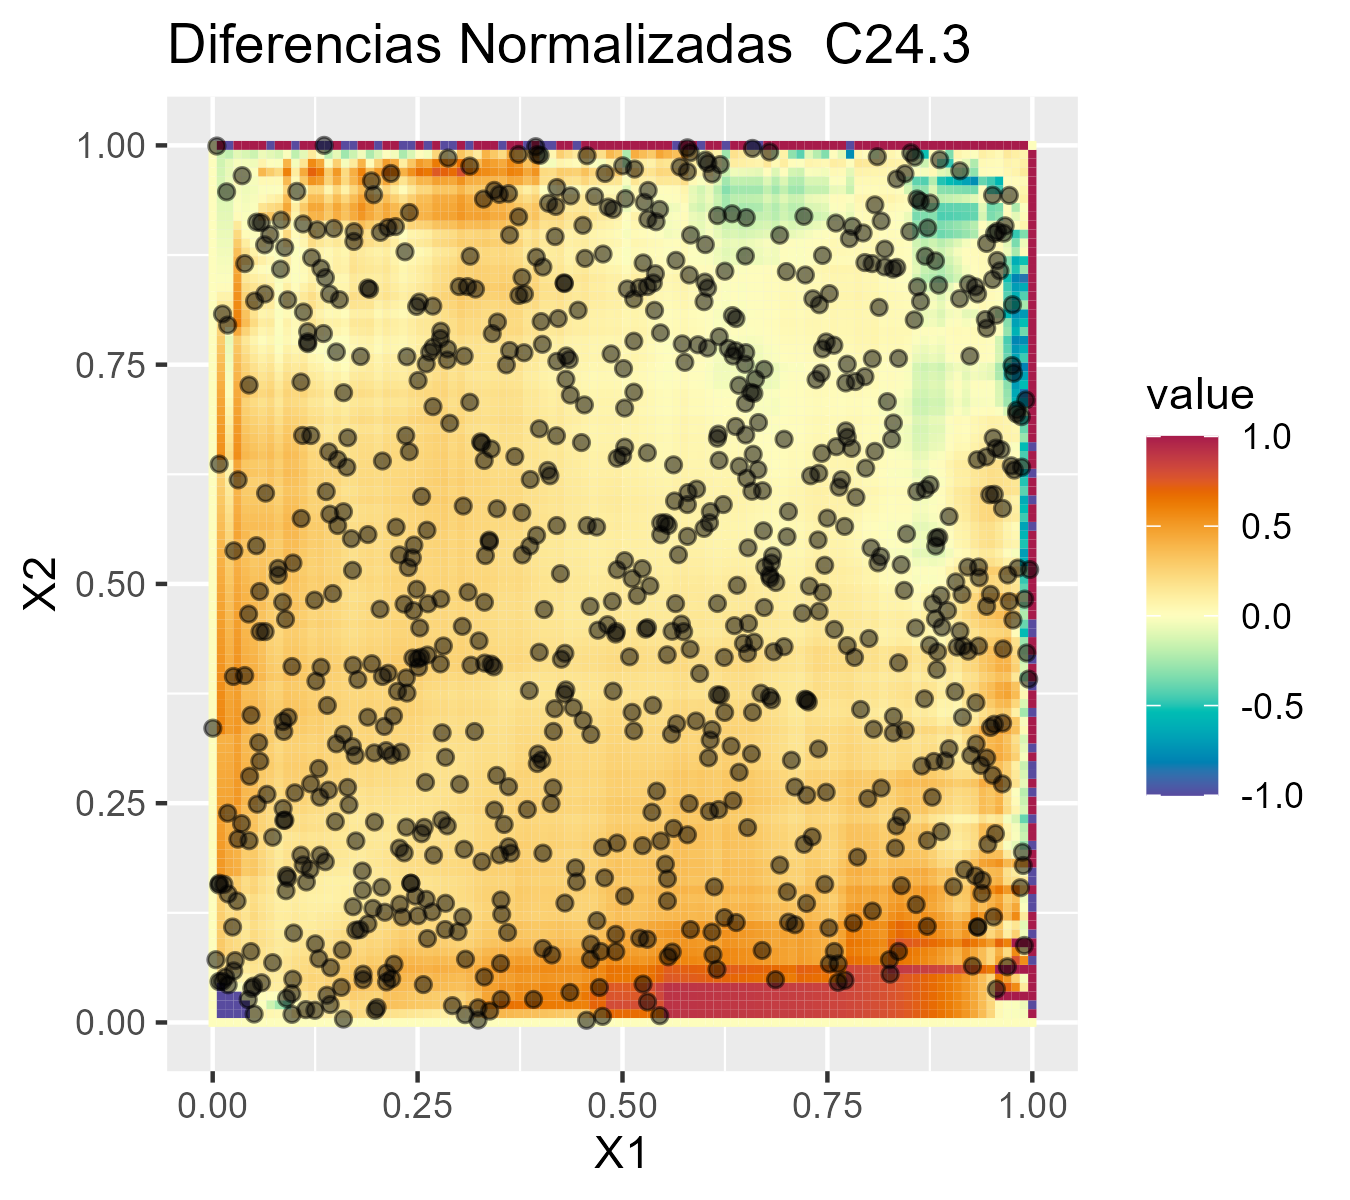
\includegraphics[width=0.33\textwidth]{4img/MujHC24.3.png}}
\end{figure}

\begin{figure}[H]
 \centering
  \subfloat[$\mathscr{H}\rho_{C_{35|4}}$]{
   \label{C35.4rho}
    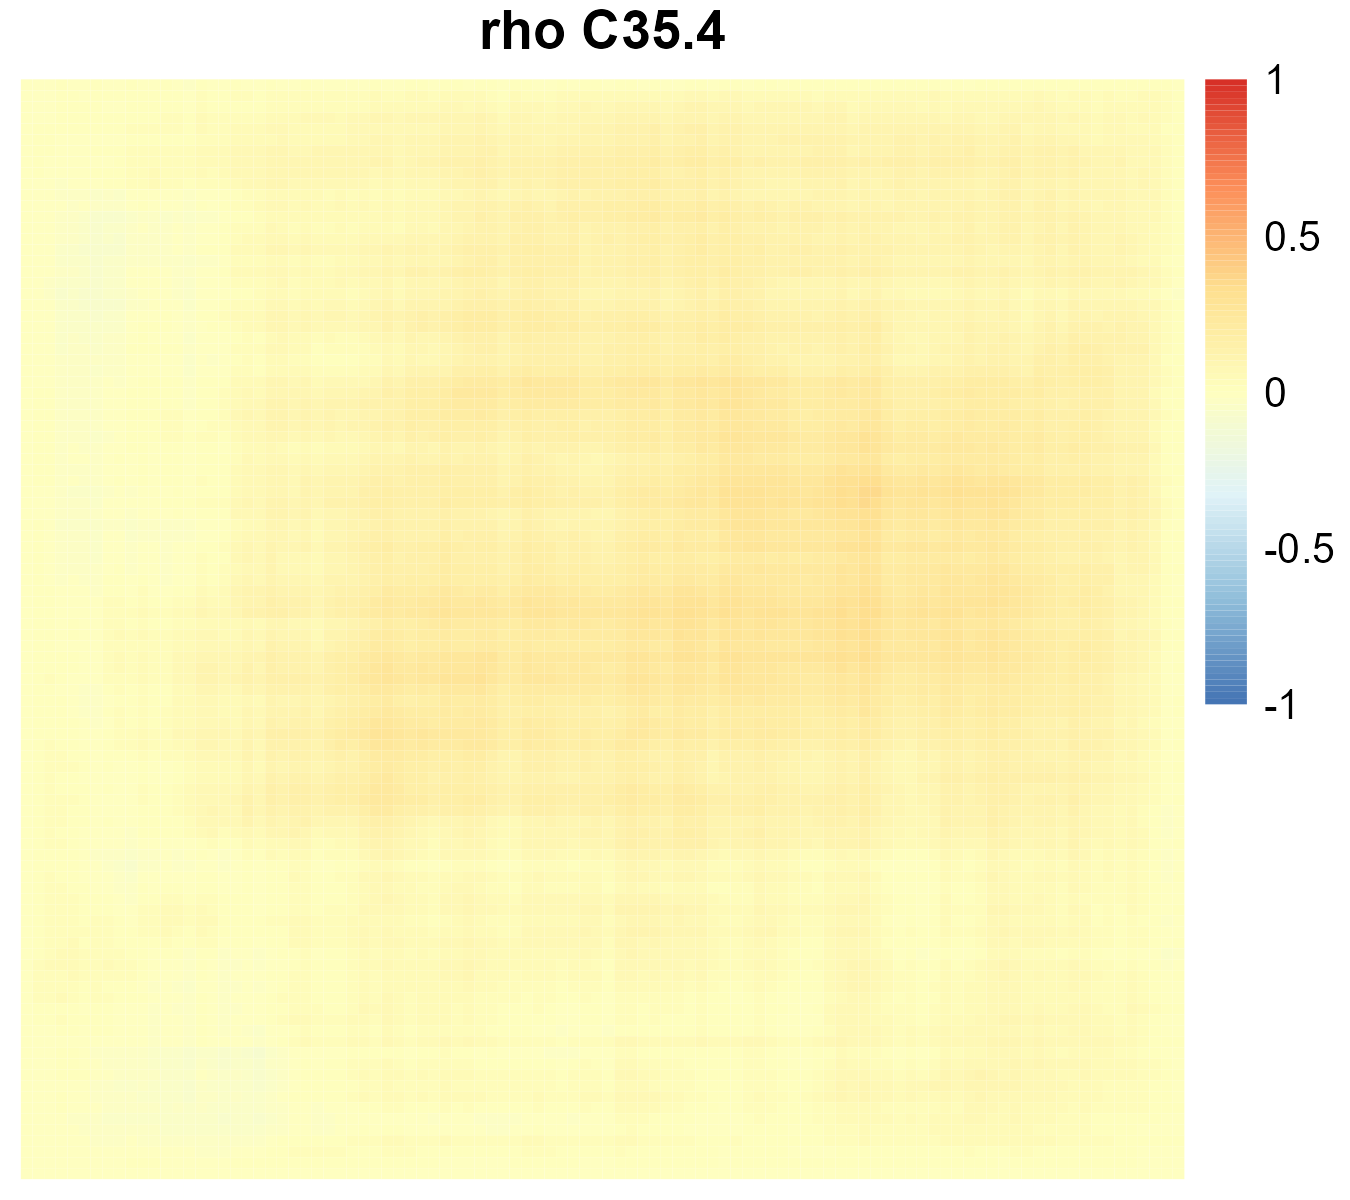
\includegraphics[width=0.33\textwidth]{4img/MujrhoC35.4.png}}
  \subfloat[$\mathscr{H}\sigma_{C_{35|4}}$]{
   \label{C35.4sigma}
    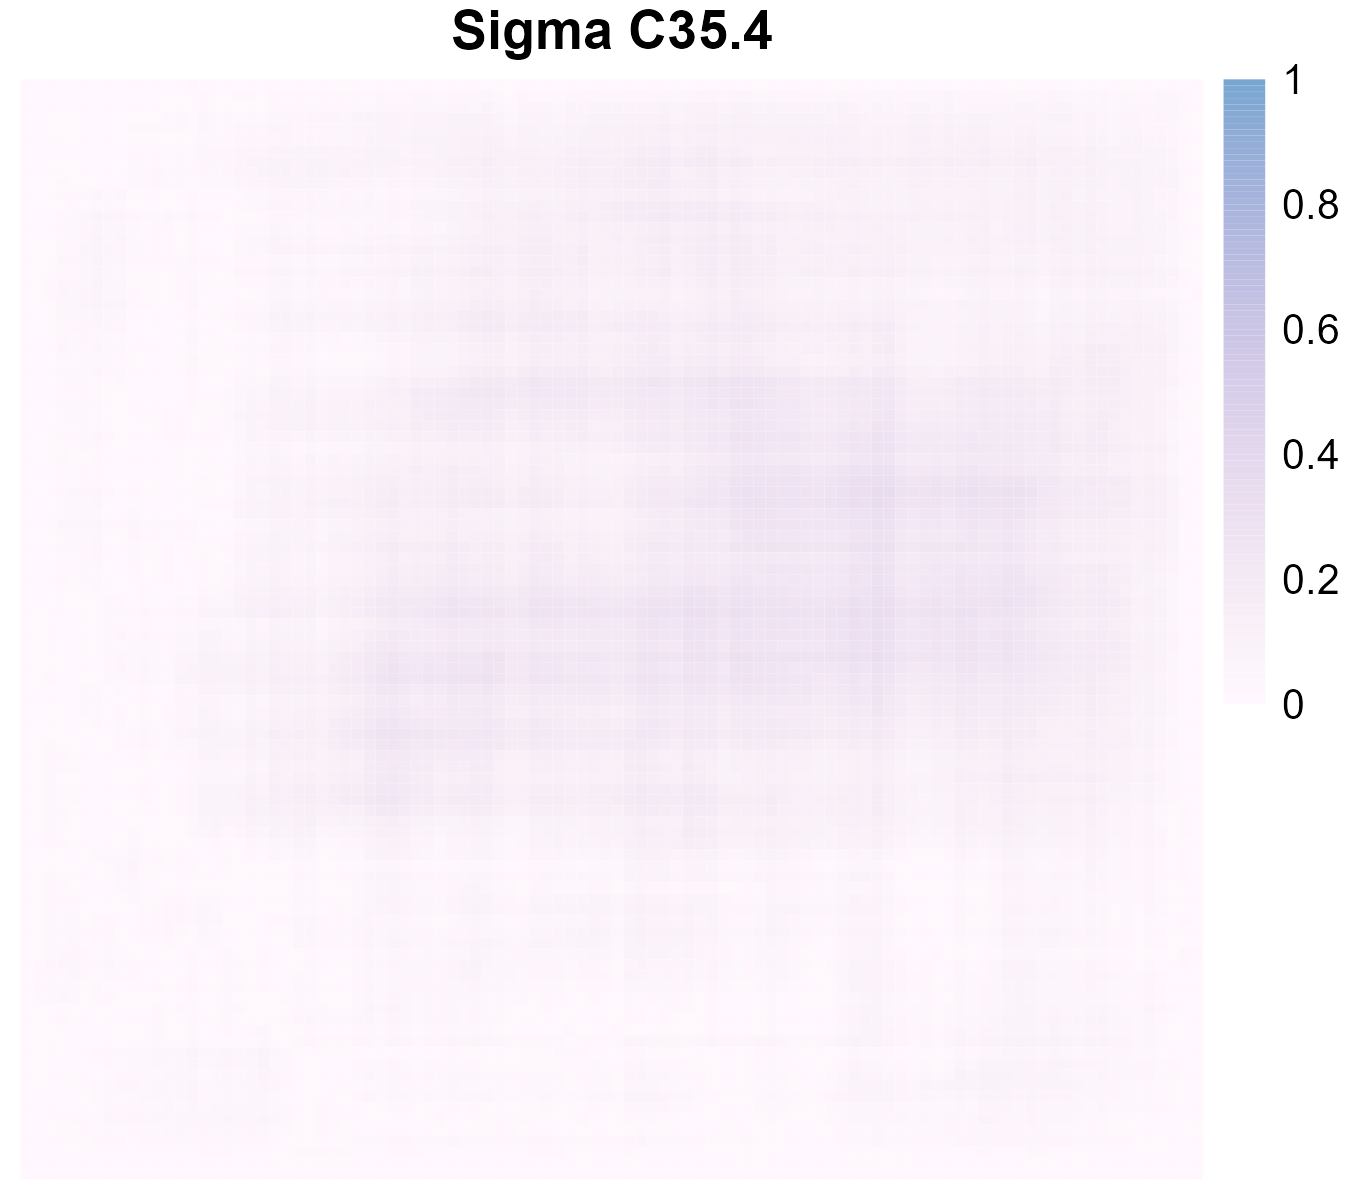
\includegraphics[width=0.33\textwidth]{4img/MujsigmaC35.4.png}}
  \subfloat[$\mathscr{H}_{C_{35|4}}$]{
   \label{C35.4H}
    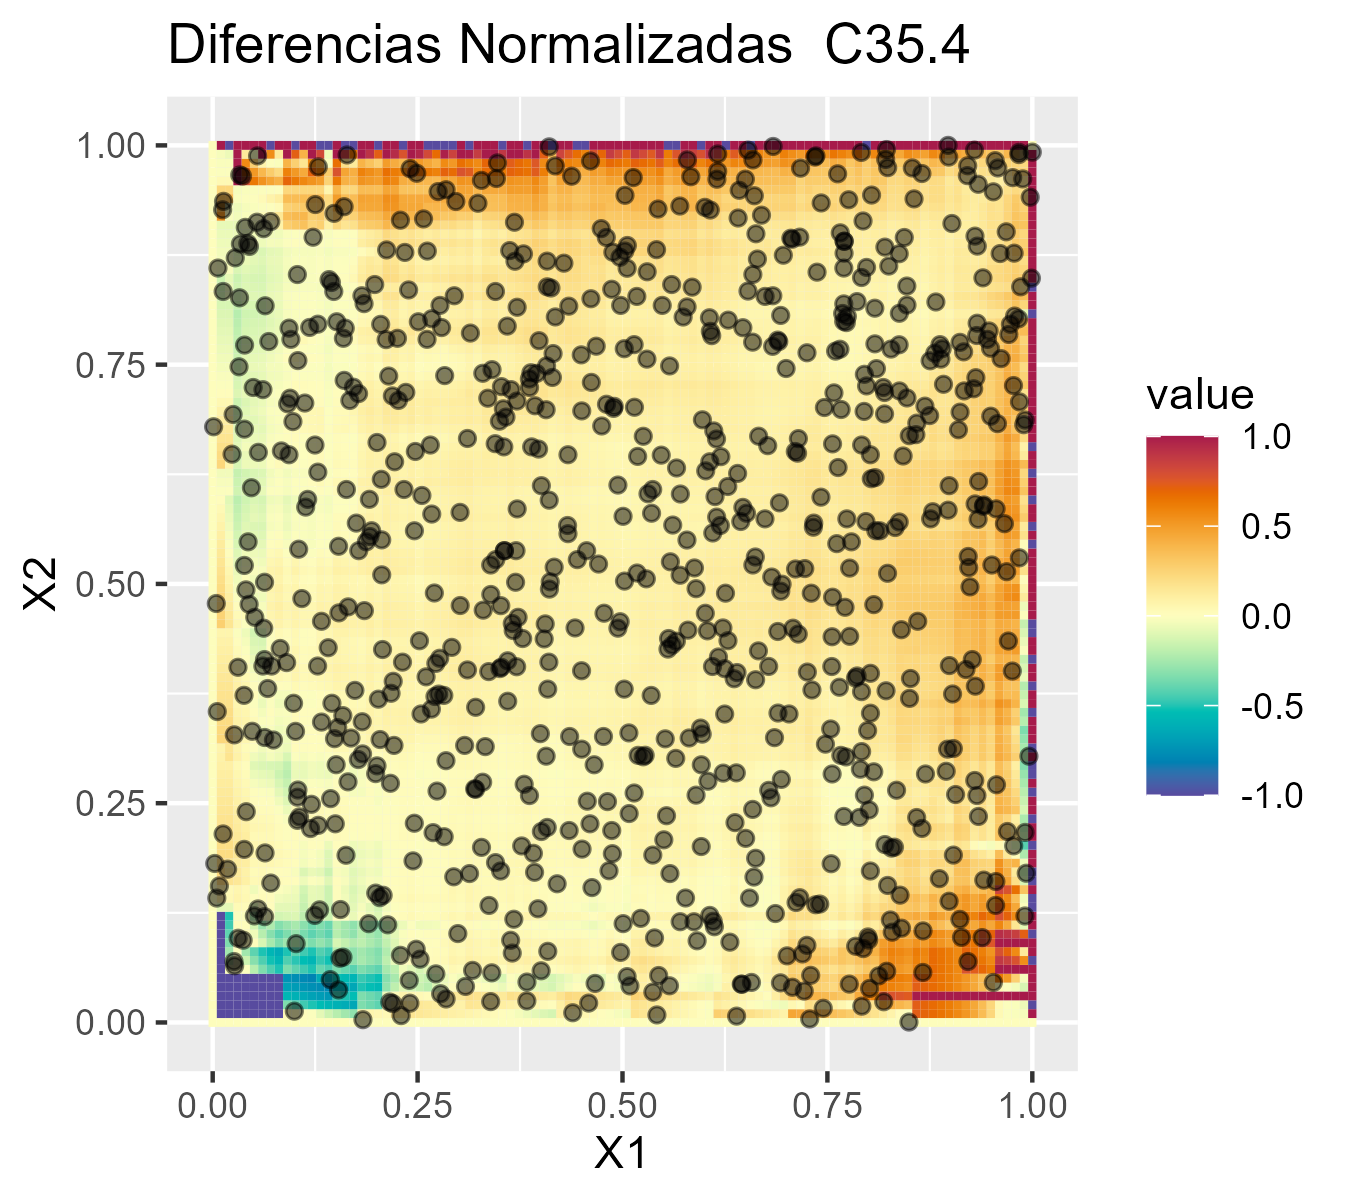
\includegraphics[width=0.33\textwidth]{4img/MujHC35.4.png}}
    \caption{Cópulas ajustadas para mujeres, nivel $2$.}
    \label{fig:Modelo4MujNivel2}
\end{figure}

%%%%%%%%%%%%%%%%%%%%%%%%%%%%%%%%%%%%%%%%%%%%%%%%%%

\begin{figure}[H]
 \centering
  \subfloat[$\mathscr{H}\rho_{C_{14|23}}$]{
   \label{C14.23rho}
    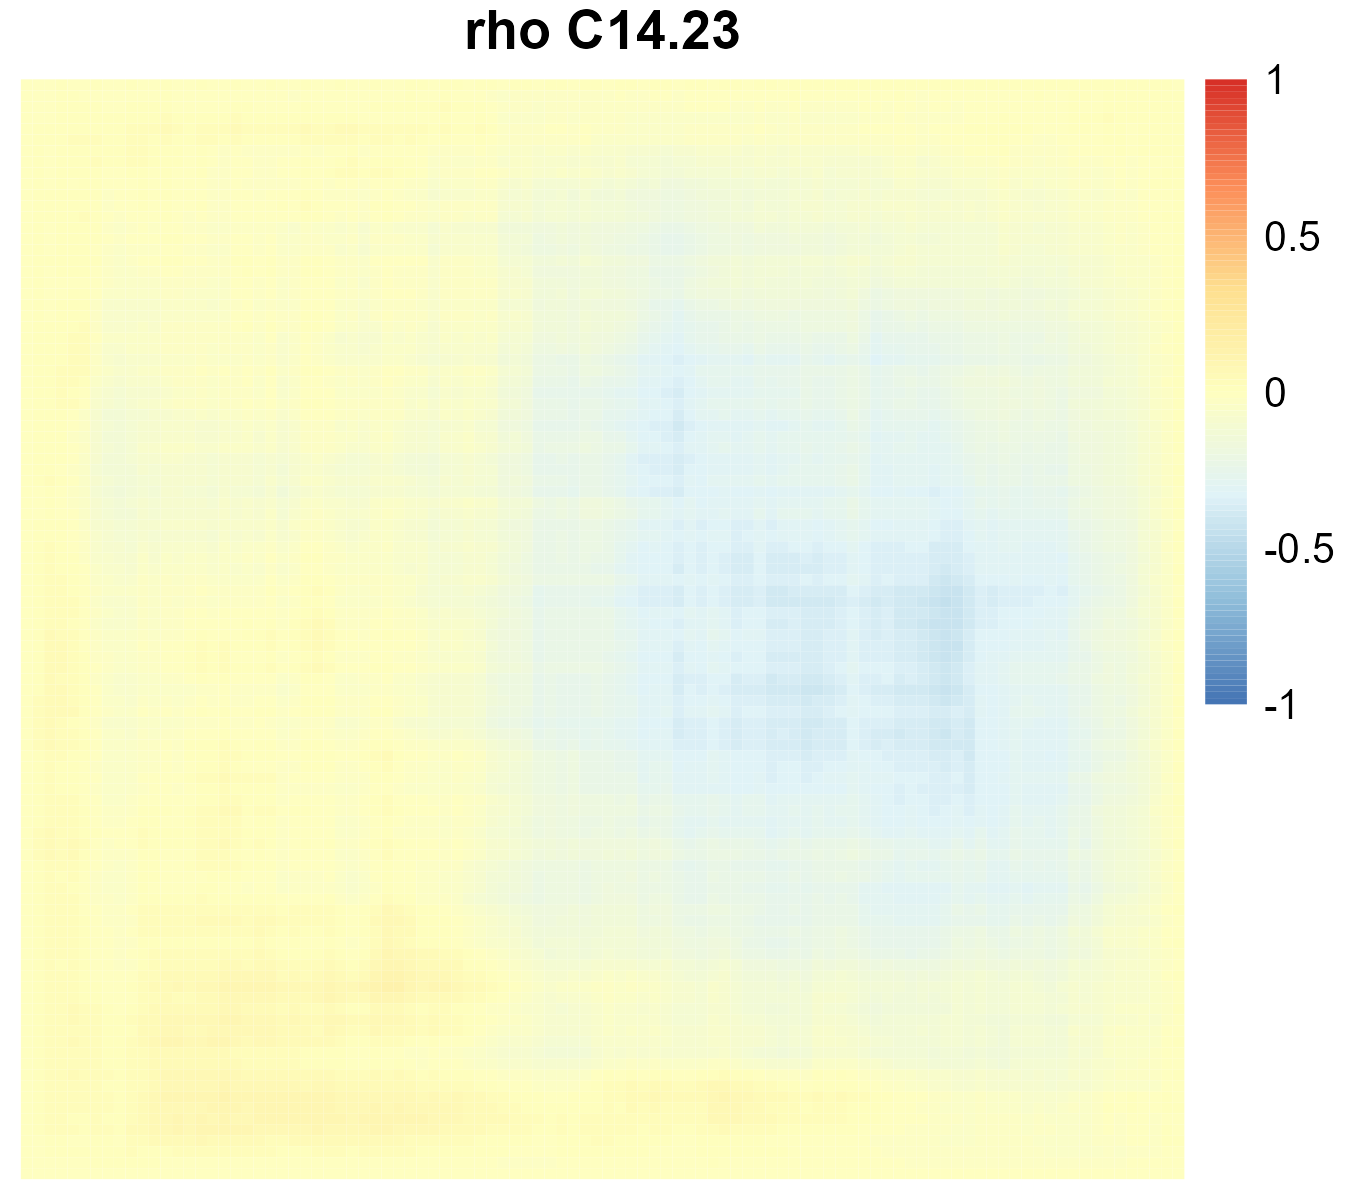
\includegraphics[width=0.3\textwidth]{4img/MujrhoC14.23.png}}
  \subfloat[$\mathscr{H}\sigma_{C_{14|23}}$]{
   \label{C14.23sigma}
    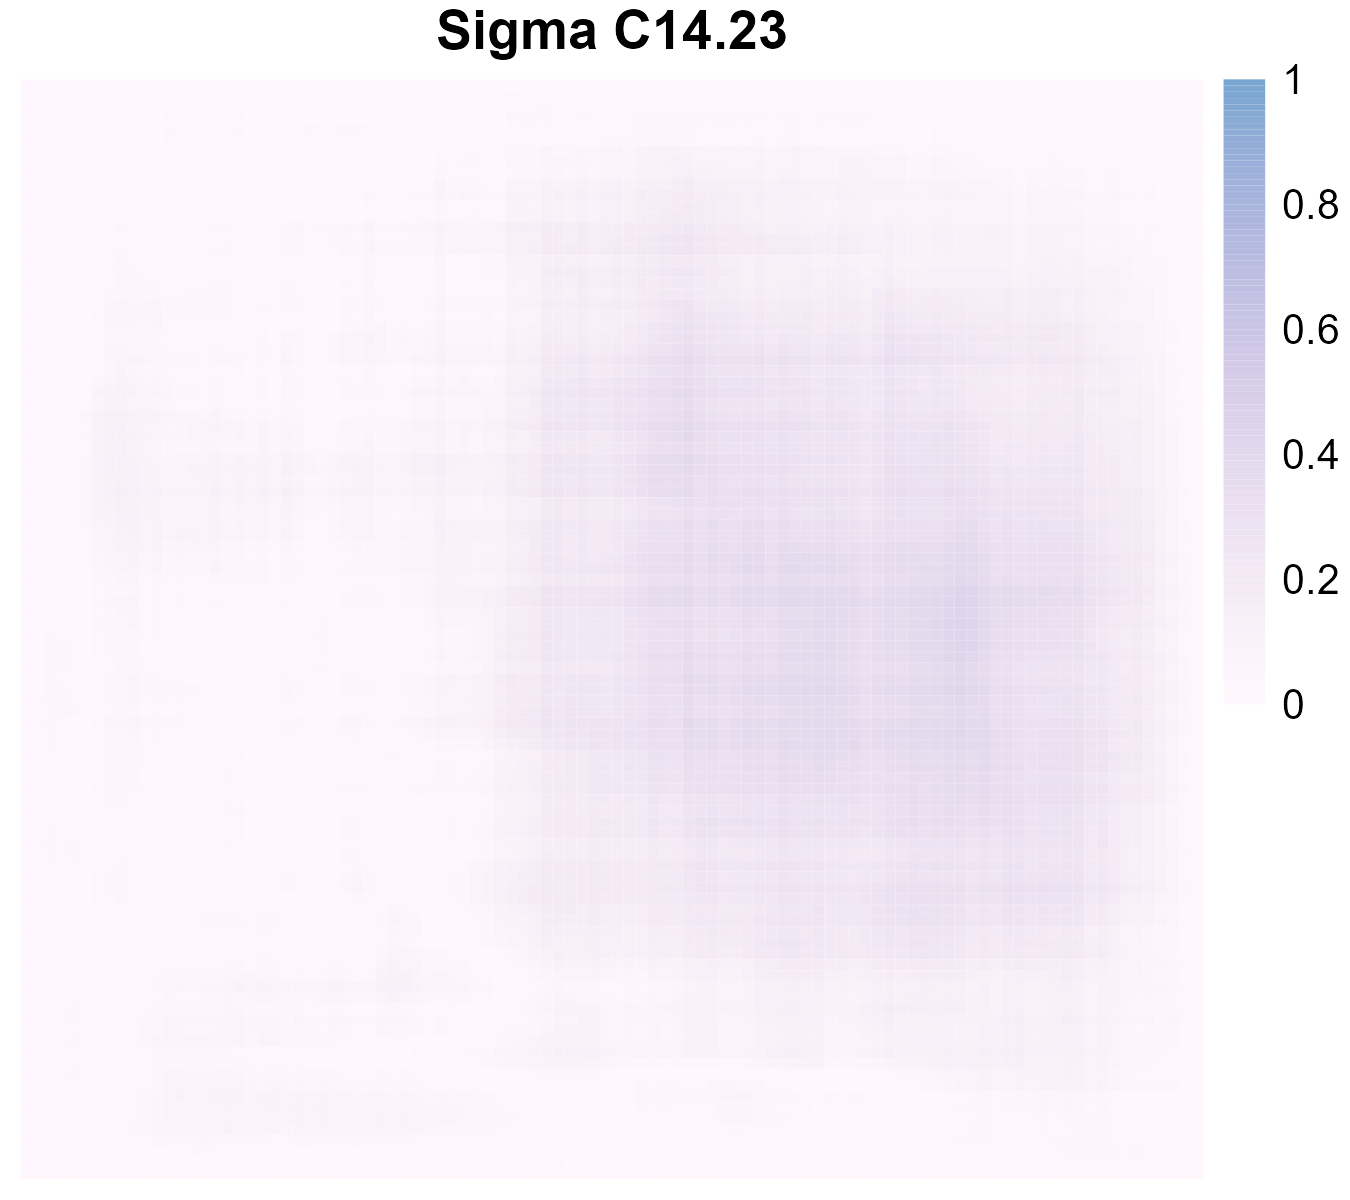
\includegraphics[width=0.3\textwidth]{4img/MujsigmaC14.23.png}}
  \subfloat[$\mathscr{H}_{C_{14|23}}$]{
   \label{C14.23H}
    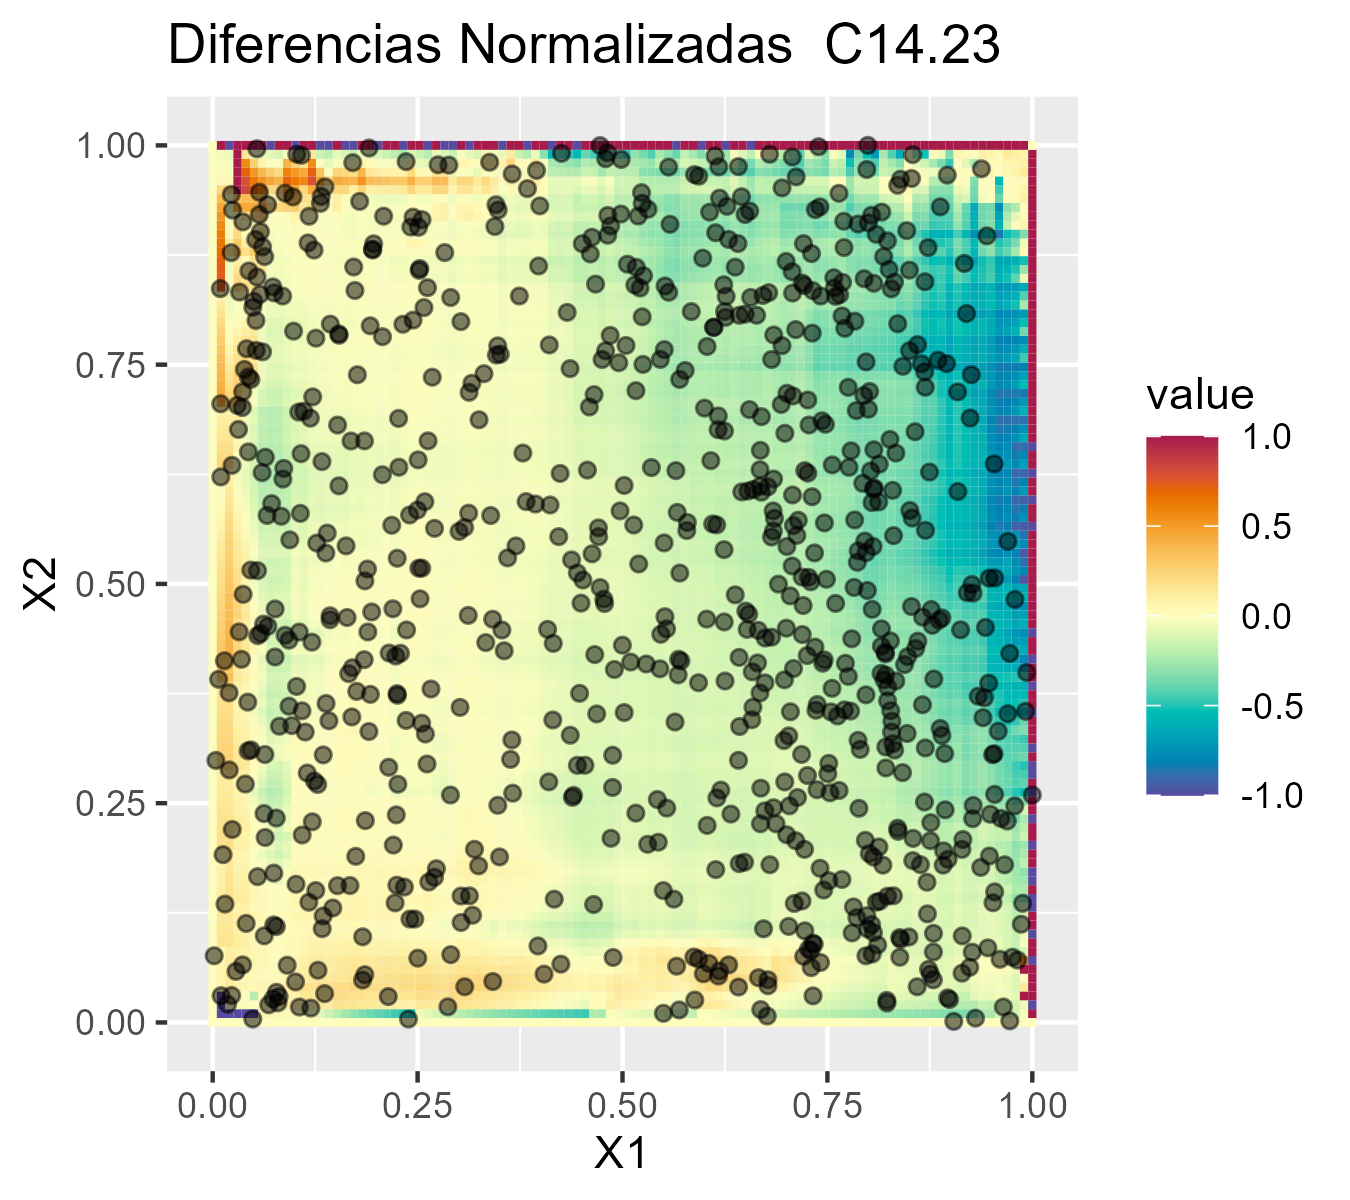
\includegraphics[width=0.3\textwidth]{4img/MujHC14.23.png}}
\end{figure}

\begin{figure}[H]
 \centering
  \subfloat[$\mathscr{H}\rho_{C_{25|34}}$]{
   \label{C25.34rho}
    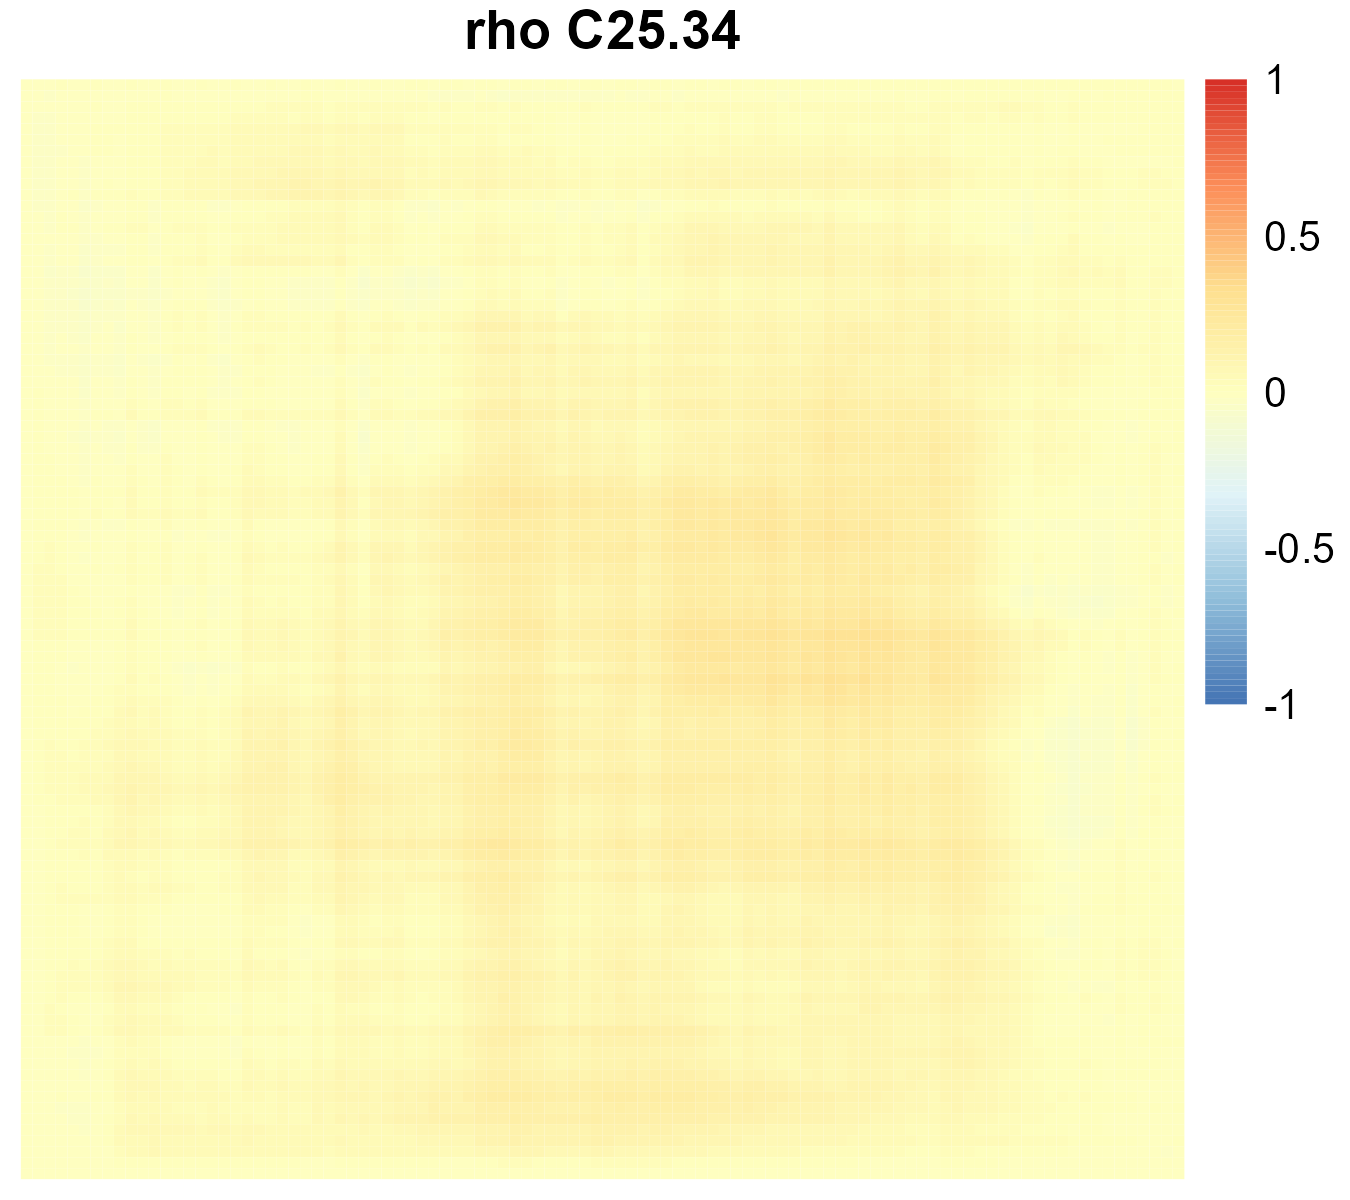
\includegraphics[width=0.3\textwidth]{4img/MujrhoC25.34.png}}
  \subfloat[$\mathscr{H}\sigma_{C_{25|34}}$]{
   \label{C25.34sigma}
    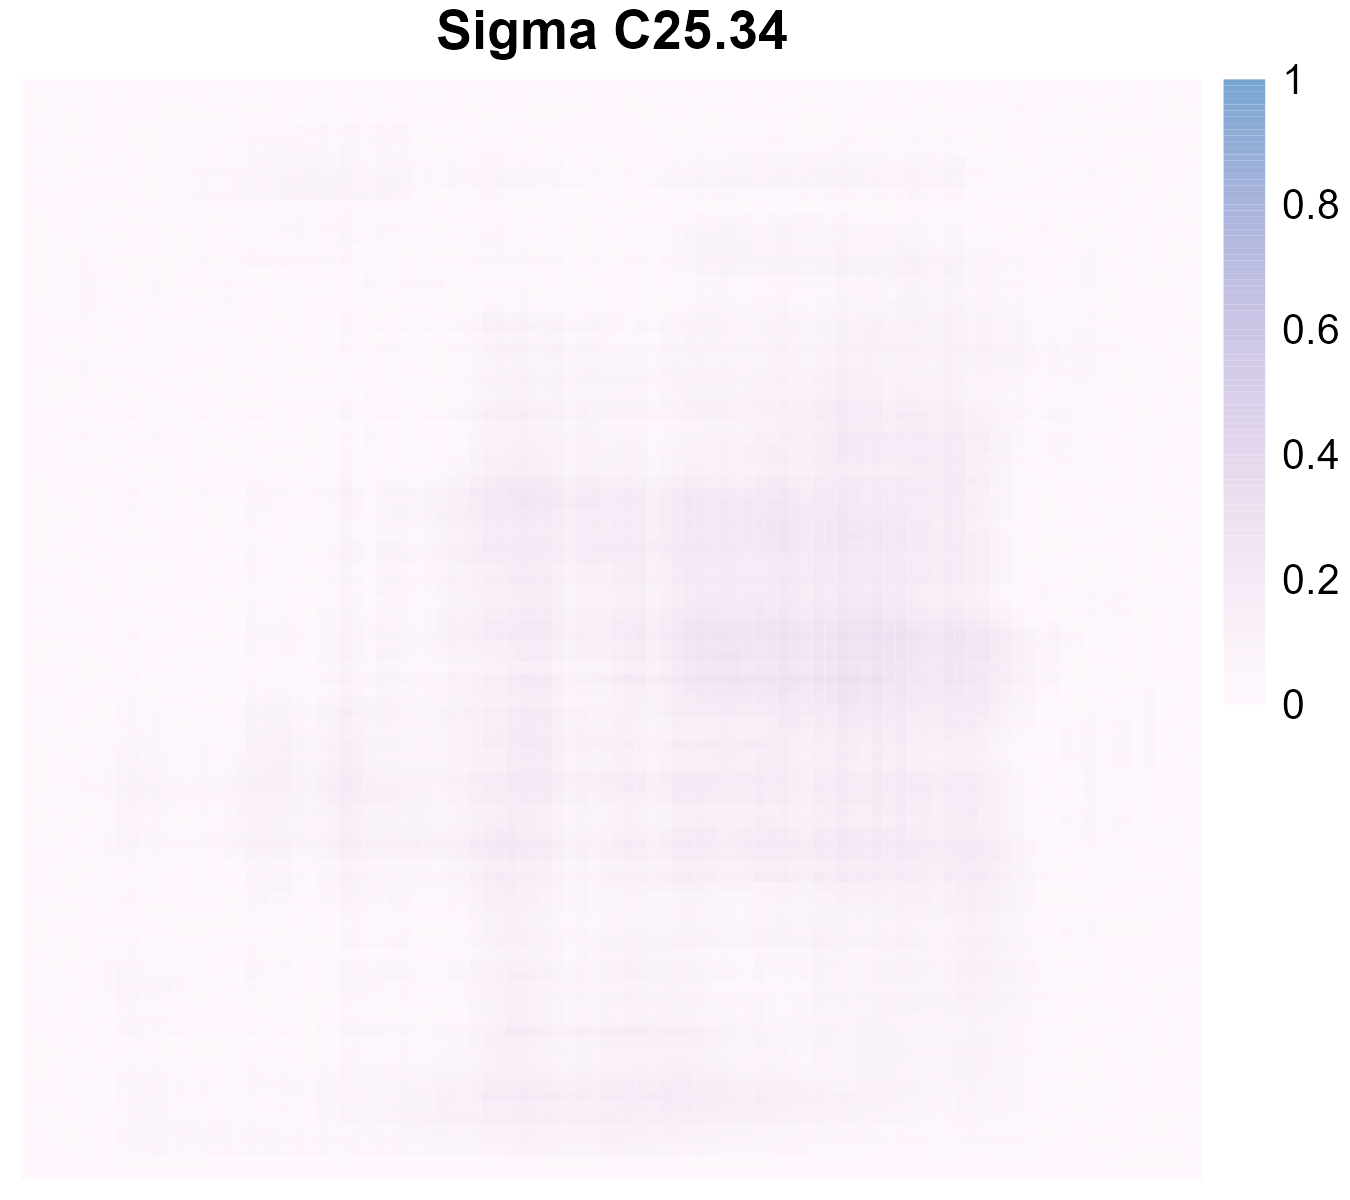
\includegraphics[width=0.3\textwidth]{4img/MujsigmaC25.34.png}}
  \subfloat[$\mathscr{H}_{C_{25|34}}$]{
   \label{C25.34H}
    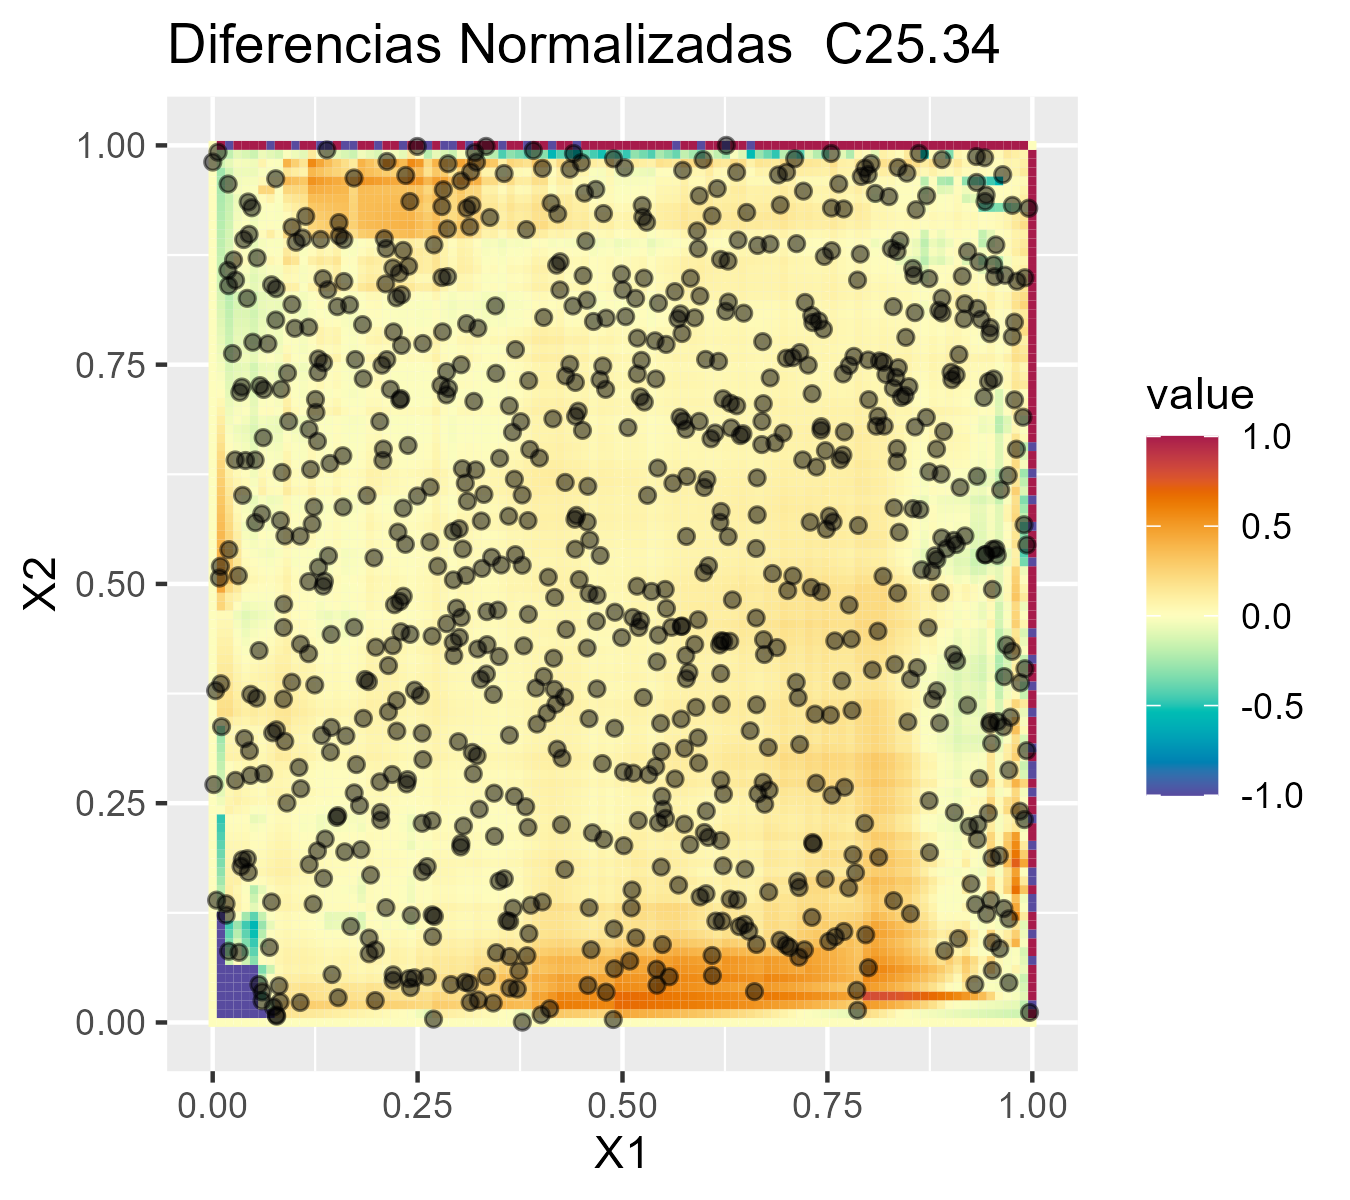
\includegraphics[width=0.3\textwidth]{4img/MujHC25.34.png}}
    \caption{Cópulas ajustadas para Mujeres, nivel $3$.}
    \label{fig:Modelo4MujNivel3}
\end{figure}

%%%%%%%%%%%%%%%%%%%%%%%%%%%%%%%%%%%%%%%%%%%%%%%%%%

\begin{figure}[H]
 \centering
  \subfloat[$\mathscr{H}\rho_{C_{15|234}}$]{
   \label{C15.234rho}
    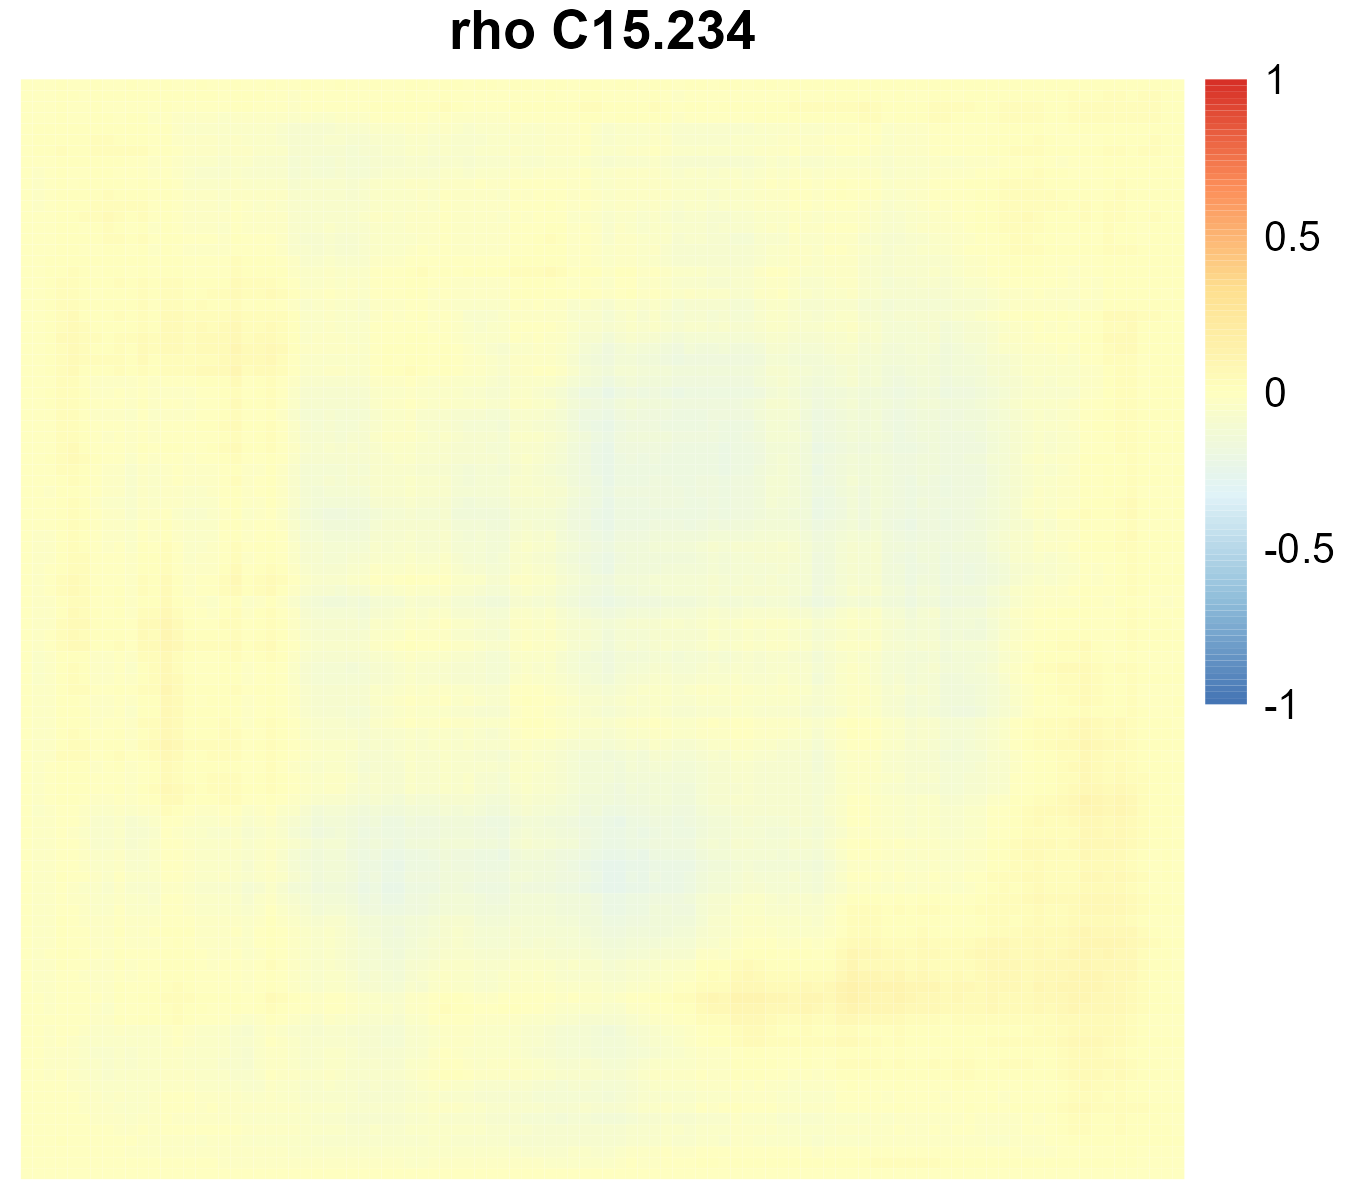
\includegraphics[width=0.3\textwidth]{4img/MujrhoC15.234.png}}
  \subfloat[$\mathscr{H}\sigma_{C_{15|234}}$]{
   \label{C15.234sigma}
    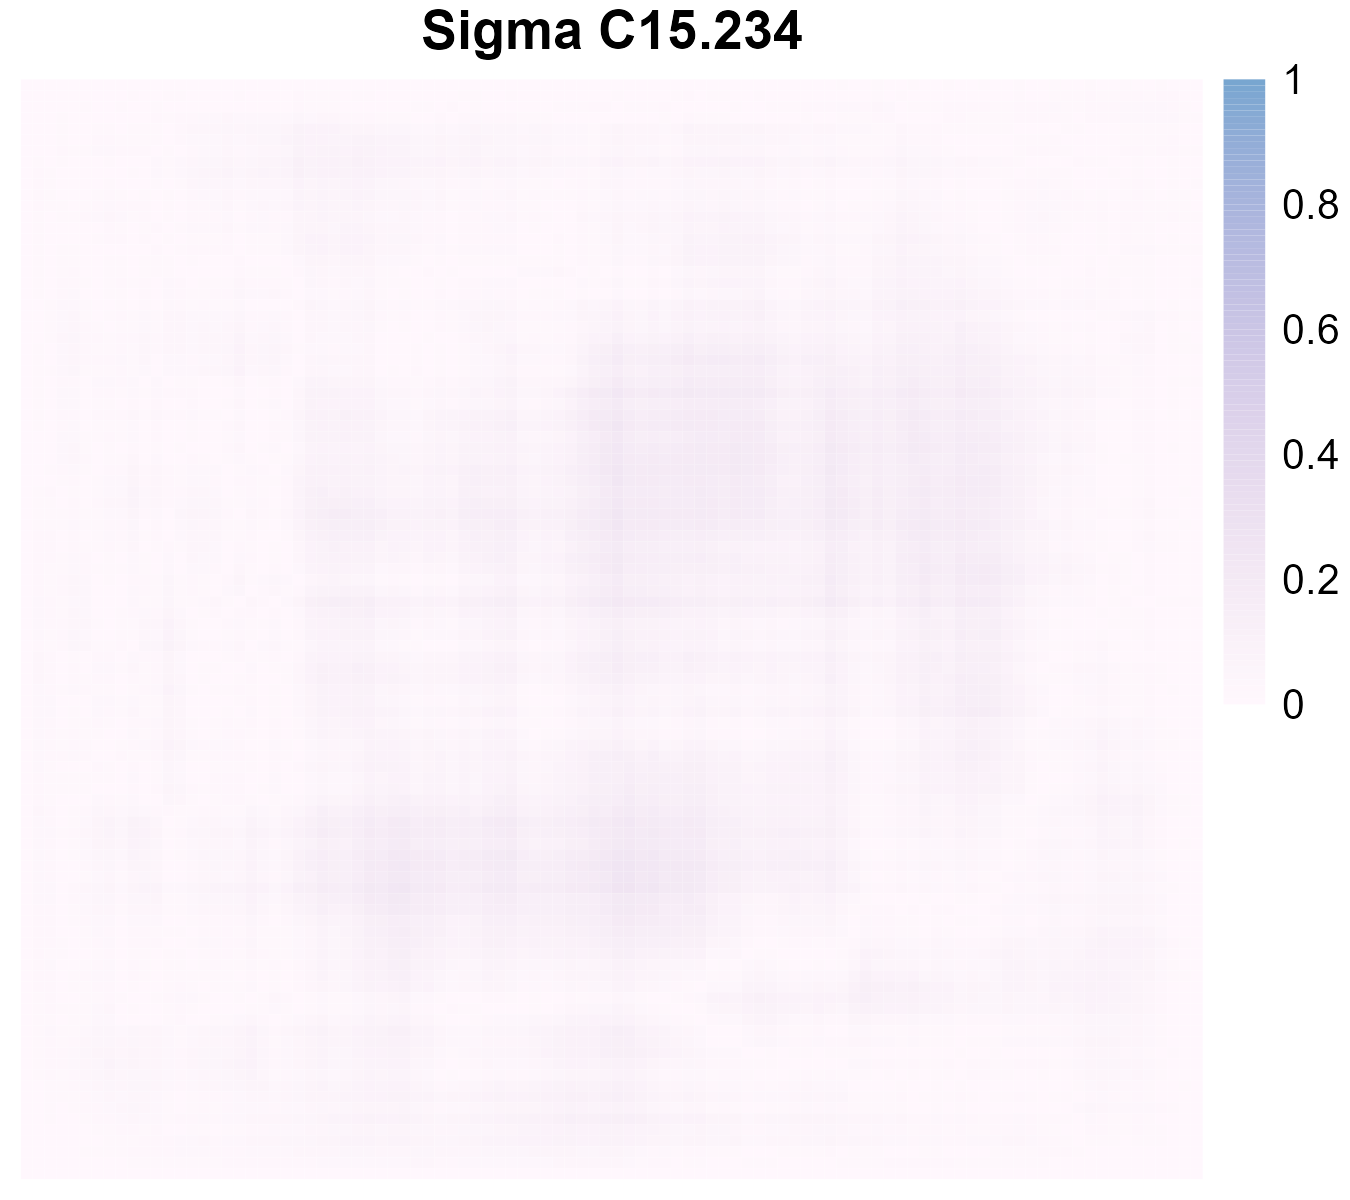
\includegraphics[width=0.3\textwidth]{4img/MujsigmaC15.234.png}}
  \subfloat[$\mathscr{H}_{C_{15|234}}$]{
   \label{C15.234H}
    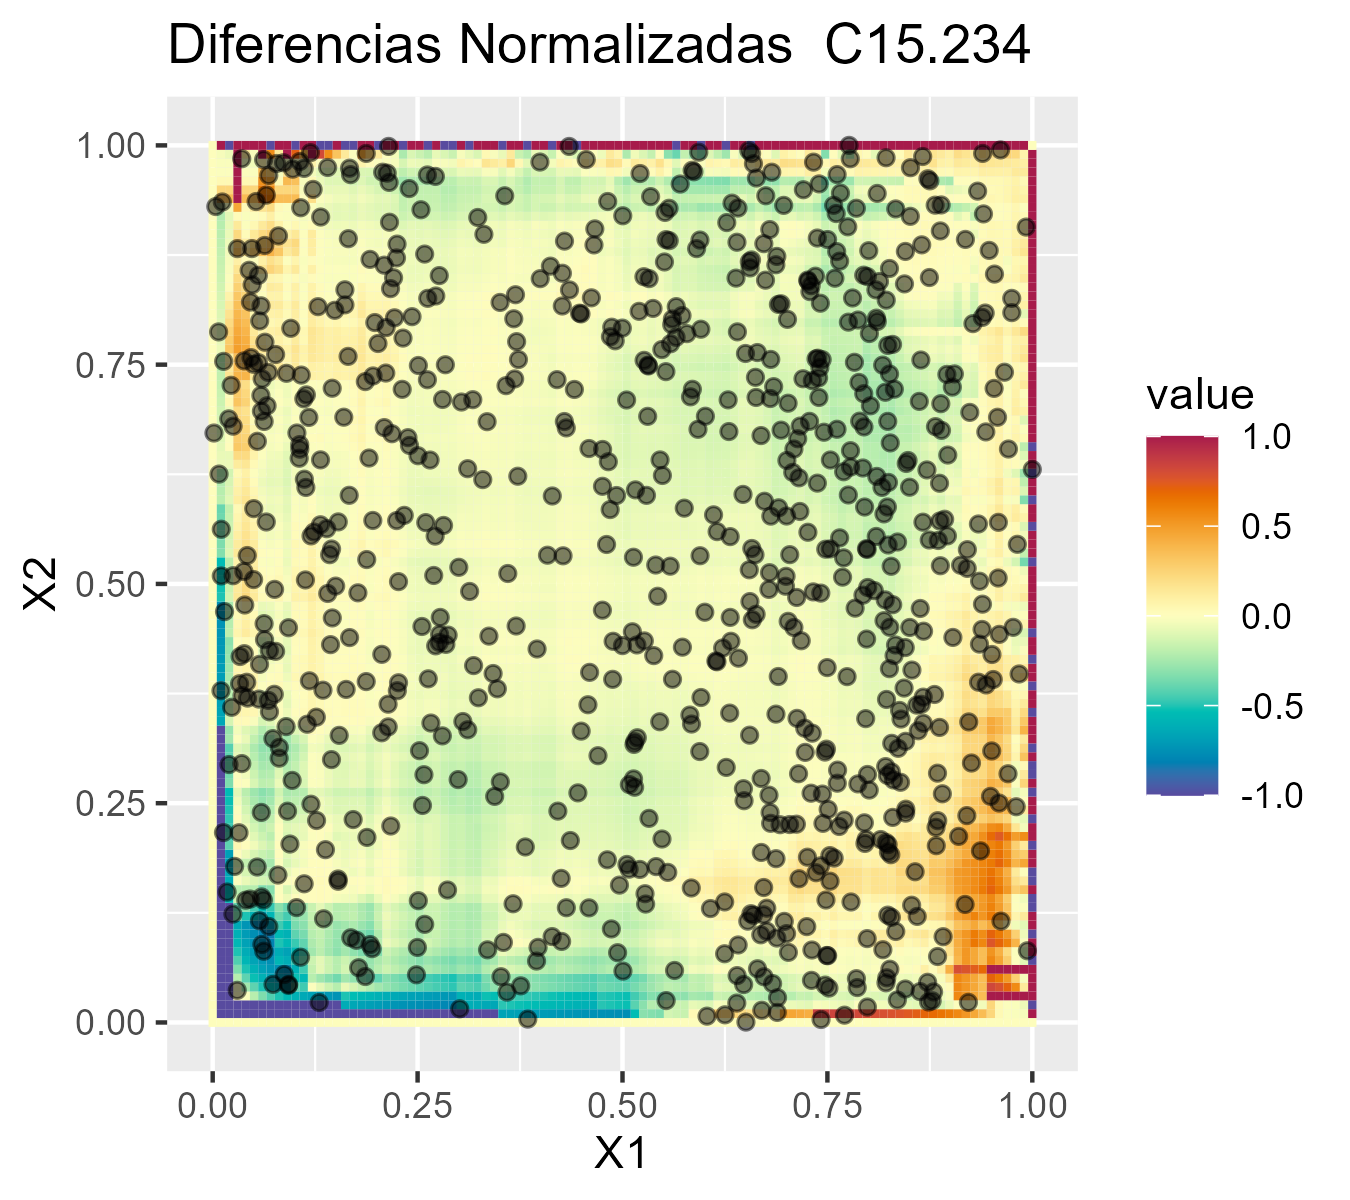
\includegraphics[width=0.3\textwidth]{4img/MujHC15.234.png}}
    \caption{Cópulas ajustadas para mujeres, nivel $3$.}
    \label{fig:Modelo4MujNivel4}
\end{figure}


En las Figuras \ref{fig:Modelo4MujNivel1}, \ref{fig:Modelo4MujNivel2}, \ref{fig:Modelo4MujNivel3} y \ref{fig:Modelo4MujNivel4}, se muestran los heatmaps para cada cópula de modelo de las mujeres, de los nivel $1$, $2$, $3$ y $4$, respectivamente. Las dependencias observadas en las cópulas ajustadas son muy similares a las descritas en las Figuras \ref{fig:Modelo4TotalNivel1}-\ref{fig:Modelo4TotalNivel4} del Capítulo \ref{Resultados}. Sin embargo, para realizar una comparación más detallada, se construyeron los Cuadros \ref{TablaNivel1}, \ref{TablaNivel2}, \ref{TablaNivel3} y \ref{TablaNivel4}, que comparan las cópulas ajustadas en función del conjunto de datos utilizado, estas se ecuentran al final de este apéndice. Estas tablas permiten identificar y analizar las diferencias y similitudes en las estructuras de dependencia entre las diferentes muestras, proporcionando una visión más precisa y matizada de cómo varían las interacciones entre las variables según el dataset empleado.

%%%%%%%%%%%%%%%%%%%%%%%%%%%%%%%%%%%%%%%%%%%%%%%%%%
%%%%%%%%%%%%%%%%%%%%%%%%%%%%%%%%%%%%%%%%%%%%%%%%%%
\begin{figure}[H]
    \centering
    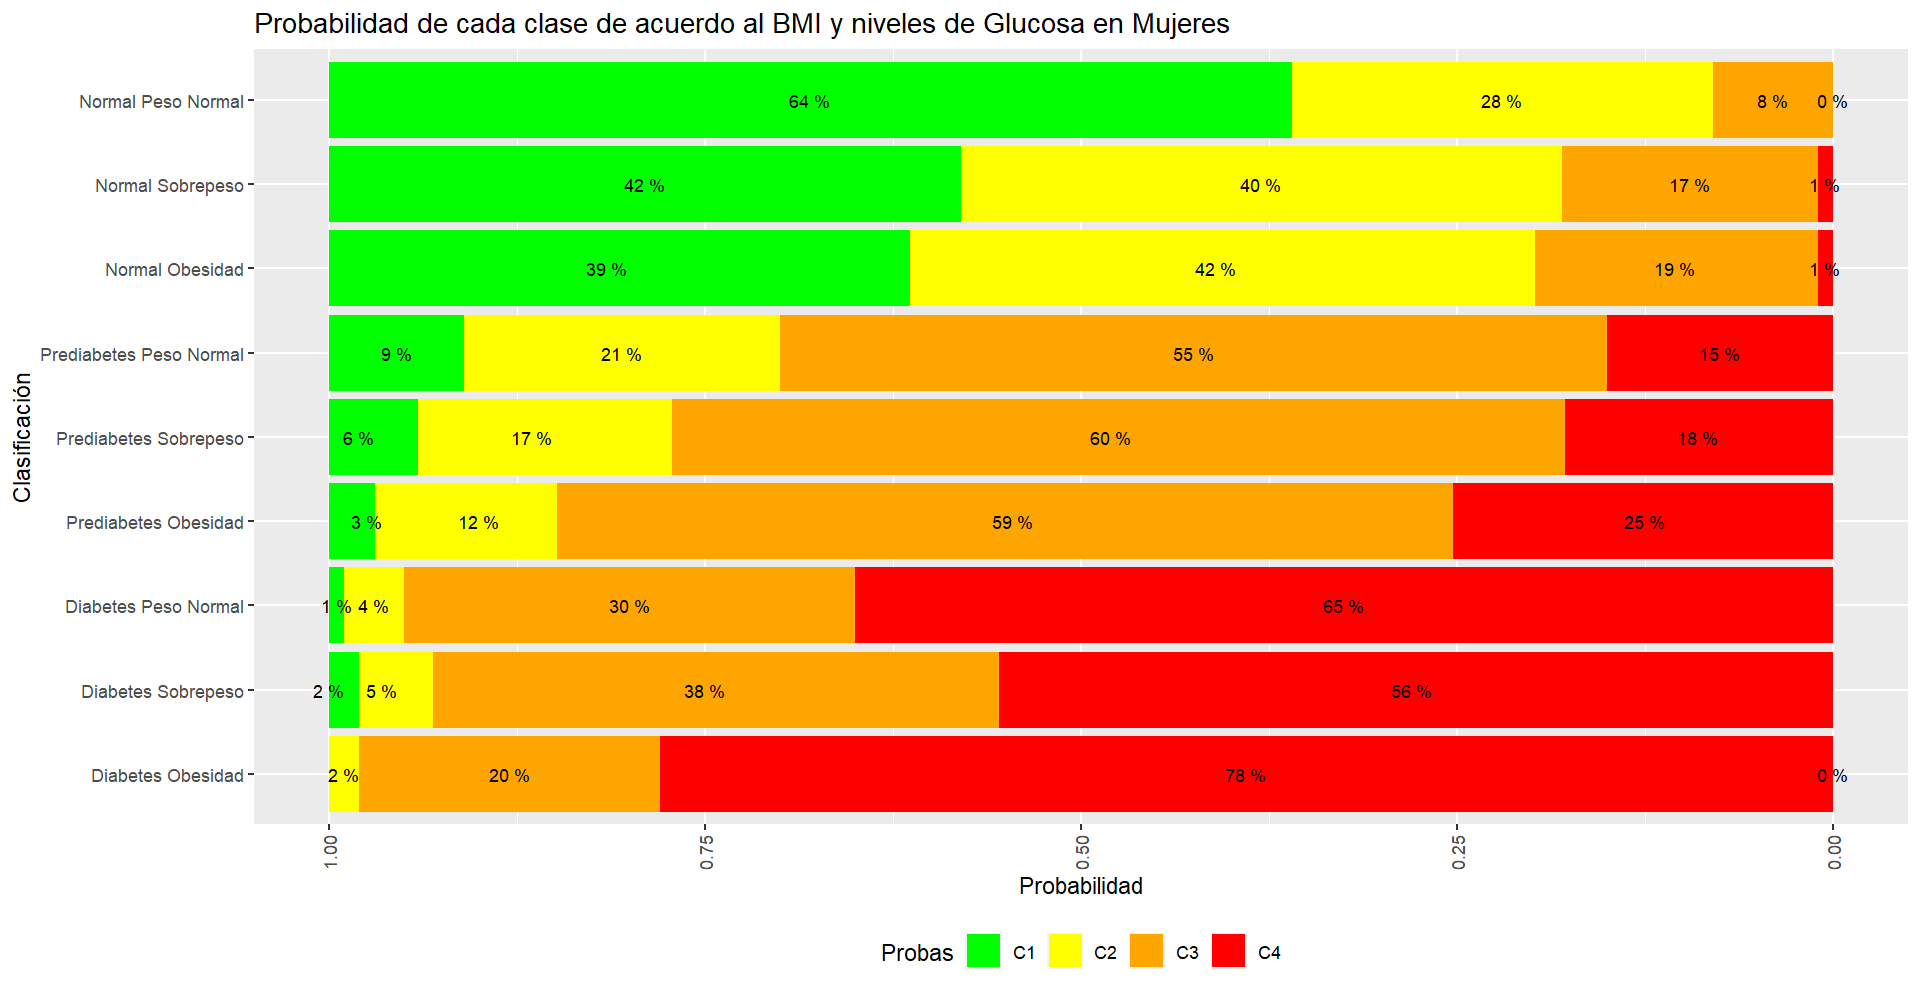
\includegraphics[height = 10 cm, width = 0.9 \textwidth]{4img/tablaM.png}
    \caption{Tabla de probabilidades de cada clase de mujeres.}
    \label{fig:tabMujeres}
\end{figure}

En la Figura \ref{fig:tabMujeres}, se observa que la probabilidad de pertenecer a la clase de individuos saludables es muy alta para las personas con niveles de glucosa normales y un peso normal. Sin embargo, en la categoría de personas con niveles de glucosa normales pero con obesidad o sobrepeso, la probabilidad de desarrollar resistencia a la insulina con predisfunción de las células beta aumenta significativamente, y estos cambios son más bruscos que los observados en la Figura \ref{fig:tabla4varTotal}. A partir de esta categoría, la probabilidad de tener resistencia a la insulina con estrés en las células beta aumenta, predominando en todas las clasificaciones con niveles de glucosa prediabéticos. Las categorías cuyos niveles de glucosa son diabéticos ya se clasifican como pacientes con resistencia a la insulina con disfunción de las células beta. En comparación con la Figura  \ref{fig:tabla4varTotal}, la diferencia más destacable es que los cambios en las probabilidades de las clases son más abruptos. 


%%%%%%%%%%%%%%%%%%%%%%%%%%%%%%%%%%%%%%%%%%%%%%%%%%
%%%%%%%%%%%%%%%%%%%%%%%%%%%%%%%%%%%%%%%%%%%%%%%%%%
%%%%%%%%%%%%%%%%%%%%%%%%%%%%%%%%%%%%%%%%%%%%%%%%%%
%%%%%%%%%%%%%%%%%%%%%%%%%%%%%%%%%%%%%%%%%%%%%%%%%%

\begin{landscape}
\subsection{Visualización del Modelo para Hombres}

\begin{figure}[H]
    \centering
    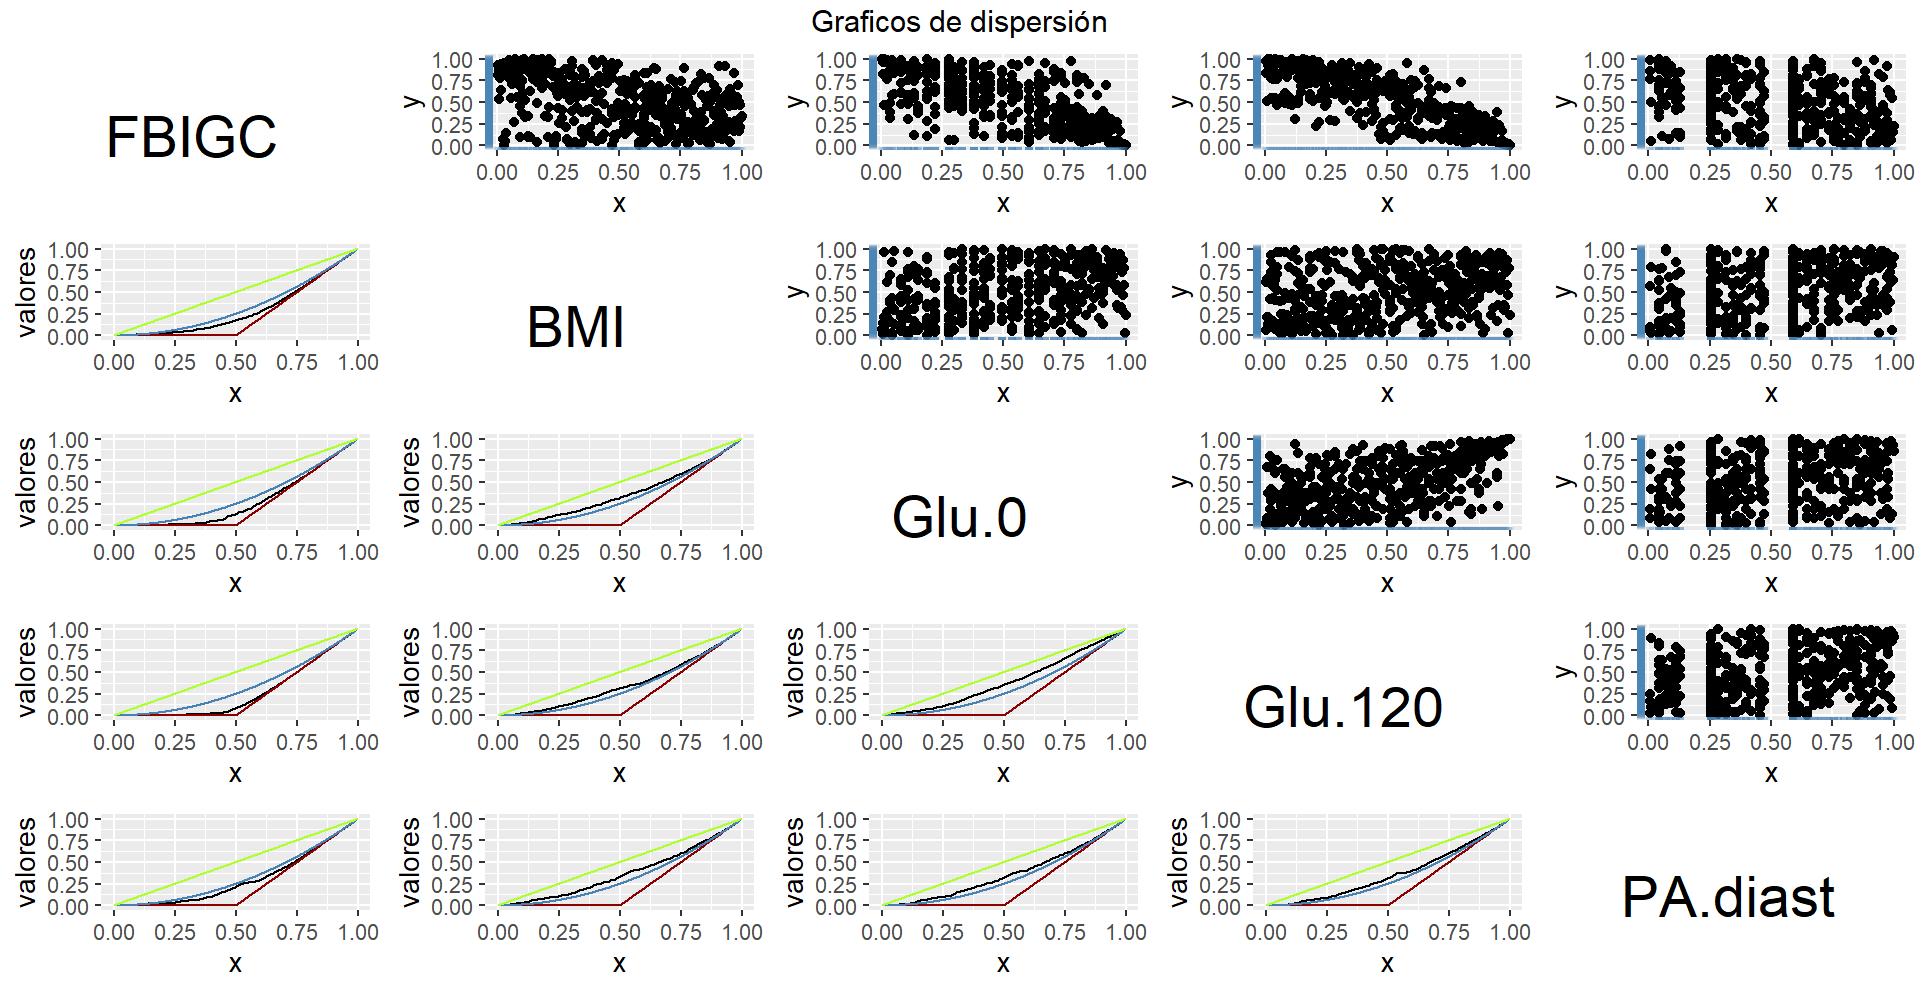
\includegraphics[height = 13.5 cm, width = 1.4 \textwidth]{4img/UdiagH.png}
    \caption{Diagonales y gráficos de dispersión en escala $u$.}
    \label{fig:diagHo}
\end{figure}
\end{landscape}

En la Figura \ref{fig:diagHo}, se presentan las diagonales de las cópulas empíricas con respecto a las diagonales de cópulas de referencia, junto con los gráficos de dispersión de las variables de individuos del género masculino. Al igual que en el caso de hombres y mujeres y solo mujeres, en su mayor parte, la diagonal de la cópula empírica se encuentra por debajo o por encima de la diagonal, lo que indica que las dependencias entre las variables son mayoritariamente concordantes negativas o positivas, respectivamente. También se observa la misma partición generada por la variable de presión diastólica.

\begin{figure}[H]
 \centering
  \subfloat[$\mathscr{H}\rho_{C_{12}}$]{
   \label{C12rhoH}
    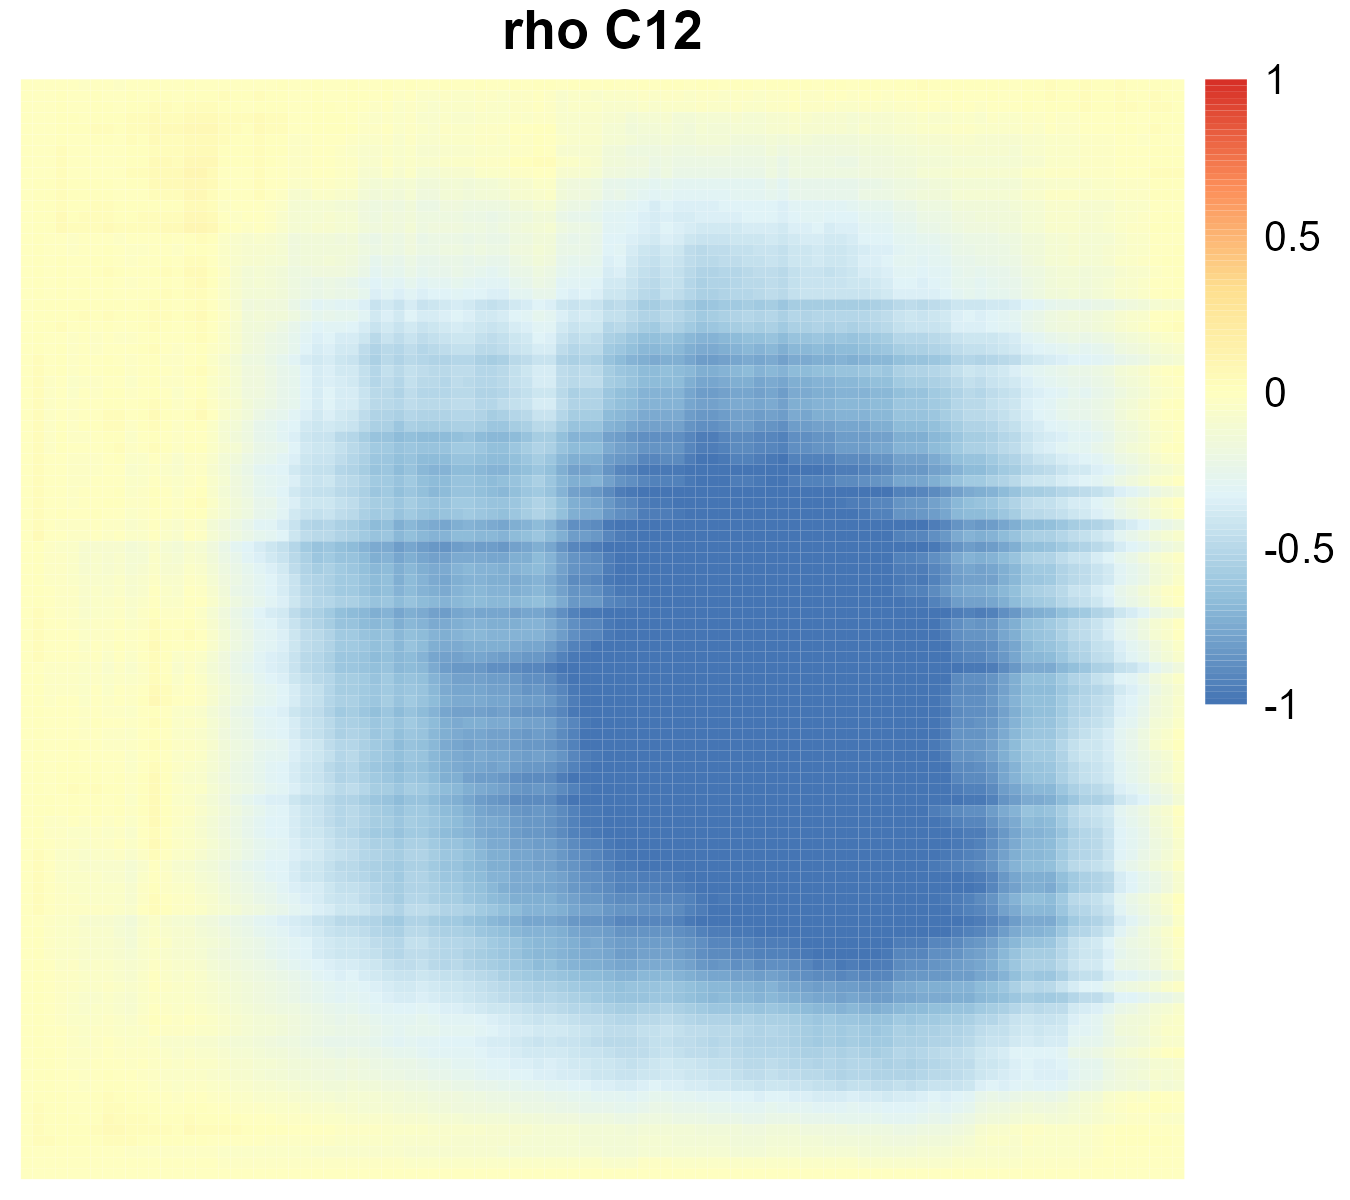
\includegraphics[width=0.3\textwidth]{4img/HomrhoC12.png}}
  \subfloat[$\mathscr{H}\sigma_{C_{12}}$]{
   \label{C12sigmaH}
    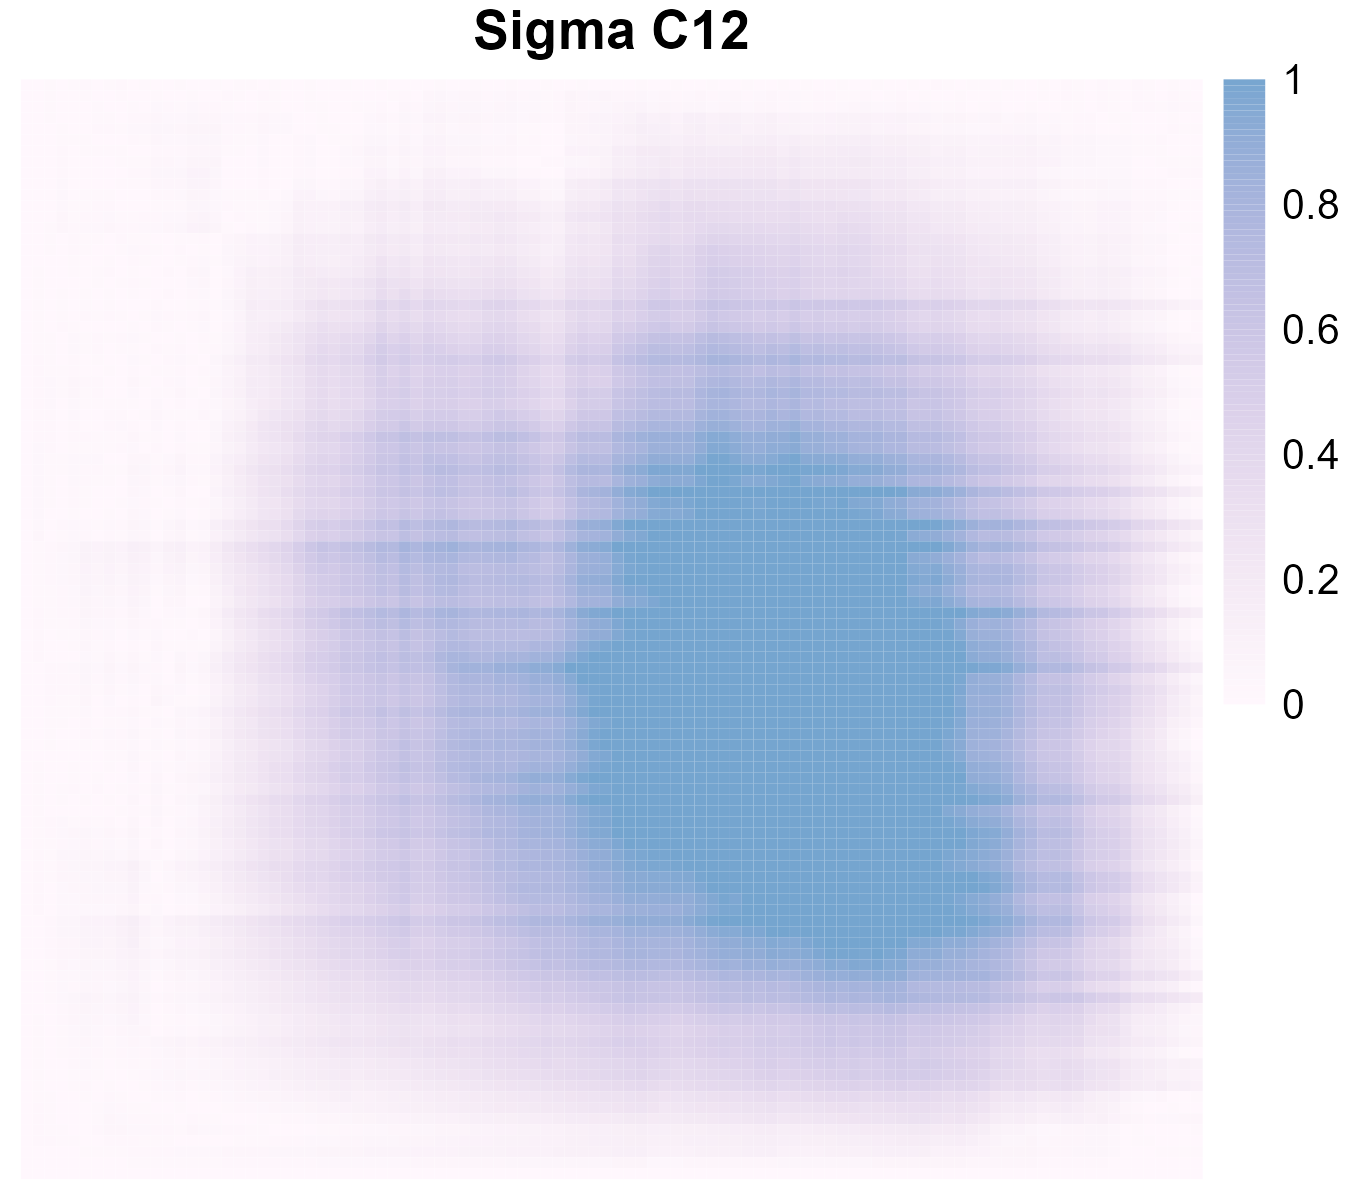
\includegraphics[width=0.3\textwidth]{4img/HomsigmaC12.png}}
  \subfloat[$\mathscr{H}_{C_{12}}$]{
   \label{C12HH}
    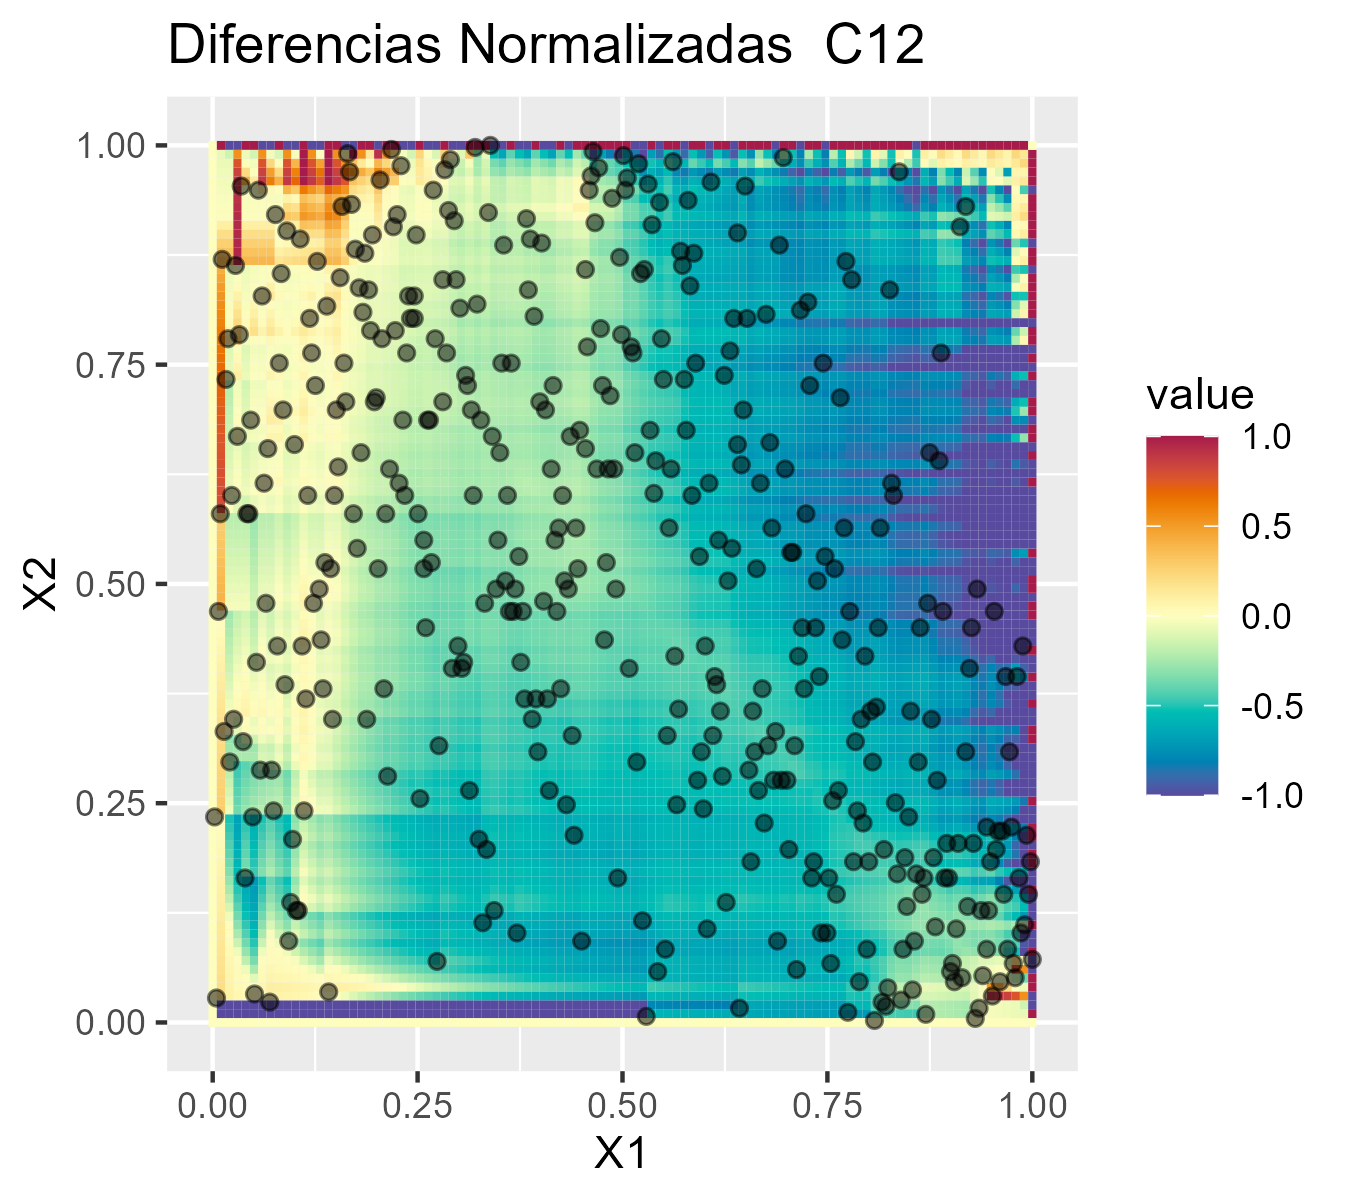
\includegraphics[width=0.3\textwidth]{4img/HomHC12.png}}
\end{figure}

\begin{figure}[H]
 \centering
  \subfloat[$\mathscr{H}\rho_{C_{23}}$]{
   \label{C23rhoH}
    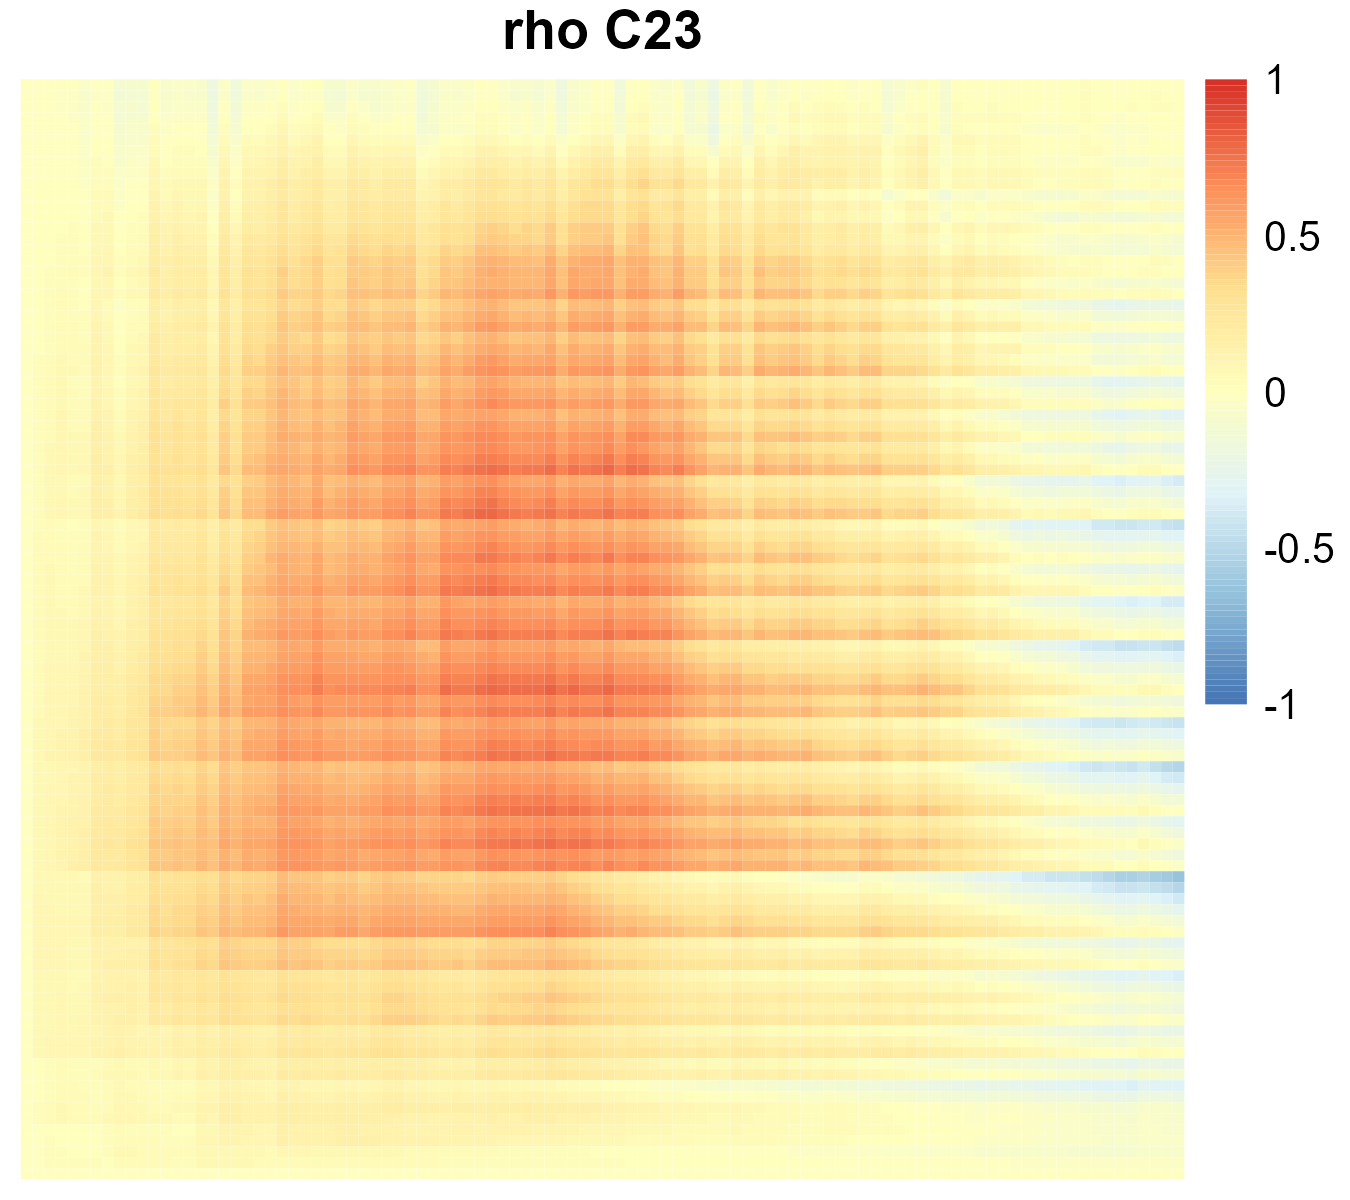
\includegraphics[width=0.3\textwidth]{4img/HomrhoC23.png}}
  \subfloat[$\mathscr{H}\sigma_{C_{23}}$]{
   \label{C23sigmaH}
    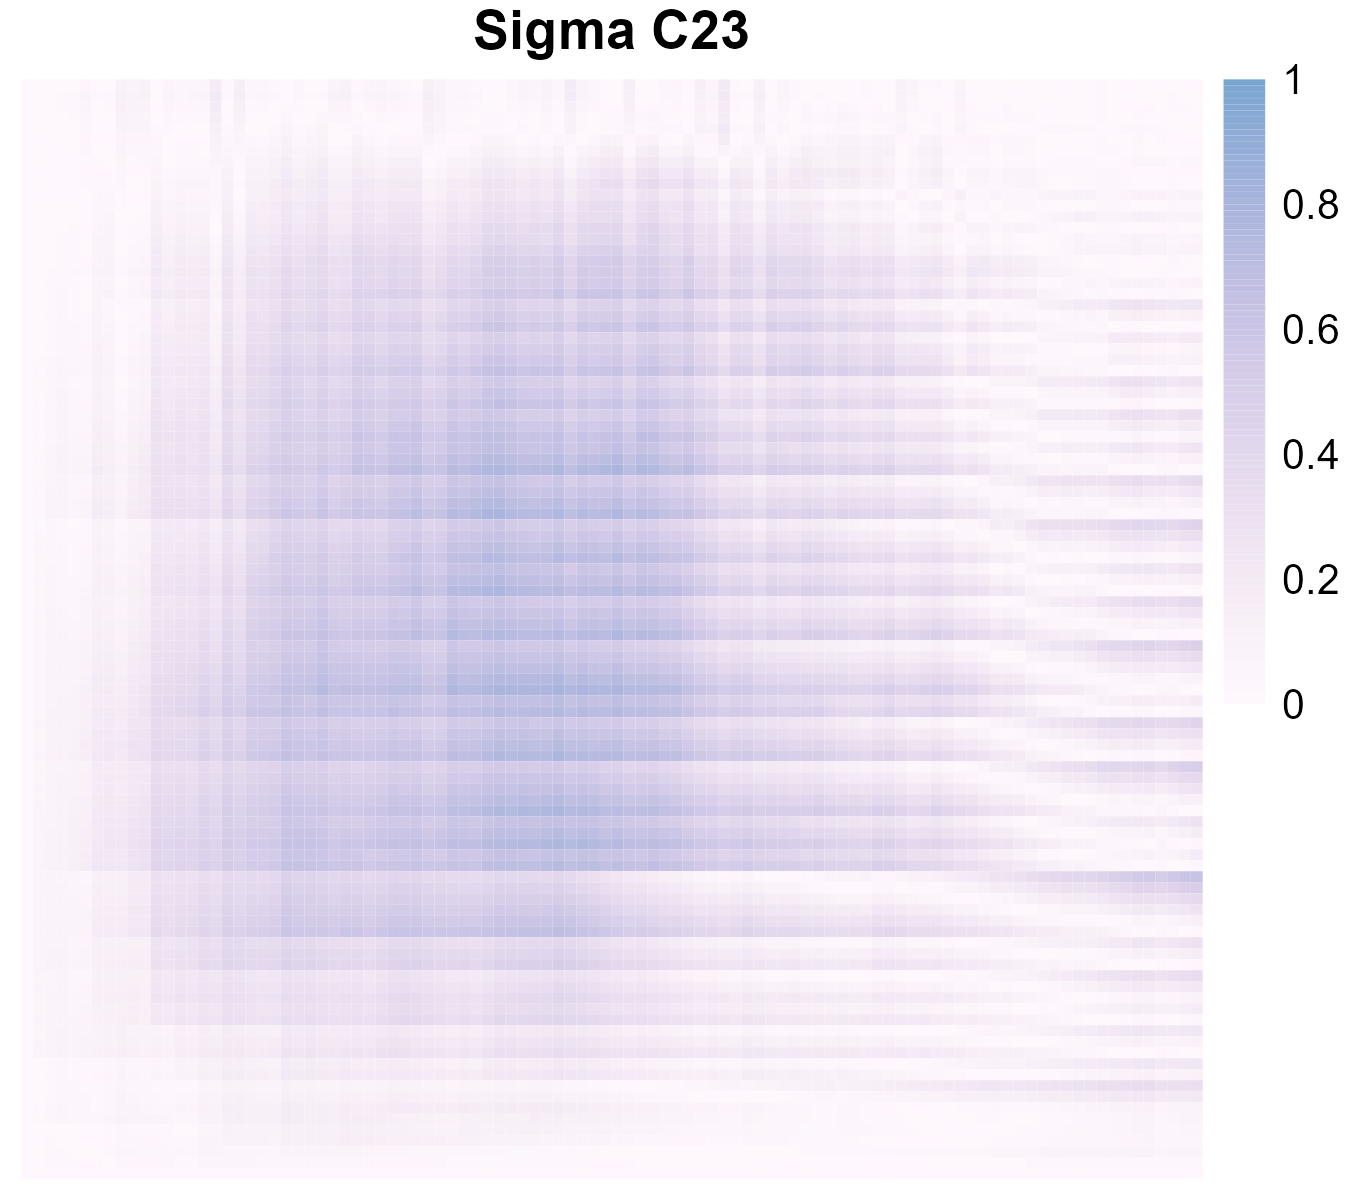
\includegraphics[width=0.3\textwidth]{4img/HomsigmaC23.png}}
  \subfloat[$\mathscr{H}_{C_{23}}$]{
   \label{C23HH}
    \includegraphics[width=0.3\textwidth]{4img/HomHC23.png}}
\end{figure}

\begin{figure}[H]
 \centering
  \subfloat[$\mathscr{H}\rho_{C_{34}}$]{
   \label{C34rhoH}
    \includegraphics[width=0.3\textwidth]{4img/HomrhoC34.png}}
  \subfloat[$\mathscr{H}\sigma_{C_{34}}$]{
   \label{C34sigmaH}
    \includegraphics[width=0.3\textwidth]{4img/HomsigmaC34.png}}
  \subfloat[$\mathscr{H}_{C_{34}}$]{
   \label{C34HH}
    \includegraphics[width=0.3\textwidth]{4img/HomHC34.png}}
\end{figure}

\begin{figure}[H]
 \centering
  \subfloat[$\mathscr{H}\rho_{C_{45}}$]{
   \label{C45rhoH}
    \includegraphics[width=0.3\textwidth]{4img/HomrhoC45.png}}
  \subfloat[$\mathscr{H}\sigma_{C_{45}}$]{
   \label{C45sigmaH}
    \includegraphics[width=0.3\textwidth]{4img/HomsigmaC45.png}}
  \subfloat[$\mathscr{H}_{C_{45}}$]{
   \label{C45HH}
    \includegraphics[width=0.3\textwidth]{4img/HomHC45.png}}
    \caption{Cópulas ajustadas para hombres, nivel $1$.}
    \label{fig:Modelo4HomNivel1}
\end{figure}

%%%%%%%%%%%%%%%%%%%%%%%%%%%%%%%%%%%%%%%%%%%%%%%%


\begin{figure}[H]
 \centering
  \subfloat[$\mathscr{H}\rho_{C_{13|2}}$]{
   \label{C13.2rhoH}
    \includegraphics[width=0.3\textwidth]{4img/HomrhoC13.2.png}}
  \subfloat[$\mathscr{H}\sigma_{C_{13|2}}$]{
   \label{C13.2sigmaH}
    \includegraphics[width=0.3\textwidth]{4img/HomsigmaC13.2.png}}
  \subfloat[$\mathscr{H}_{C_{13|2}}$]{
   \label{C13.2HH}
    \includegraphics[width=0.3\textwidth]{4img/HomHC13.2.png}}
\end{figure}

\begin{figure}[H]
 \centering
  \subfloat[$\mathscr{H}\rho_{C_{24|3}}$]{
   \label{C24.3rhoH}
    \includegraphics[width=0.3\textwidth]{4img/HomrhoC24.3.png}}
  \subfloat[$\mathscr{H}\sigma_{C_{24|3}}$]{
   \label{C24.3sigmaH}
    \includegraphics[width=0.3\textwidth]{4img/HomsigmaC24.3.png}}
  \subfloat[$\mathscr{H}_{C_{24|3}}$]{
   \label{C24.3HH}
    \includegraphics[width=0.3\textwidth]{4img/HomHC24.3.png}}
\end{figure}

\begin{figure}[H]
 \centering
  \subfloat[$\mathscr{H}\rho_{C_{35|4}}$]{
   \label{C35.4rhoH}
    \includegraphics[width=0.3\textwidth]{4img/HomrhoC35.4.png}}
  \subfloat[$\mathscr{H}\sigma_{C_{35|4}}$]{
   \label{C35.4sigmaH}
    \includegraphics[width=0.3\textwidth]{4img/HomsigmaC35.4.png}}
  \subfloat[$\mathscr{H}_{C_{35|4}}$]{
   \label{C35.4HH}
    \includegraphics[width=0.3\textwidth]{4img/HomHC35.4.png}}
    \caption{Cópulas ajustadas para hombres, nivel $2$.}
    \label{fig:Modelo4HomNivel2}
\end{figure}

%%%%%%%%%%%%%%%%%%%%%%%%%%%%%%%%%%%%%%%%%%%%%%%%%%

\begin{figure}[H]
 \centering
  \subfloat[$\mathscr{H}\rho_{C_{14|23}}$]{
   \label{C14.23rhoH}
    \includegraphics[width=0.3\textwidth]{4img/HomrhoC14.23.png}}
  \subfloat[$\mathscr{H}\sigma_{C_{14|23}}$]{
   \label{C14.23sigmaH}
    \includegraphics[width=0.3\textwidth]{4img/HomsigmaC14.23.png}}
  \subfloat[$\mathscr{H}_{C_{14|23}}$]{
   \label{C14.23HH}
    \includegraphics[width=0.3\textwidth]{4img/HomHC14.23.png}}
\end{figure}

\begin{figure}[H]
 \centering
  \subfloat[$\mathscr{H}\rho_{C_{25|34}}$]{
   \label{C25.34rhoH}
    \includegraphics[width=0.3\textwidth]{4img/HomrhoC25.34.png}}
  \subfloat[$\mathscr{H}\sigma_{C_{25|34}}$]{
   \label{C25.34sigmaH}
    \includegraphics[width=0.3\textwidth]{4img/HomsigmaC25.34.png}}
  \subfloat[$\mathscr{H}_{C_{25|34}}$]{
   \label{C25.34HH}
    \includegraphics[width=0.3\textwidth]{4img/HomHC25.34.png}}
    \caption{Cópulas ajustadas para hombres, nivel $3$.}
    \label{fig:Modelo4HomNivel3}
\end{figure}

%%%%%%%%%%%%%%%%%%%%%%%%%%%%%%%%%%%%%%%%%%%%%%%%%%

\begin{figure}[H]
 \centering
  \subfloat[$\mathscr{H}\rho_{C_{15|234}}$]{
   \label{C15.234rhoH}
    \includegraphics[width=0.3\textwidth]{4img/HomrhoC15.234.png}}
  \subfloat[$\mathscr{H}\sigma_{C_{15|234}}$]{
   \label{C15.234sigmaH}
    \includegraphics[width=0.3\textwidth]{4img/HomsigmaC15.234.png}}
  \subfloat[$\mathscr{H}_{C_{15|234}}$]{
   \label{C15.234HH}
    \includegraphics[width=0.3\textwidth]{4img/HomHC15.234.png}}
    \caption{Cópulas ajustadas para hombres, nivel $3$.}
    \label{fig:Modelo4HomNivel4}
\end{figure}

En las Figuras \ref{fig:Modelo4HomNivel1}, \ref{fig:Modelo4HomNivel2}, \ref{fig:Modelo4HomNivel3} y \ref{fig:Modelo4HomNivel4}, se muestran los heatmaps para cada cópula del modelo ajustado para hombres de los nivel $1$, $2$, $3$ y $4$, respectivamente. Las dependencias observadas en las cópulas ajustadas son muy similares a las descritas en las Figuras \ref{fig:Modelo4TotalNivel1}-\ref{fig:Modelo4TotalNivel4} del Capítulo \ref{Resultados}. Sin embargo, para realizar una comparación más detallada, se construyeron los Cuadros \ref{TablaNivel1}, \ref{TablaNivel2}, \ref{TablaNivel3} y \ref{TablaNivel4}, que comparan las cópulas ajustadas en función del conjunto de datos utilizado.


%%%%%%%%%%%%%%%%%%%%%%%%%%%%%%%%%%%%%%%%%%%%%%%%%%
%%%%%%%%%%%%%%%%%%%%%%%%%%%%%%%%%%%%%%%%%%%%%%%%%%

\begin{figure}[H]
    \centering
    \includegraphics[height = 10 cm, width = 0.9 \textwidth]{4img/tablaH.png}
    \caption{Tabla de probabilidades de cada clase para hombres.}
    \label{fig:tabla4varHom}
\end{figure}

En lFiguras \ref{fig:tabla4varHom}, se observa que la probabilidad de pertenecer a la clase de individuos saludables es muy alta para las personas con niveles de glucosa normales y un peso normal o sobrepeso, mayor que las observadas en las Figuras \ref{fig:tabla4varTotal} y \ref{fig:tabMujeres}. Sin embargo, en la categoría de personas con niveles de glucosa normales pero con obesidad , la probabilidad de desarrollar resistencia a la insulina con predisfunción de las células beta aumenta significativamente. A partir de esta categoría, la probabilidad de tener resistencia a la insulina con estrés en las células beta aumenta, predominando en todas las clasificaciones con niveles de glucosa prediabéticos. Las categorías cuyos niveles de glucosa son diabéticos ya se clasifican como pacientes con resistencia a la insulina con disfunción de las células beta. En comparación con las tablas presentadas anteriormente, cuando un hombre se encuentra en un diagnóstico favorable, las probabilidades de pertenecer a la Clase 1 (individuos saludables) son muy altas en comparación con los otros modelos. Sin embargo, cuando el diagnóstico es desfavorable, las probabilidades de estar en la Clase 4 (pacientes con resistencia a la insulina y disfunción de las células beta) también son significativamente altas.

\begin{landscape}


\begin{table}[H]
\centering
\begin{tabular}{||c|c|c|c|c||}
\hline\hline
    & C12                                                                                                        & C23                                                                     & C34                                                                                           & C45                                                                       \\ \hline
Hombres & \begin{tabular}[c]{@{}c@{}}Rotated BB8 90 degrees \\ (par = -6, par2 = -0.74, \\ tau = -0.55)\end{tabular} & \begin{tabular}[c]{@{}c@{}}Joe (par = 2.29, \\ tau = 0.41)\end{tabular} & \begin{tabular}[c]{@{}c@{}}Survival BB8 (par = 2.59, \\ par2 = 0.69, tau = 0.22)\end{tabular} & \begin{tabular}[c]{@{}c@{}}Frank (par = 2.29, \\ tau = 0.24)\end{tabular} \\ \hline
Mujeres & \begin{tabular}[c]{@{}c@{}}Rotated BB8 90 degrees \\ (par = -6, par2 = -0.7, \\ tau = -0.52)\end{tabular}  & \begin{tabular}[c]{@{}c@{}}Joe (par = 2.18, \\ tau = 0.39)\end{tabular} & \begin{tabular}[c]{@{}c@{}}Frank (par = 1.9,\\  tau = 0.2)\end{tabular}               & \begin{tabular}[c]{@{}c@{}}Frank (par = 1.68,\\  tau = 0.18)\end{tabular} \\ \hline
Total   & \begin{tabular}[c]{@{}c@{}}t (par = -0.74, par2 = 14.28,\\  tau = -0.53)\end{tabular}                      & \begin{tabular}[c]{@{}c@{}}Joe (par = 2.15,\\  tau = 0.39)\end{tabular} & Frank (par = 2, tau = 0.21)                                                                   & \begin{tabular}[c]{@{}c@{}}Frank (par = 1.97, \\ tau = 0.21)\end{tabular} \\ \hline\hline
\end{tabular}
\caption{Tabla comparativa de cópulas ajustadas, nivel 1.}
\label{TablaNivel1}
\end{table}


\begin{table}[H]
\centering
\begin{tabular}{||c|c|c|c||}
\hline\hline
& $C_{13|2}$                             & $C_{24|3}$                     & $C_{35|4}$                                                                                \\ \hline
Hombres & \begin{tabular}[c]{@{}c@{}}Rotated Gumbel 90 degrees\\  (par = -1.32, tau = -0.24)\end{tabular}            & \begin{tabular}[c]{@{}c@{}}Independence \\ (par = 0, tau = 0)\end{tabular}                    & \begin{tabular}[c]{@{}c@{}}Gaussian (par = 0.18,\\  tau = 0.11)\end{tabular}         \\ \hline
Mujeres & \begin{tabular}[c]{@{}c@{}}Rotated Gumbel 90 degrees\\  (par = -1.16, tau = -0.14)\end{tabular}            & Clayton (par = 0.25, tau = 0.11)                                                              & \begin{tabular}[c]{@{}c@{}}Survival Clayton \\ (par = 0.09, tau = 0.04)\end{tabular} \\ \hline
Total   & \begin{tabular}[c]{@{}c@{}}Rotated BB1 90 degrees \\ (par = -0.09, par2 = -1.16, tau = -0.17)\end{tabular} & \begin{tabular}[c]{@{}c@{}}Survival BB8 (par = 1.59,\\  par2 = 0.78, tau = 0.12)\end{tabular} & \begin{tabular}[c]{@{}c@{}}Gaussian (par = 0.16,\\  tau = 0.1)\end{tabular}          \\ \hline\hline
\end{tabular}
\caption{Tabla comparativa de cópulas ajustadas, nivel 2.}
\label{TablaNivel2}
\end{table}

\end{landscape}


\begin{landscape}
\begin{table}[H]
\centering
\begin{tabular}{||c|c|c||}
\hline\hline
        & $C_{14|23}$                                                           & $C_{25|34}$                            \\ \hline
Hombres & Frank (par = -1.5, tau = -0.16)                                                                                    & Gaussian (par = 0.12, tau = 0.08) \\ \hline
Mujeres & \begin{tabular}[c]{@{}c@{}}Rotated Clayton 90 degrees\\  (par = -0.11, tau = -0.05)\end{tabular}                   & Independence (par = 0, tau = 0)   \\ \hline
Total   & \begin{tabular}[c]{@{}c@{}}Rotated Tawn type 1 270 degrees\\  (par = -1.32, par2 = 0.31, tau = -0.12)\end{tabular} & Independence (par = 0, tau = 0)   \\ \hline\hline
\end{tabular}
\caption{Tabla comparativa de cópulas ajustadas, nivel 3.}
\label{TablaNivel3}
\end{table}

\begin{table}[H]
\centering
\begin{tabular}{||c|c||}
\hline\hline
        & $C_{15|234}$                         \\ \hline
Hombres & Independence (par = 0, tau = 0) \\ \hline
Mujeres & Independence (par = 0, tau = 0) \\ \hline
Total   & Independence (par = 0, tau = 0) \\ \hline\hline
\end{tabular}
\caption{Tabla comparativa de cópulas ajustadas, nivel 4.}
\label{TablaNivel4}
\end{table}

Comparando los modelos, en el modelo de hombres se puede observar que la cópula $C_{24|3}$ es independiente, lo que sugiere que este modelo, incluso considerando solo $3$ variables, podría mejorarse. Además, la cópula $C_{15|234}$ también resulta ser independiente, lo que refuerza esta conclusión.

Por otra parte, en los modelos de mujeres y el modelo total, las cópulas $C_{25|34}$, $C_{25|34}$ y $C_{15|234}$ son independientes. Esto indica que construir un modelo utilizando solo 3 variables es ideal en estos casos, ya que se conservan cópulas que modelan dependencias significativas. Así, se logra un equilibrio entre la simplicidad del modelo y la captura de las relaciones cruciales entre las variables.
\end{landscape}